\documentclass[UTF8,zihao=-4,fontset=windows]{ctexart}

\usepackage[a4paper,top=25.4mm,bottom=25.4mm,left=31.75mm,right=31.75mm,headheight=16mm,headsep=4mm,footskip=17.5mm]{geometry}
\usepackage{graphicx}
\usepackage{xcolor}
\usepackage{fancyhdr}
\usepackage{titlesec}
\usepackage{enumitem}
\usepackage{caption}
\usepackage{booktabs}
\usepackage{array}
\usepackage{tikz}
\usepackage{hyperref}
\usepackage{setspace}
\usetikzlibrary{arrows.meta,positioning,fit,backgrounds,shapes.geometric}

\hypersetup{
  colorlinks=true,
  linkcolor=black,
  urlcolor=blue,
  citecolor=black
}

\setmainfont{Times New Roman}
\setCJKmainfont[AutoFakeBold=2.5]{SimSun}
\setCJKsansfont{SimHei}
\setCJKmonofont{FangSong}

\linespread{1.25}
\setlength{\parindent}{2em}
\setlength{\parskip}{0pt}
\setcounter{secnumdepth}{3}
\usepackage{indentfirst}

\pagestyle{fancy}
\fancyhf{}
\fancyhead[C]{
\includegraphics[width=8.91cm,height=1.24cm]{assets/contest-header-light.png}}
\fancyfoot[C]{\thepage}
\renewcommand{\headrulewidth}{0pt}
\renewcommand{\footrulewidth}{0pt}

\titleformat{\section}
  {\bfseries\zihao{4}}
  {}
  {0pt}
  {}

\titlespacing{\section}{0pt}{0.8em}{0.4em}
\titleformat{\subsection}
  {\normalfont\zihao{-4}}
  {\thesubsection}
  {0.8em}
  {}
\titlespacing{\subsection}{0pt}{0.5em}{0.25em}
\titleformat{\subsubsection}
  {\normalfont\zihao{-4}}
  {\thesubsubsection}
  {0.8em}
  {}
\titlespacing{\subsubsection}{2em}{0.5em}{0.25em}

\setlist[itemize]{leftmargin=2em,itemsep=0.2em,topsep=0.2em}
\setlist[enumerate]{leftmargin=2em,itemsep=0.2em,topsep=0.2em}

\captionsetup{font=small,labelfont=bf}

\newcommand{\reporttitle}[1]{%
  \begin{center}
    {\bfseries\zihao{3} #1}
  \end{center}
  \vspace{0.5em}
}

\newcommand{\partheading}[2]{%
  \refstepcounter{section}%
  \setcounter{subsection}{0}%
  \section*{#1\quad #2}
}

\newcommand{\todo}[1]{%
  {\textcolor{red}{#1}}%
}


\begin{document}

\reporttitle{基于 STM32 的 Delta 并联机器人曲面自适应恒距作业与电路喷印平台}

\section*{摘要}
针对传统三轴平台末端惯量较大、动态响应受限，难以适应非规则曲面恒距作业的问题，本作品设计并实现了一套基于 STM32F407 的 Delta 并联机器人曲面自适应恒距作业与电路喷印平台。系统以 Delta 并联机构作为高速轻量化执行单元，结合闭环步进驱动、运动学逆解和多轴同步控制，实现末端在三维空间内的稳定定位；上位机集成模型导入、视觉标定、轨迹预览、误差验证与 G-code 生成等功能，形成从图案或模型输入到实际作业执行的完整流程。作品创新性地将常用于高速分拣的 Delta 机构拓展到曲面喷涂、点胶和共形电路喷印场景，并引入单目视觉完成工件配准、高度估计与坐标补偿，将平面路径转换为带 Z 向修正的曲面恒距轨迹。平台采用可更换末端和远程挤出结构，在降低末端负载的同时兼容书写、激光、点胶、喷印等多种作业模式，并支持无线通信与脱机运行。测试结果表明，系统经视觉补偿后 XY 平面 RMS 误差由 3.10\,mm 降至 0.41\,mm，最大误差由 4.82\,mm 降至 1.04\,mm，具备亚毫米级平面定位能力和毫米级曲面作业基础。该平台为复杂曲面表面处理、柔性共形电子制造及教学科研验证提供了一种轻量化、可扩展的实现方案。

\partheading{第一部分}{作品概述}

\subsection{功能与特性}
本作品是一套面向曲面作业的 Delta 并联机器人平台，其机械主体采用 Delta 并联机构（如图\ref{fig:delta-structure}所示），通过三条运动支链协同驱动末端动平台，实现三维空间内的高速、高精度定位。Delta 机构最早被提出用于高速并联操作，其轻末端和并联驱动形式适合高速轨迹跟踪\cite{clavel1988delta,hadfield2020delta}。平台的主要功能与特性如下：
\begin{itemize}
  \item 支持曲面恒距非接触式作业，可在非规则表面上完成喷涂、点胶、电路图案喷印和路径复现等任务。
  \item 支持曲面与平面两类工作场景，平面模式下可扩展用于书写绘画、激光雕刻、简单人机对弈等应用。
  \item 末端执行器可根据任务自由更换，可搭载书写笔、激光头、夹具、点胶或喷印模块，并预留进一步扩展多自由度末端的空间。
  \item 配套电脑上位机软件，支持模型导入、轨迹预览、参数标定、误差验证和 G-code 生成，便于从图案设计到实际作业的调试。
  \item 支持上位机与控制端无线通信，同时具备脱机运行能力，可在完成参数配置和轨迹生成后独立执行作业任务。
\end{itemize}

\begin{figure}[htbp]
  \centering
  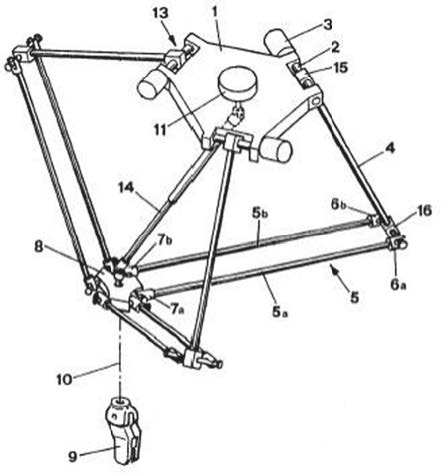
\includegraphics[height=0.25\textwidth,keepaspectratio]{assets/img/delta结构简图.jpg}
  \caption{Delta 并联机器人结构简图}
  \label{fig:delta-structure}
\end{figure}


\subsection{应用领域}
本作品可应用于曲面喷涂、工业点胶、柔性共形电子制造及教学科研验证等场景。
在工业表面处理中，系统可保持末端与工件表面的稳定距离，降低曲率变化导致的涂层厚度不均；
在电子制造中，可用于非平面基底上的导电油墨、锡膏或功能材料路径沉积，探索突破传统 PCB 平面布线限制的制造方式。直接书写与嵌入式 3D 打印等研究表明，功能材料沉积可用于柔性传感与软电子结构制备\cite{lewis2006diw,muth2014embedded,valentine2017soft}。
面向航空航天与智能装备，该平台可服务于机翼蒙皮、雷达罩、壳体外表面等复杂曲面上的传感器、天线和互连线路制备；
面向新型机器人产业，该平台可用于制作电子皮肤（即柔性传感器），作为机器人的重要感官之一，是机器人感受真实物理世界的必要途径。

\begin{figure}[htbp]
  \centering
  \begin{minipage}[t]{0.46\textwidth}
    \centering
    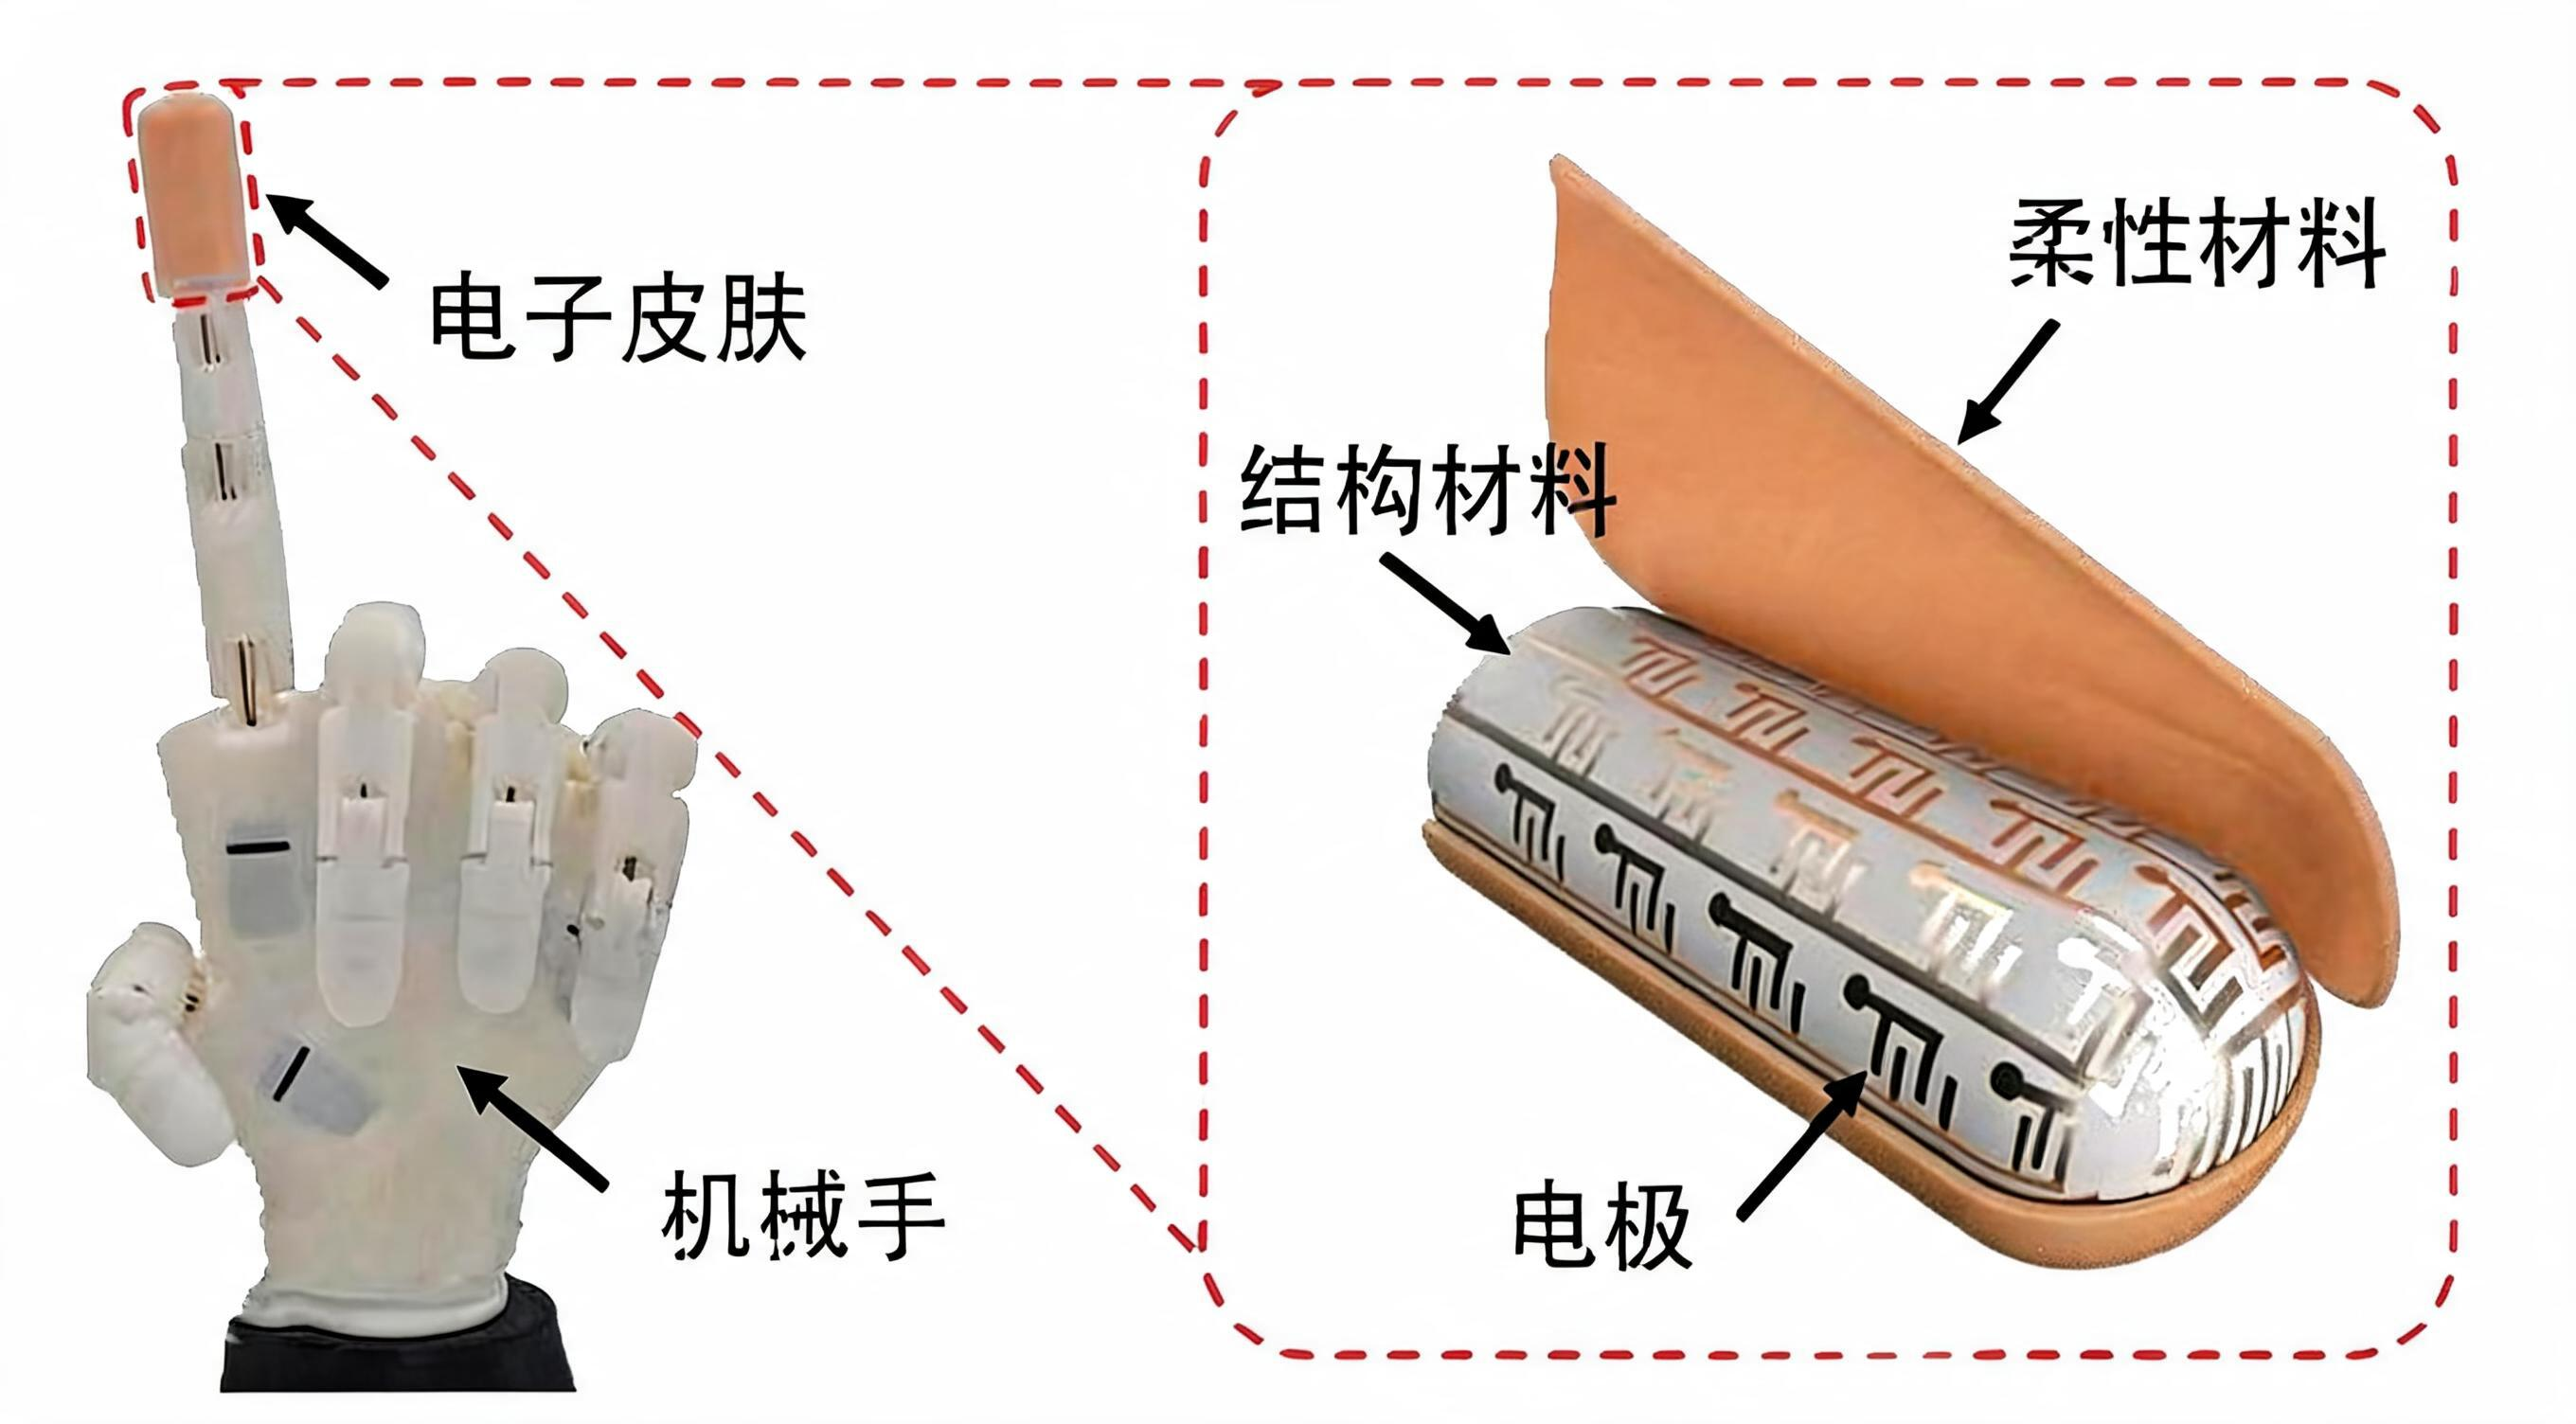
\includegraphics[width=\linewidth,height=0.22\textheight,keepaspectratio]{assets/img/电子皮肤.jpeg}\\[0.2em]
    {\small （a）机器人电子皮肤}
  \end{minipage}
  \hfill
  \begin{minipage}[t]{0.46\textwidth}
    \centering
    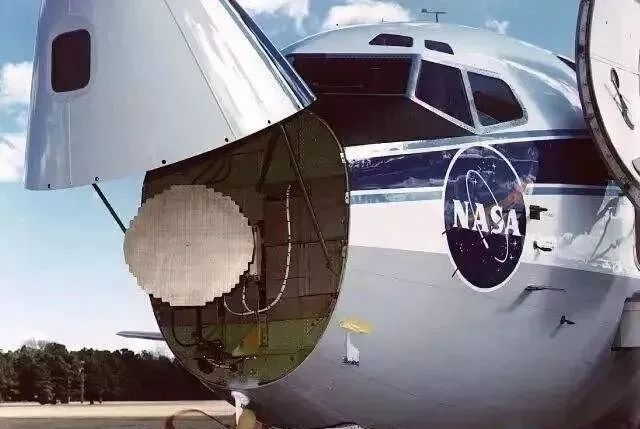
\includegraphics[width=\linewidth,height=0.22\textheight,keepaspectratio]{assets/img/飞机雷达罩.jpeg}\\[0.2em]
    {\small （b）航空雷达罩曲面载体}
  \end{minipage}
  \caption{应用场景资料图}
\end{figure}

\subsection{主要技术特点}
作品总体技术路线为“上位机规划 + 下位机控制 + Delta 并联执行”。
\begin{itemize}
  \item 下位机以 STM32F407 为核心控制器，利用其浮点运算能力完成运动控制、通信解析和任务调度。
  \item 机械部分采用 Delta 并联机构，通过运动学建模与逆解计算，将末端空间位姿转换为三轴电机运动指令\cite{hadfield2020delta}。
  \item 驱动部分采用闭环步进电机，实现多轴同步控制，提升运动响应速度和执行稳定性。
  \item 感知部分结合单目视觉完成工件定位、曲面配准与高度估计，为后续轨迹补偿提供空间基准\cite{zhang2000calibration,garrido2014aruco,olson2011apriltag}。
  \item 轨迹规划部分将平面图案或路径转换为带 Z 向补偿的曲面恒距轨迹，保证末端与工件表面保持稳定距离。
  \item 上位机与下位机通过无线方式通信，可完成参数下发、轨迹传输、运行控制和状态反馈。
\end{itemize}


\subsection{主要性能指标}
\begin{table}[h]
  \centering
  \begin{tabular}{p{0.32\textwidth}p{0.52\textwidth}}
    \toprule
    指标 & 数值或说明 \\
    \midrule
    有效工作范围 & X/Y $\approx \pm 120$\,mm，Z $\approx$ 210\,mm \\
    整机尺寸 & $\sim$300 $\times$ 300 $\times$ 500\,mm（长$\times$宽$\times$高） \\
    重复定位精度 & $\pm 0.05 \sim 0.1$\,mm（200脉冲/转 + 16细分） \\
    视觉标定前误差 & RMS XY = 3.10\,mm，最大 4.82\,mm \\
    视觉标定后误差 & RMS XY = 0.41\,mm，最大 1.04\,mm \\
    最高运动速度/加速度 & v=500$\sim$800\,mm/s，a=2000$\sim$5000\,mm/s$^2$ \\
    通信距离 & 局域网无线通信，室内稳定距离 30$\sim$50\,m \\
    \bottomrule
  \end{tabular}
  \caption{主要性能指标}
\end{table}

\subsection{主要创新点}
\begin{itemize}
  \item 为工业中常用于高速分拣的 Delta 并联机构引入曲面恒距作业的能力，发挥其 Z 向响应快、末端惯量小的优势\cite{clavel1988delta}，从而拓展更多应用场景。
  \item 融合单目视觉配准与运动学补偿，实现非规则曲面上的自适应高度修正和轨迹生成。
  \item 采用可更换末端与远程挤出设计，降低末端负载并提升速度上限，使平台兼顾喷印、点胶、书写、激光等多种作业模式。
  \item 集成上位机、控制器和执行机构，形成从图案/模型输入到曲面作业执行的完整流程，并支持联网与脱机两种运行方式，从而实现更灵活的作业形式。
\end{itemize}


\subsection{设计流程}
本设计流程如图~\ref{fig:design-flow} 所示。
经需求分析与多方选型对比，确定 Delta 机构、STM32 控制器和单目视觉的总体方案，
再依次完成机构与控制算法设计、上位机开发、系统联调及测试优化，
最终形成可持续迭代的平台化设计。

\begin{figure}[htbp]
\centering
\resizebox{\textwidth}{!}{%
\begin{tikzpicture}[
  node distance=2mm and 3mm,
  box/.style={draw, rounded corners, align=center, minimum width=16mm, minimum height=6.5mm, font=\small, fill=#1},
  box/.default={blue!8},
  arrow/.style={-Stealth, draw, thick},
  decision/.style={diamond, draw, align=center, aspect=1.5, font=\footnotesize, fill=yellow!12, inner sep=1pt},
]
\node[decision] (cmp_ctrl) {STM32 vs\\树莓派/ESP32};
\node[box=blue!15, left=of cmp_ctrl] (req) {需求分析};
\node[decision, above=of cmp_ctrl] (cmp_mech) {Delta vs\\SCARA/六轴};
\node[decision, below=of cmp_ctrl] (cmp_vis) {单目\\vs VL53L0X};

\node[box=green!15, right=of cmp_mech] (mech) {Delta\\并联};
\node[box=green!15, right=of cmp_ctrl] (ctrl) {STM32\\控制器};
\node[box=green!15, right=of cmp_vis] (vis) {单目\\视觉};

\node[box, right=of ctrl] (design) {机械建模+运动学\\+多轴控制算法};
\node[box, right=of design] (app) {上位机\\开发};
\node[box, right=of app] (integrate) {装配+标定\\+轨迹+联调};
\node[box=purple!10, right=of integrate] (test) {喷印测试\\+误差优化\\+末端拓展};

\draw[arrow] (req.east) -- ++(1.5mm,0) |- (cmp_mech.west);
\draw[arrow] (req.east) -- ++(1.5mm,0) |- (cmp_ctrl.west);
\draw[arrow] (req.east) -- ++(1.5mm,0) |- (cmp_vis.west);

\draw[arrow] (cmp_mech) -- (mech);
\draw[arrow] (cmp_ctrl) -- (ctrl);
\draw[arrow] (cmp_vis) -- (vis);

\draw[arrow] (mech.east) -| (design.north);
\draw[arrow] (ctrl.east) -- (design.west);
\draw[arrow] (vis.east) -| (design.south);

\draw[arrow] (design) -- (app);
\draw[arrow] (app) -- (integrate);
\draw[arrow] (integrate) -- (test);

\draw[arrow, rounded corners, gray] (test.south) -- ++(0,-2mm) -| (design.south);
\draw[arrow, rounded corners, gray] (test.north) -- ++(0,2mm) -| ([yshift=1mm]req.north);
\path ([yshift=2mm]req.north) -- ([yshift=2mm]test.north) node[above, midway, font=\small\itshape, gray!70] {可持续迭代};
\end{tikzpicture}%
}
\caption{设计流程}
\label{fig:design-flow}
\end{figure}

\partheading{第二部分}{系统组成及功能说明}


\subsection{整体介绍}
系统由上位机软件、视觉感知模块、嵌入式控制系统、Delta 并联执行机构和可更换末端执行器组成，整体采用“感知—规划—控制—执行”的工作流程：
\begin{itemize}
  \item \textbf{上位机}：负责模型导入、参数配置、轨迹预览、曲面补偿路径规划和 G-code 生成；
  \item \textbf{视觉模块}：负责采集工件图像，完成工件定位、曲面配准和高度信息获取，为轨迹补偿提供空间基准；
  \item \textbf{STM32F407 控制器}：作为下位机核心，接收上位机下发的轨迹与控制参数，完成通信解析、运动学计算和多轴运动指令分发；
  \item \textbf{闭环步进电机及驱动器}：带动 Delta 并联机构运动，使末端按照规划轨迹在工作空间内高速、稳定地移动；
  \item \textbf{末端执行器}：可根据任务切换为书写、激光、点胶或喷印模块，实现平面书写、曲面恒距喷印、点胶等不同作业。
\end{itemize}
\begin{figure}[htbp]
  \centering
  \resizebox{\textwidth}{!}{%
    \begin{tikzpicture}[
      font=\footnotesize,
      >=Stealth,
      stage/.style={draw,rounded corners=2mm,text width=2.25cm,minimum height=0.78cm,align=center,inner sep=2.5pt,fill=gray!10},
      soft/.style={stage,fill=blue!8,draw=blue!55},
      hard/.style={stage,fill=orange!10,draw=orange!70!black},
      comm/.style={stage,text width=2.05cm,minimum height=0.68cm,fill=green!8,draw=green!45!black,font=\scriptsize},
      arrow/.style={->,thick},
      dashedarrow/.style={->,thick,dashed},
      layer/.style={draw,rounded corners=2mm,dashed,inner sep=7pt}
    ]
      \node[soft] (s1) at (0,2.15) {视觉处理\\标定/配准\\高度估计};
      \node[soft] (s2) at (3.15,2.15) {Flutter 上位机\\模型导入\\轨迹规划};
      \node[soft] (s3) at (6.30,2.15) {Moonraker\\G-code解析/状态监控};
      \node[soft] (s4) at (9.45,2.15) {任务执行管理\\文件上传\\启动运行};

      \node[comm] (c1) at (0,0.62) {图像快照\\HTTP/本地相机服务};
      \node[comm,text width=2.35cm] (c2) at (3.15,0.62) {局域网通信\\Moonraker HTTP\\+ WebSocket};
      \node[comm] (c3) at (6.3,0.62) {控制链路\\USB 串口\\MCU};

      \node[hard] (h1) at (0,-0.95) {单目摄像头\\工件/曲面图像};
      \node[hard] (h2) at (3.15,-0.95) {工作台与工件\\坐标基准};
      \node[hard] (h3) at (6.30,-0.95) {STM32F407\\运动解算\\脉冲输出};
      \node[hard] (h4) at (9.45,-0.95) {闭环驱动+Delta机构\\末端执行器作业};
      \node[comm] (c4) at (7.88,-2.20) {驱动信号\\STEP/DIR/EN\\或 UART};

      \draw[arrow] (h1.north) -- (c1.south);
      \draw[arrow] (c1.north) -- (s1.south);
      \draw[arrow] (s1.east) -- node[above,font=\scriptsize]{图像} node[below,font=\scriptsize]{参数}(s2.west);
      \draw[arrow] (s2.east) -- (s3.west);
      \draw[arrow] (s3.east) -- node[above,font=\scriptsize]{状态}node[below,font=\scriptsize]{反馈} (s4.west);

      \draw[arrow] (s2.south) -- (c2.north);
      \draw[arrow] (c2.east) -- (c3.west);
      \draw[arrow] (s3.south) -- (c3.north);
      \draw[arrow] (c3.south) -- (h3.north);

      \draw[arrow] (h2.east) -- node[above,font=\scriptsize]{作业} node[below,font=\scriptsize]{基准} (h3.west);
      \draw[arrow] (h3.east) -- (h4.west);
      \draw[arrow] (h3.south) |- (c4.west);
      \draw[arrow] (c4.east) -| (h4.south);

      \draw[dashedarrow] (h4.east) -- ++(0.6,0) coordinate (fb) |- (s4.east);
      \node[font=\scriptsize,anchor=east] at (fb |- 0,0.72) {运行状态};
      \node[font=\scriptsize,anchor=west] at (fb |- 0,0.72) {误差验证};

      \begin{scope}[on background layer]
        \node[layer,fit=(s1)(s2)(s3)(s4)] {};
        \node[layer,fit=(h1)(h2)(h3)(h4)(c4)] {};
      \end{scope}

      \node[font=\bfseries] at (-2.2,2.15) {软件层};
      \node[font=\bfseries] at (-2.2,0.72) {通信层};
      \node[font=\bfseries] at (-2.2,-0.95) {硬件层};
      \node[font=\bfseries] at (0,3.8) {感知};
      \node[font=\bfseries] at (3.15,3.8) {规划};
      \node[font=\bfseries] at (6.30,3.8) {控制};
      \node[font=\bfseries] at (9.45,3.8) {执行};
      \draw[arrow] (-0.65,3.4) -- (10.20,3.4);
    \end{tikzpicture}%
  }
  \caption{系统总体框架与软硬件通信关系}
\end{figure}

\subsection{硬件系统介绍}

\subsubsection{硬件整体介绍}
本作品的硬件系统主要由 Delta 并联机械结构、三组闭环步进电机及驱动器、STM32F407 主控板、单目摄像头模块、可更换末端执行器、无线通信模块、电源模块以及机架和工作台组成。

各硬件模块围绕"稳定支撑、精确运动、视觉感知、任务执行"四个目标进行设计：
\begin{itemize}
  \item \textbf{机架和工作台}：提供整体安装基准与作业空间；
  \item \textbf{Delta 并联机械结构}：作为核心运动机构，承担末端三维空间定位任务；
  \item \textbf{闭环步进电机及驱动器}：三组电机分别驱动三条运动支链，通过驱动器接收控制信号，实现同步运动；
  \item \textbf{STM32F407 主控板}：接收上位机指令、完成运动解算和电机控制信号输出；
  \item \textbf{单目摄像头模块}：采集工件和工作区图像，提供定位、配准和高度估计信息；
  \item \textbf{末端执行器}：位于动平台上，可更换为书写、激光、点胶或喷印等模块；
  \item \textbf{无线通信与显示屏幕}：用于上位机与控制端之间的数据传输，以及下位机运动状态的显示，并提供人机交互界面；
  \item \textbf{电源模块}：为主控、电机驱动、传感器和末端执行器提供稳定供电。
\end{itemize}

系统硬件各模块间按"感知—控制—驱动—执行"分层协作，数据流与反馈回路如图~\ref{fig:hw-flow}所示。

\begin{figure}[htbp]
\centering
\resizebox{\textwidth}{!}{%
\begin{tikzpicture}[
  box/.style={draw, rounded corners, align=center, minimum width=24mm, minimum height=8mm, font=\small, fill=#1},
  arrow/.style={-Stealth, draw, thick},
  fb/.style={-Stealth, draw, thick, dashed},
  layer/.style={draw, rounded corners=2mm, densely dotted, inner sep=6pt, fill=#1, fill opacity=0.08, text opacity=1},
]
\def\ctrlsep{13mm}      % 控制层上下节点间距
\def\routegap{7mm}      % 反馈线绕行间距
\def\layerpad{7pt}      % 虚线框内边距

\node[box=blue!12] (vis) at (0,0) {视觉模块\\工件定位/曲面配准};

\node[box=cyan!15] (pc) at (39mm,0) {上位机\\轨迹规划/参数};
\node[box=orange!15] (stm) at (39mm,-\ctrlsep) {STM32F407\\三轴指令输出};

\node[box=green!15] (drv) at (78mm,-\ctrlsep) {驱动器\\三轴控制};
\node[box=green!15] (mot) at (110mm,-\ctrlsep) {闭环步进\\编码器反馈};

\node[box=purple!12] (delta) at (145mm,-\ctrlsep) {Delta 机构\\转角→位移};
\node[box=purple!12] (ee) at (179mm,-\ctrlsep) {末端执行器\\喷印/点胶/书写};

\draw[arrow] (vis.east) -- (pc.west);
\draw[arrow] (pc.south) -- (stm.north);
\draw[arrow] (stm.east) -- (drv.west);
\draw[arrow] (drv.east) -- (mot.west);
\draw[arrow] (mot.east) -- (delta.west);
\draw[arrow] (delta.east) -- (ee.west);

\draw[fb] (vis.south) -- ++(0,-\routegap) -- (stm.west);
\draw[fb] (mot.north) -- ++(0,\routegap) -| (drv.north);

\begin{scope}[on background layer]
  \node[layer=blue!20, fit=(vis), inner sep=\layerpad] (l_sense) {};
  \node[layer=orange!20, fit=(pc)(stm), inner sep=\layerpad] (l_ctrl) {};
  \node[layer=green!20, fit=(drv)(mot), inner sep=\layerpad] (l_drv) {};
  \node[layer=purple!20, fit=(delta)(ee), inner sep=\layerpad] (l_exec) {};
\end{scope}
\node[above=0.5mm of l_sense, font=\small\bfseries] {感知};
\node[above=0.5mm of l_ctrl, font=\small\bfseries] {控制};
\node[above=13mm of l_drv, font=\small\bfseries] {驱动};
\node[above=13mm of l_exec, font=\small\bfseries] {执行};
\end{tikzpicture}%
}
\caption{硬件系统协调关系}
\label{fig:hw-flow}
\end{figure}
\subsubsection{机械设计介绍}
机械设计分为三大部分：机架与工作台、Delta 并联机械结构和末端执行器。
\paragraph{（1）机架和工作台}
机架和工作台由上至下依次分为三个区域：

\textbf{控制器安装区}：用于安装 STM32 主控板、电源模块等，如图\ref{fig:frame-installation}所示。

\textbf{运动执行区}：安装 Delta 并联机械结构，详见“Delta 并联机械结构”部分。

\textbf{工作台支撑区}：提供工件放置平台，支撑整个作业区域，如图\ref{fig:workbench-support}所示。

\begin{figure}[htbp]
  \centering
  \begin{minipage}[t]{0.48\textwidth}
    \centering
    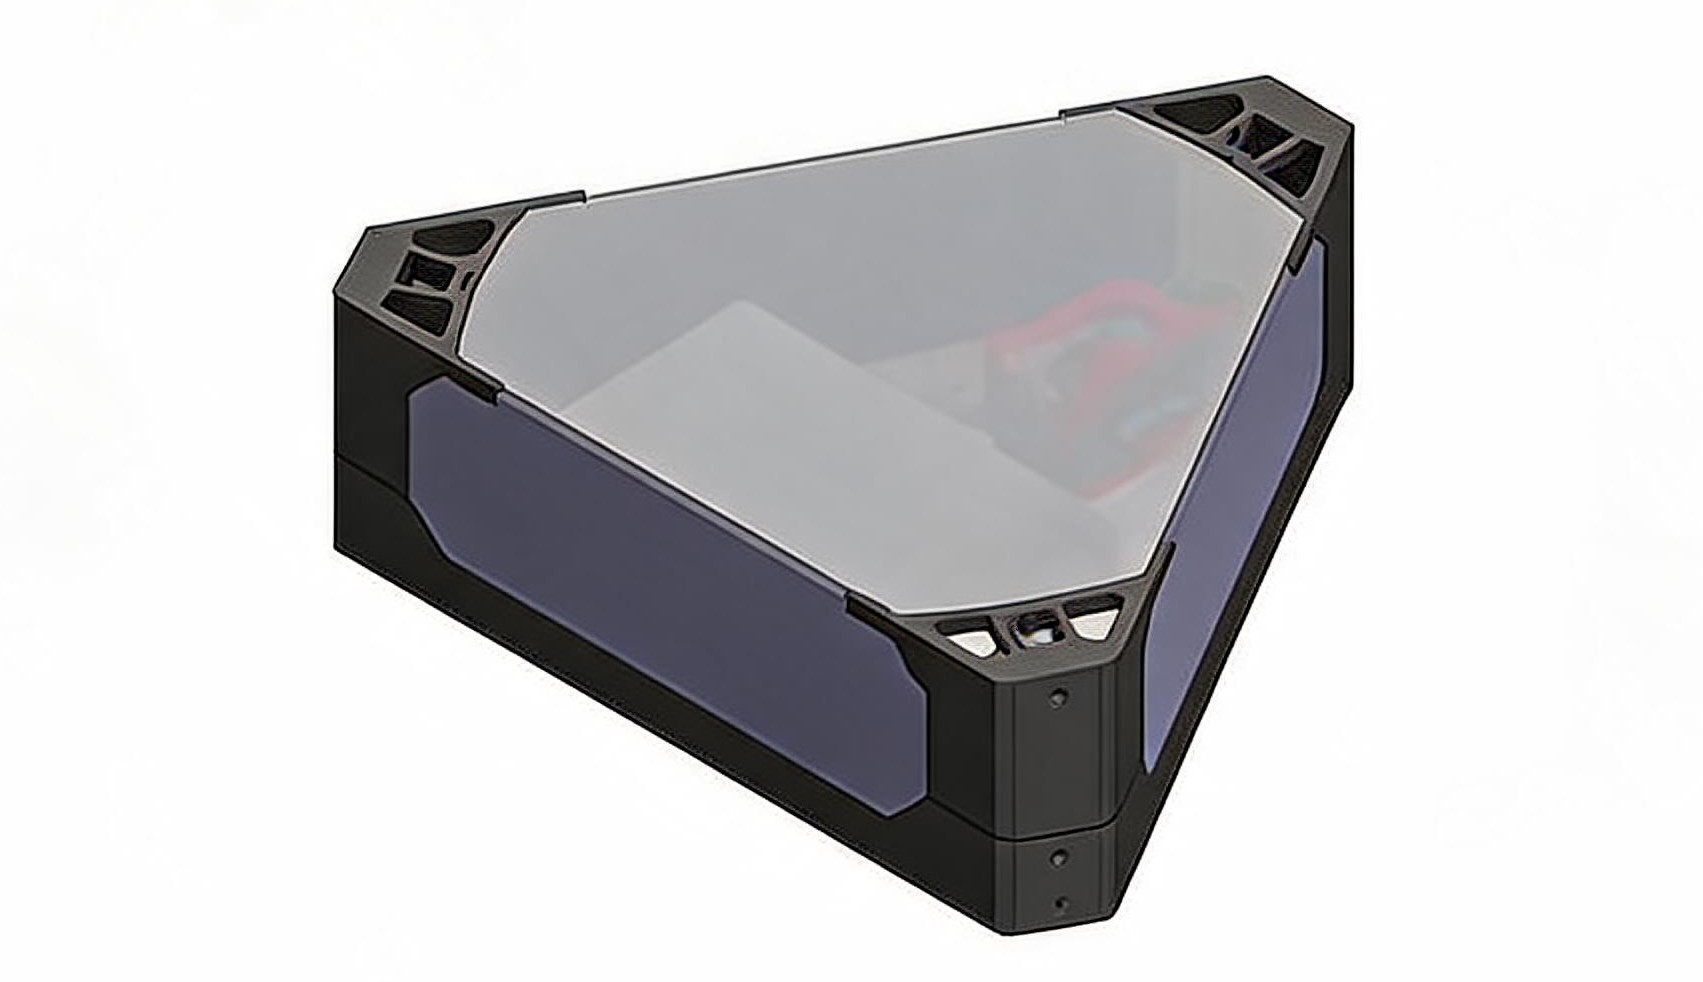
\includegraphics[width=\linewidth,keepaspectratio]{assets/img/控制器安装区.jpeg}
    \caption{控制器安装区示意图}
    \label{fig:frame-installation}
  \end{minipage}
  \hfill
  \begin{minipage}[t]{0.48\textwidth}
    \centering
    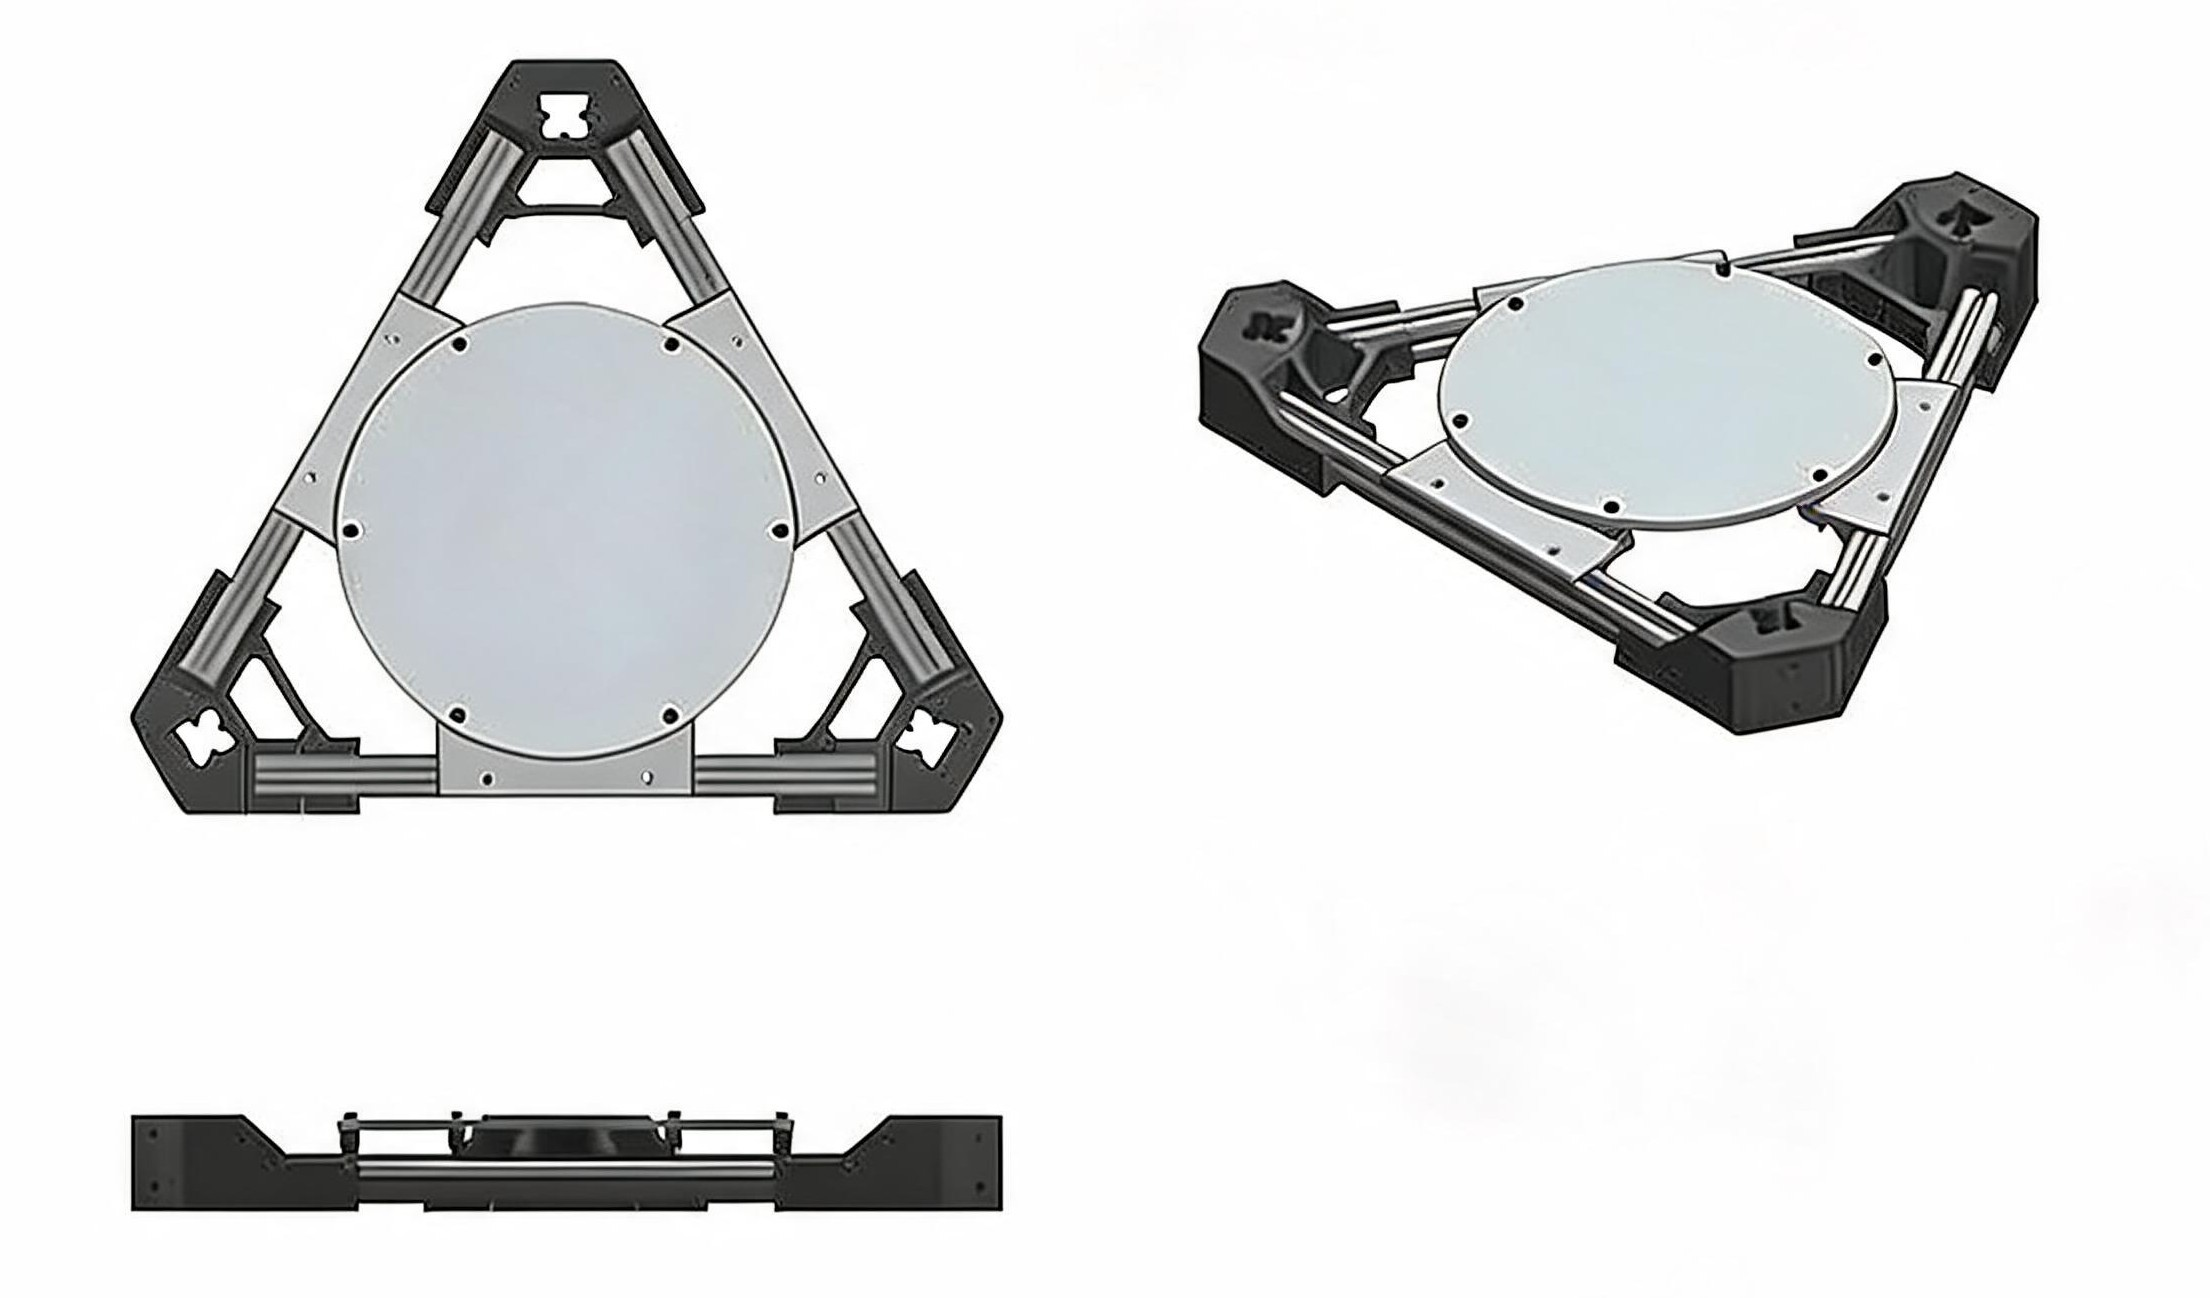
\includegraphics[width=\linewidth,keepaspectratio]{assets/img/工作台支撑区.jpeg}
    \caption{工作台支撑区示意图}
    \label{fig:workbench-support}
  \end{minipage}
\end{figure}

\paragraph{（2）Delta 并联机械结构}
Delta 并联机构由基座、三条运动支链及其协同驱动的末端动平台组成，整体结构如图\ref{fig:delta-structure-detail}所示：
\begin{figure}[htbp]
  \centering
  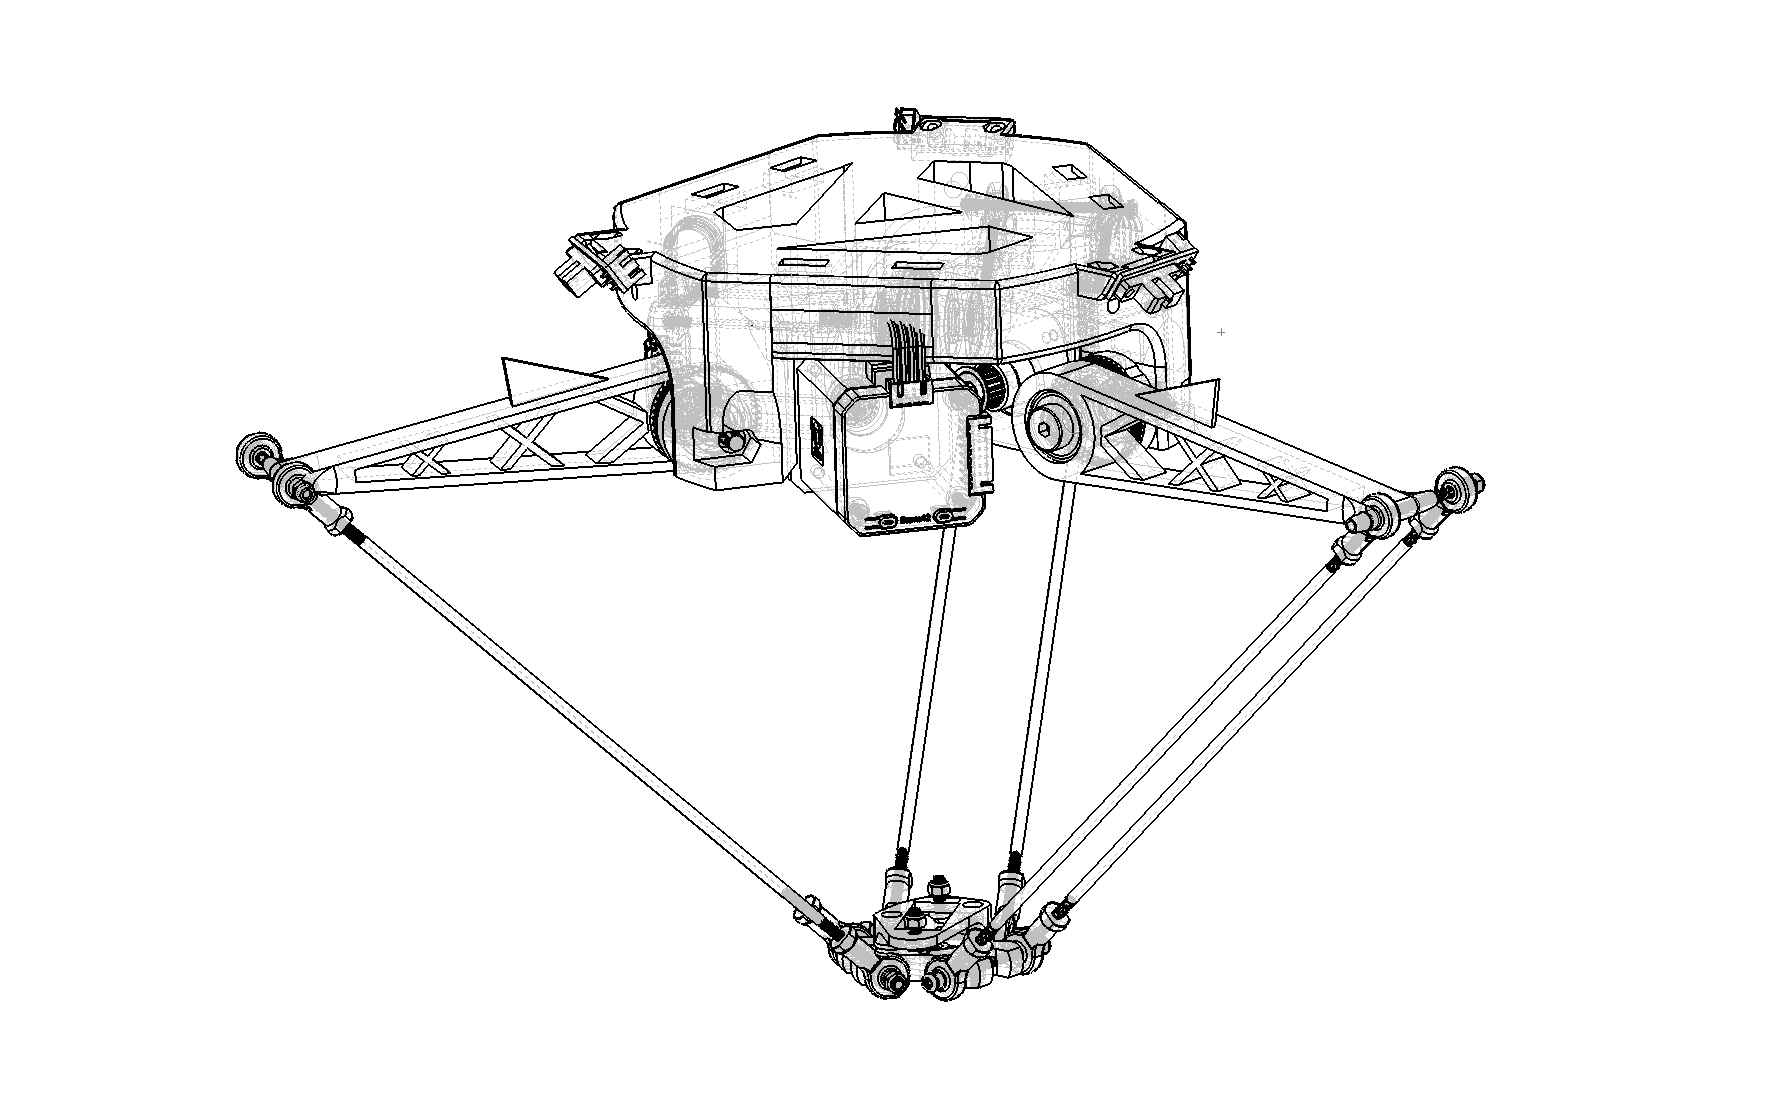
\includegraphics[width=0.6\textwidth,keepaspectratio]{assets/img/delta结构图.png}
  \caption{Delta 并联机构示意图}
  \label{fig:delta-structure-detail}
\end{figure}

\textbf{基座}：用于安装固定步进电机，并使三条上臂运动支点相对于结构中心保持 120\textdegree{} 间隔，
保证机构对称性和运动稳定性，并为后续运动解算提供便利。如图\ref{fig:base-structure}所示：
\begin{figure}[htbp]
  \centering
  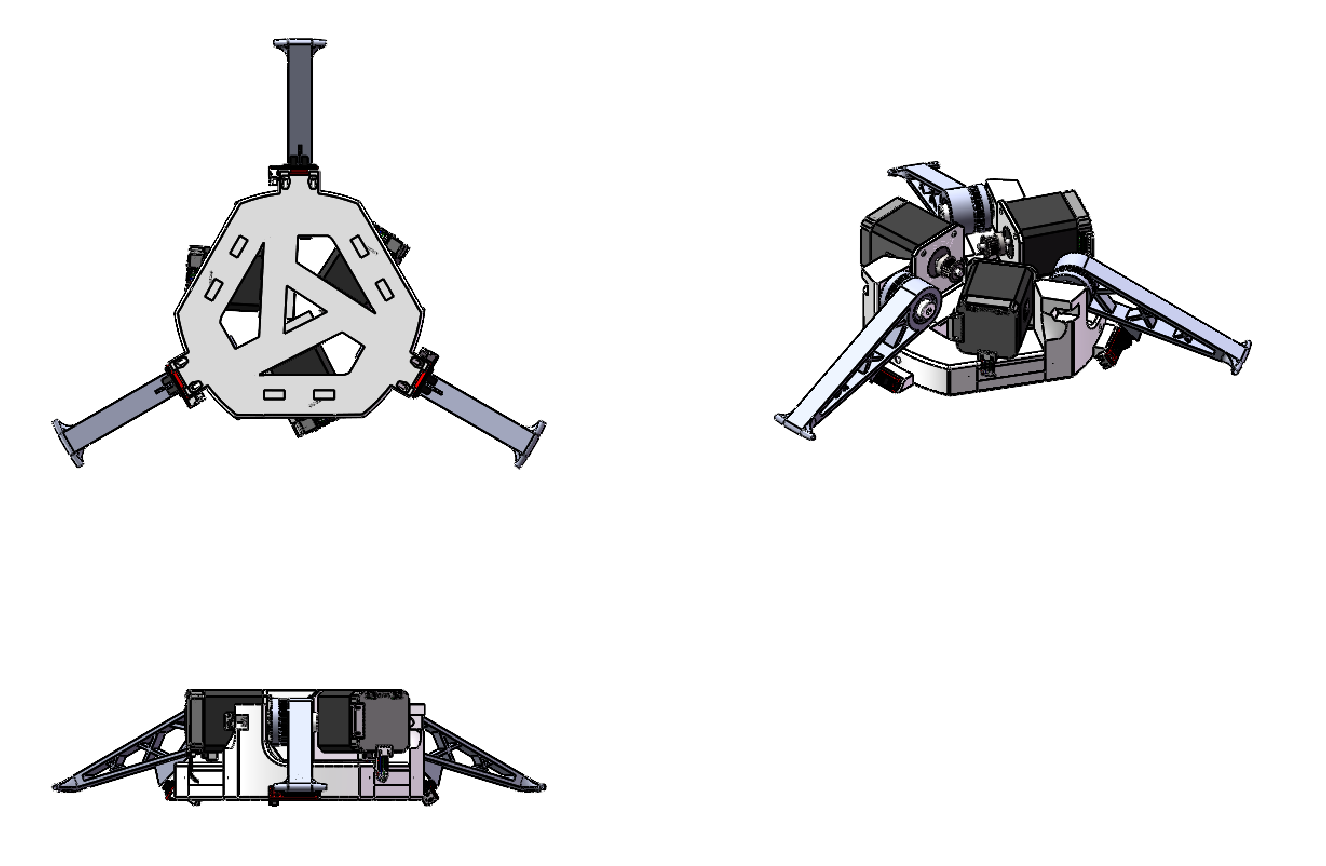
\includegraphics[width=0.8\textwidth,keepaspectratio]{assets/img/静平台.PNG}
  \caption{基座示意图}
  \label{fig:base-structure}
\end{figure}

此外，基座上还安装有单目摄像头模块，用于采集工件图像，完成工件定位、曲面配准和高度估计，为轨迹补偿提供空间基准。
摄像头的安装位置如图\ref{fig:camera-installation}所示：
\begin{figure}[htbp]
  \centering
  \begin{minipage}[t]{0.48\textwidth}
    \centering
    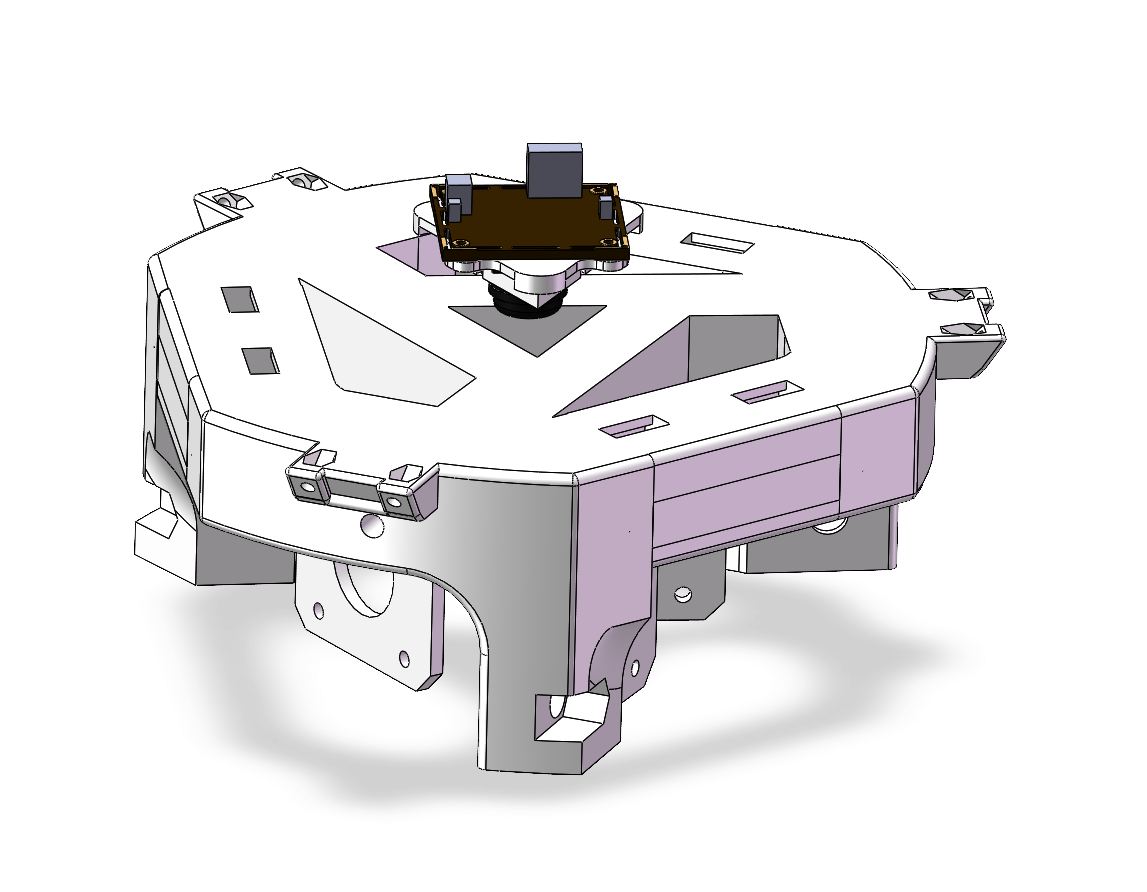
\includegraphics[width=\linewidth,keepaspectratio]{assets/img/摄像头安装.PNG}
    \caption{摄像头安装示意图}
    \label{fig:camera-installation}
  \end{minipage}
  \hfill
  \begin{minipage}[t]{0.48\textwidth}
    \centering
    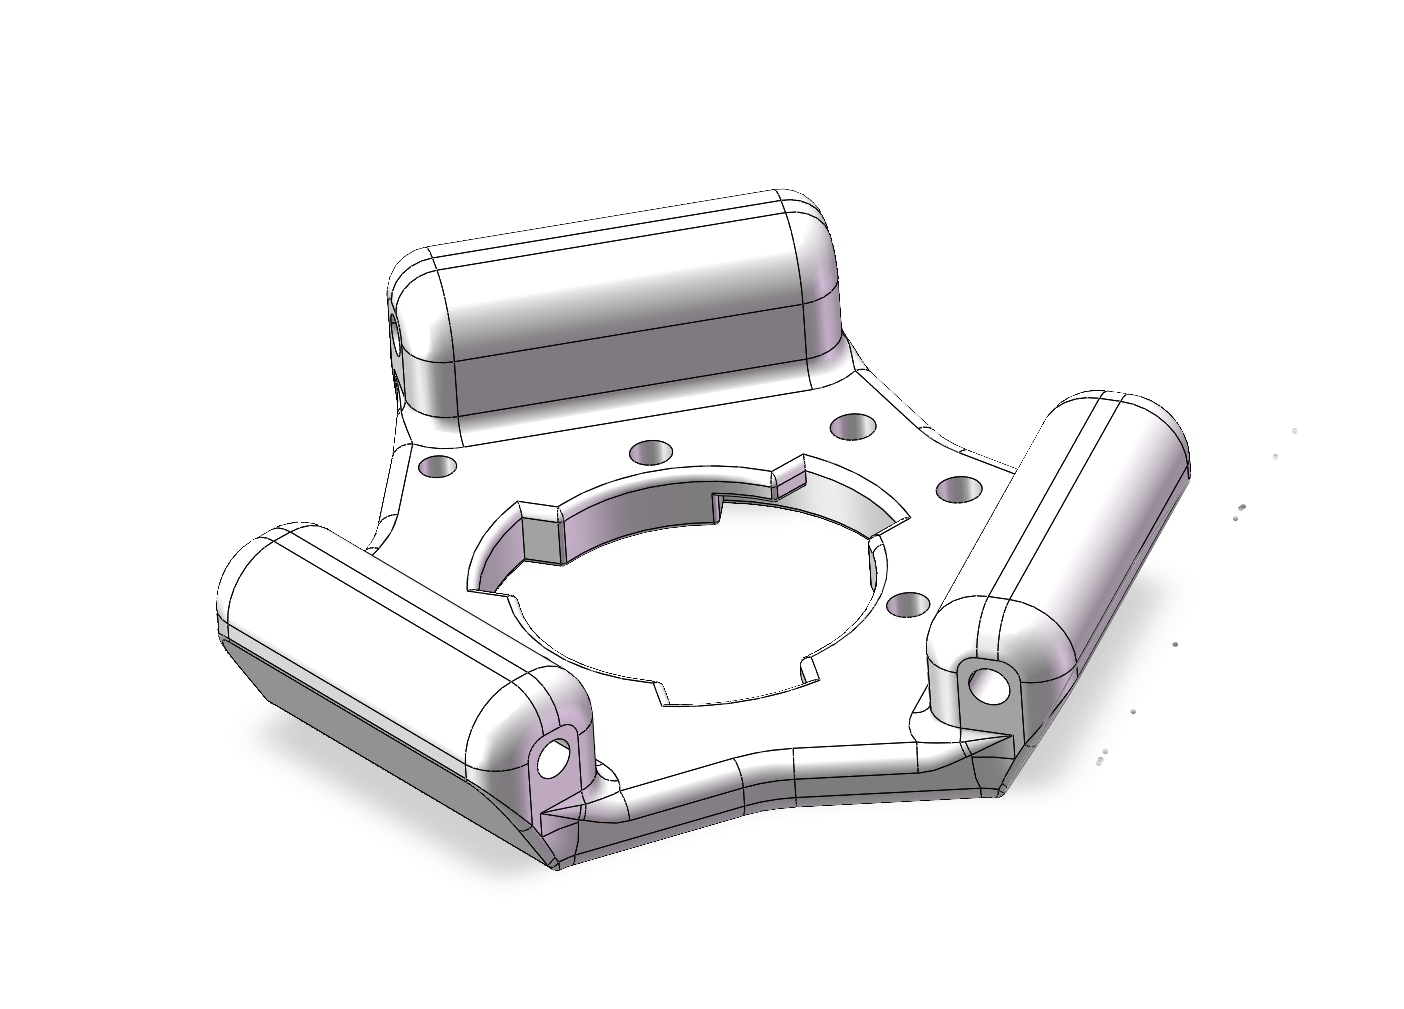
\includegraphics[width=\linewidth,keepaspectratio]{assets/img/动平台.PNG}
    \caption{末端动平台示意图}
    \label{fig:end-effector-platform}
  \end{minipage}
\end{figure}

\textbf{运动支链}：由三条相同的支链组成，
每条支链包括一个步进电机和相应的传动机构（传动比50:20，图\ref{fig:branch-structure}），一个上臂（类比人的大臂，图\ref{fig:upper-arm}），一个下臂（类比人的小臂,图\ref{fig:lower-arm}）
以及相应的上臂固定点（类比人的肩关节，图\ref{fig:branch-structure}）与上下臂之间的连接点（类比人的肘关节,图\ref{fig:joint}），用于驱动末端动平台进行空间运动。
\begin{figure}[htbp]
  \centering
  \begin{minipage}[t]{0.48\textwidth}
    \centering
    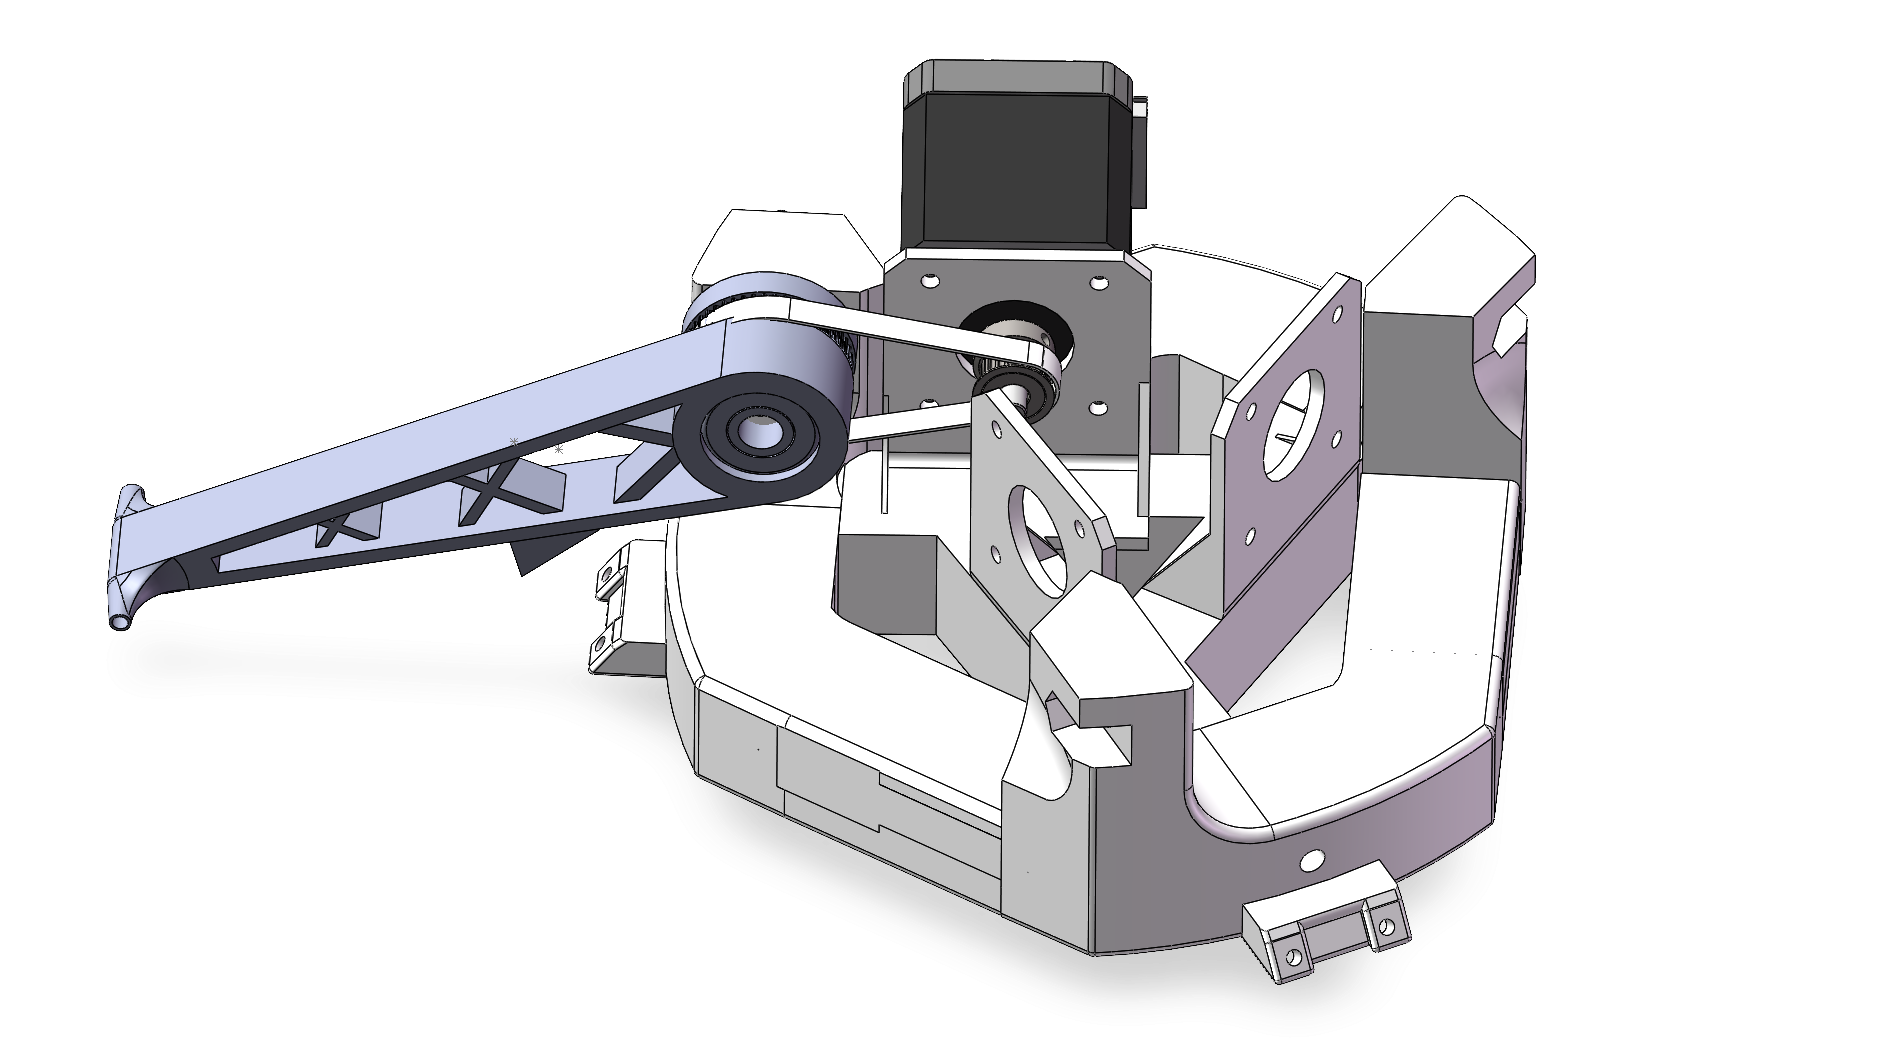
\includegraphics[width=\linewidth,keepaspectratio]{assets/img/传动机构.PNG}
    \caption{传动机构（肩关节）示意图}
    \label{fig:branch-structure}
  \end{minipage}
  \hfill
  \begin{minipage}[t]{0.4\textwidth}
    \centering
    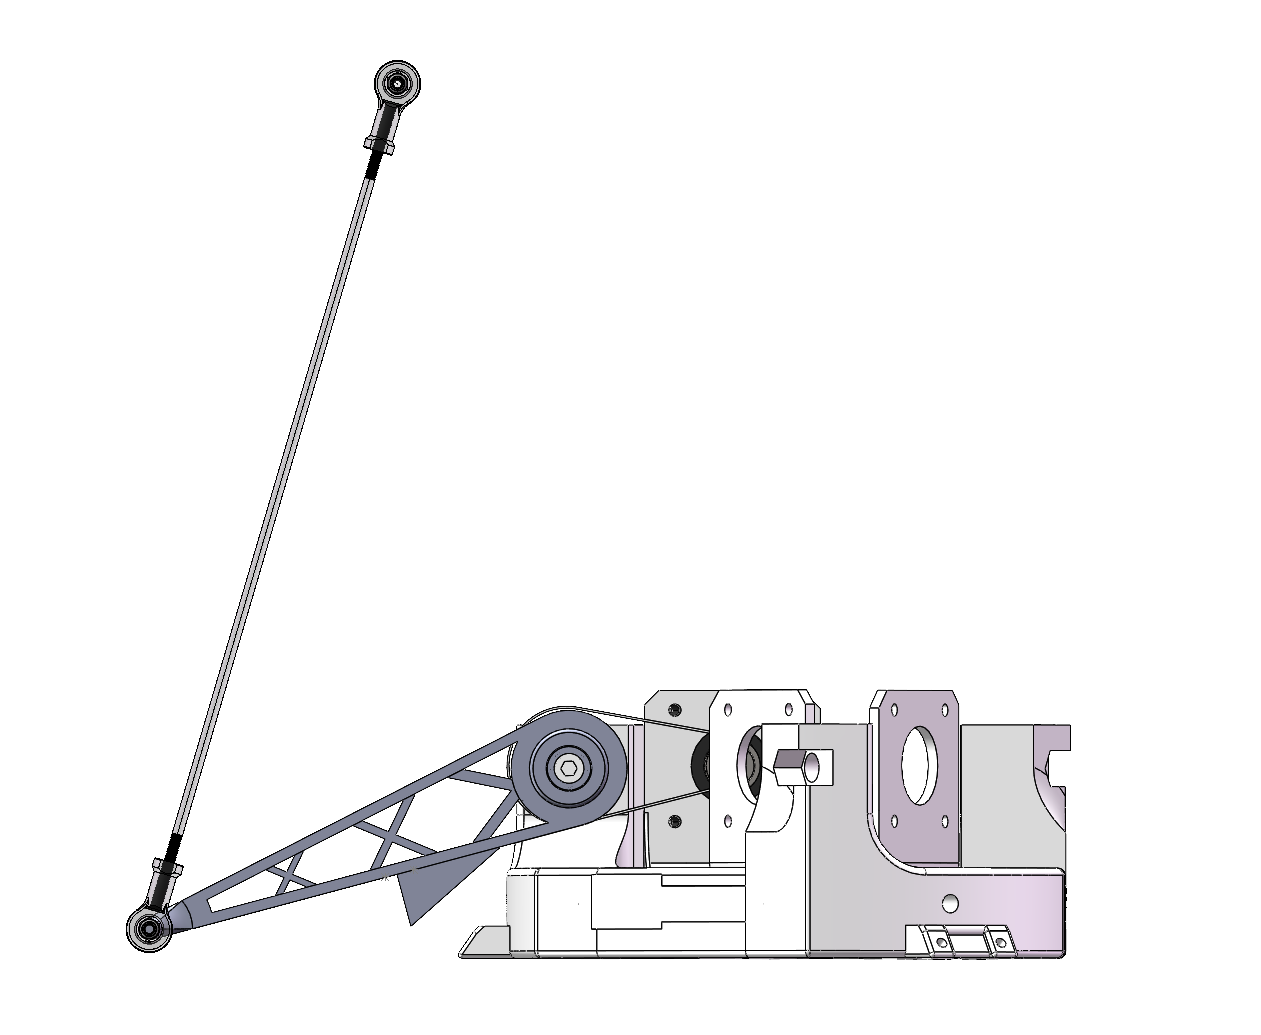
\includegraphics[width=\linewidth,keepaspectratio]{assets/img/运动支链.PNG}
    \caption{上下臂连接（肘关节）示意图}
    \label{fig:joint}
  \end{minipage}
\end{figure}
\begin{figure}[htbp]
  \centering
  \begin{minipage}[t]{0.48\textwidth}
    \centering
    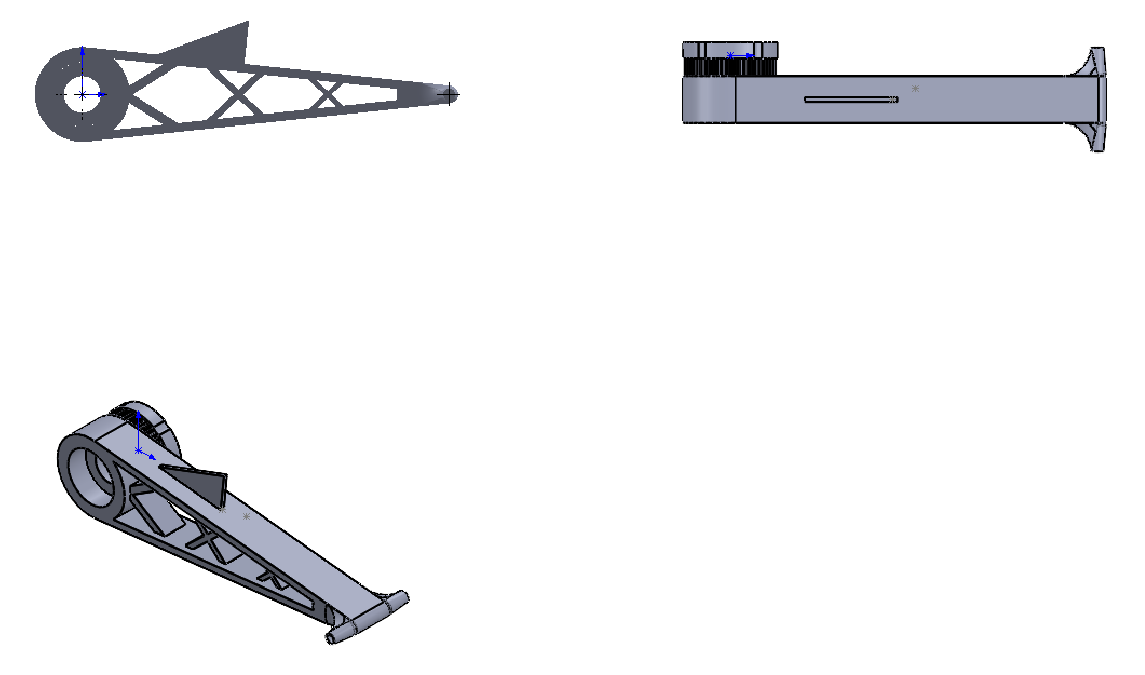
\includegraphics[width=\linewidth,keepaspectratio]{assets/img/大臂.PNG}
    \caption{上臂示意图}
    \label{fig:upper-arm}
  \end{minipage}
  \hfill
  \begin{minipage}[t]{0.48\textwidth}
    \centering
    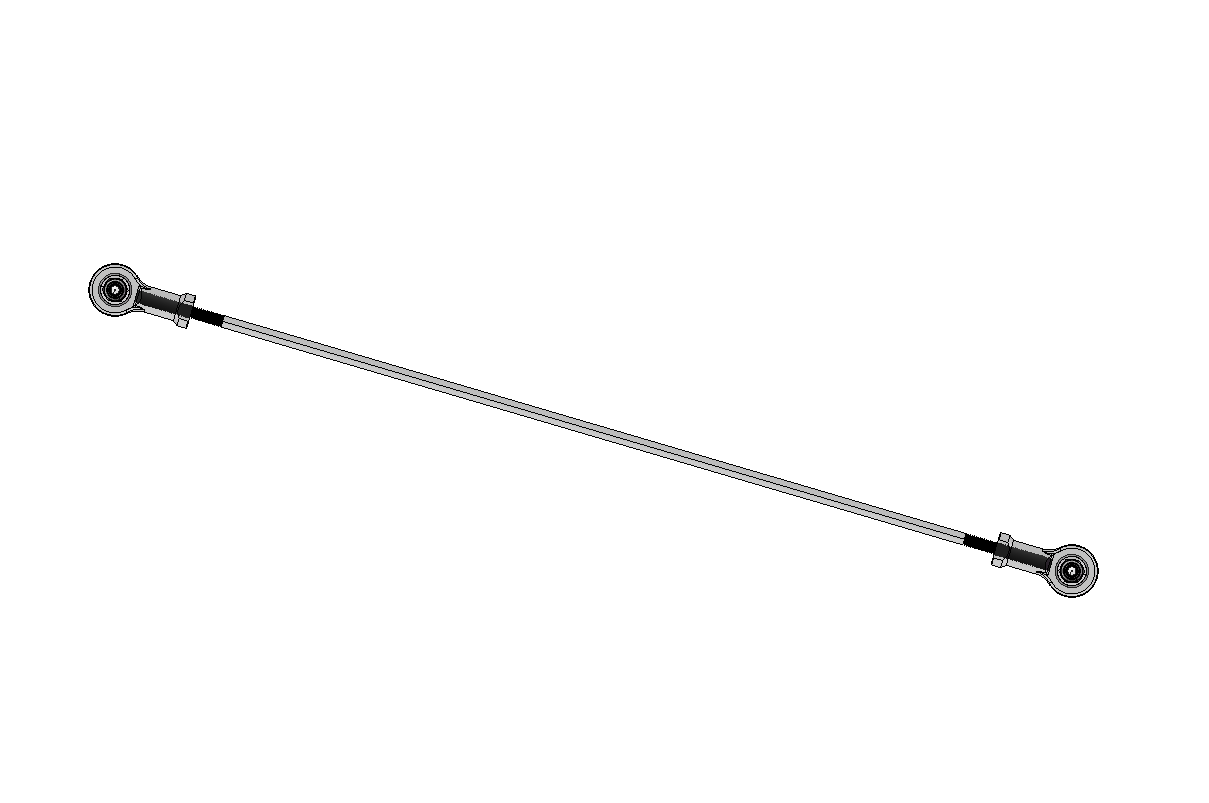
\includegraphics[width=\linewidth,keepaspectratio]{assets/img/小臂.PNG}
    \caption{下臂示意图}
    \label{fig:lower-arm}
  \end{minipage}
\end{figure}

\paragraph{（3）末端执行器}
针对不同作业场景，系统设计了多种末端执行器模块，包括挤出/点胶模块、激光模块、电磁铁模块和舵机云台模块等。
每个模块都可以通过旋转式卡槽与末端动平台快速连接和拆卸，便于在不同任务之间切换：

\textbf{挤出/点胶模块}：常见挤出/点胶驱动源包括蠕动泵、步进电机驱动丝杆、气压装置、压电微型泵等。
我们选择了步进电机驱动的丝杆作为挤出/点胶模块的核心驱动源，整体结构如图\ref{fig:pump}所示：
\begin{figure}[htbp]
  \centering
  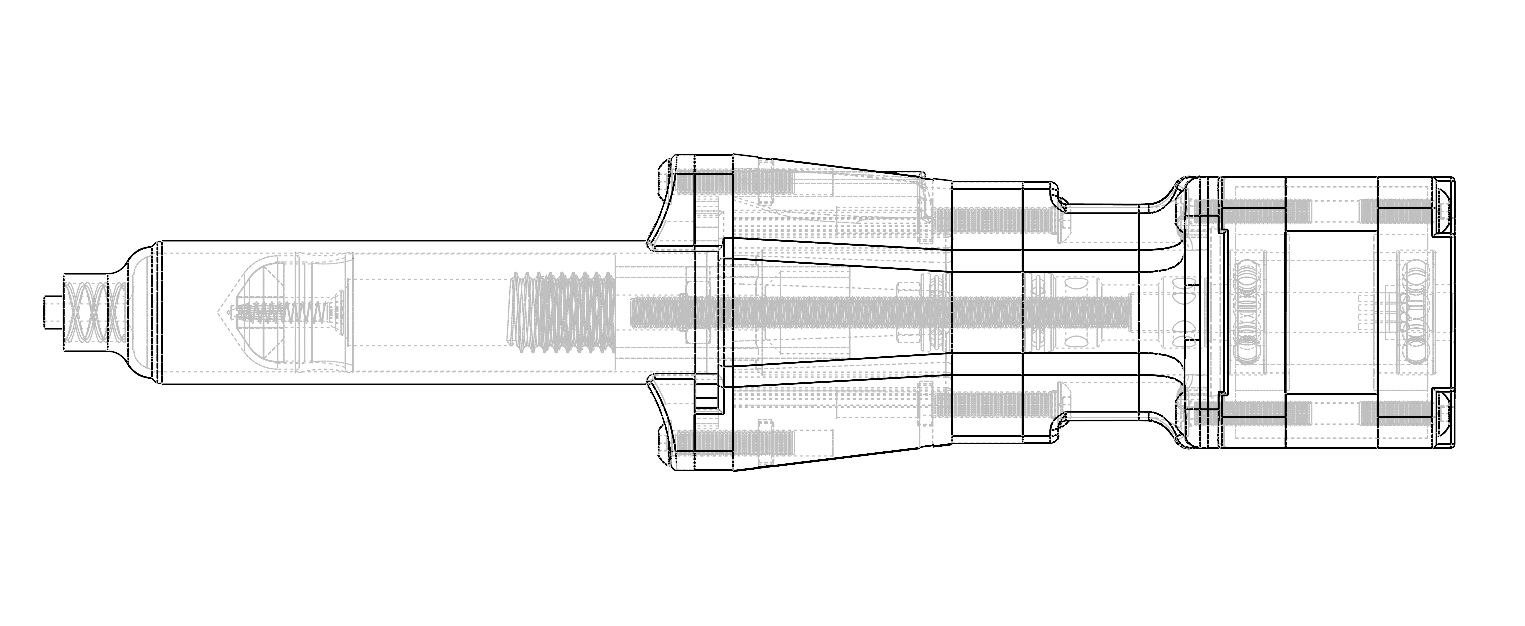
\includegraphics[width=0.8\textwidth,keepaspectratio]{assets/img/挤出装置 .PNG}
  \caption{挤出装置示意图}
  \label{fig:pump}
\end{figure}

该挤出机构的驱动原理可由其剖视图（图\ref{fig:pump-section}）来说明：
\begin{figure}[htbp]
  \centering
  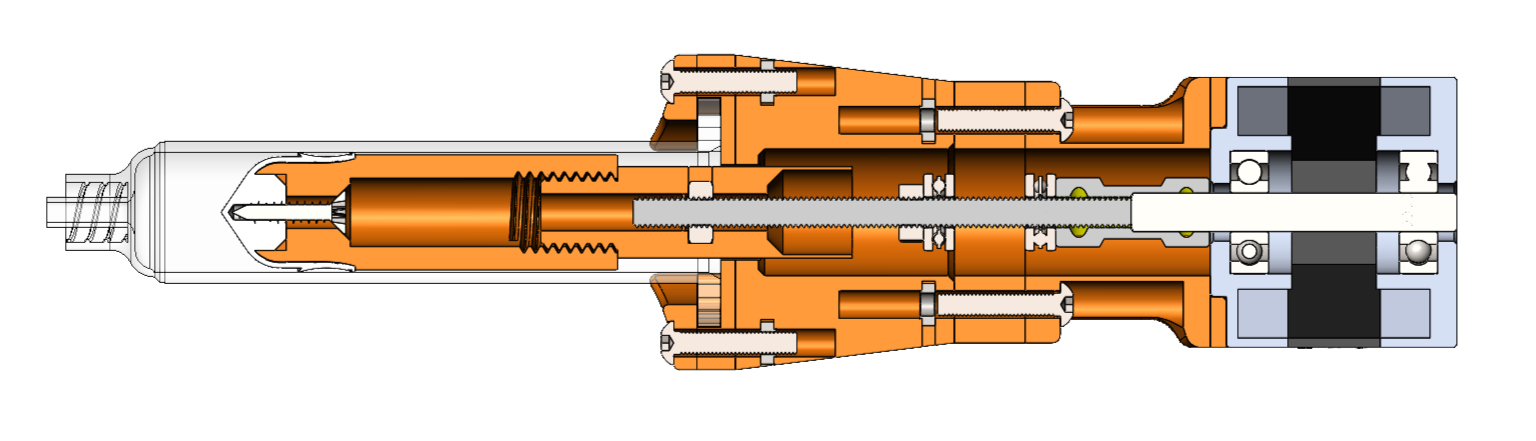
\includegraphics[width=0.8\textwidth,keepaspectratio]{assets/img/挤出装置剖视图.PNG}
  \caption{挤出装置剖视图}
  \label{fig:pump-section}
\end{figure}

通过联轴器将步进电机轴与丝杆连接，使丝杆与步进电机保持同步旋转。
丝杆与螺母配合后，将旋转运动转换为直线运动，并传递给挤出头，
从而实现针筒中的材料挤出。

为了减轻末端执行器的重量，我们将步进电机安装在机架上，通过带有鲁尔转接头的软管将丝杆与挤出头（如图\ref{fig:needle}所示）连接，
从而将挤出头的重量降至最小，提升 Delta 机构的运动响应速度和精度。

\textbf{电磁铁模块}：通过控制电磁铁的通断电实现对铁磁性工件的拾取与释放，
可用于物料分拣、棋子移动等场景，如图\ref{fig:electromagnet}所示。

\textbf{激光模块}：通过PWM控制激光头的功率输出，
可在纸张、木材等材料上进行激光雕刻和图样绘制，如图\ref{fig:lasers}所示。

\textbf{舵机云台模块}：通过两个自由度舵机驱动末端姿态调整，
可在喷印或点胶时保持工具与曲面法向对齐，扩展曲面作业的适应能力，如图\ref{fig:servo-gimbal}所示。

\begin{figure}[htbp]
  \centering
  \begin{minipage}[t]{0.48\textwidth}
    \centering
    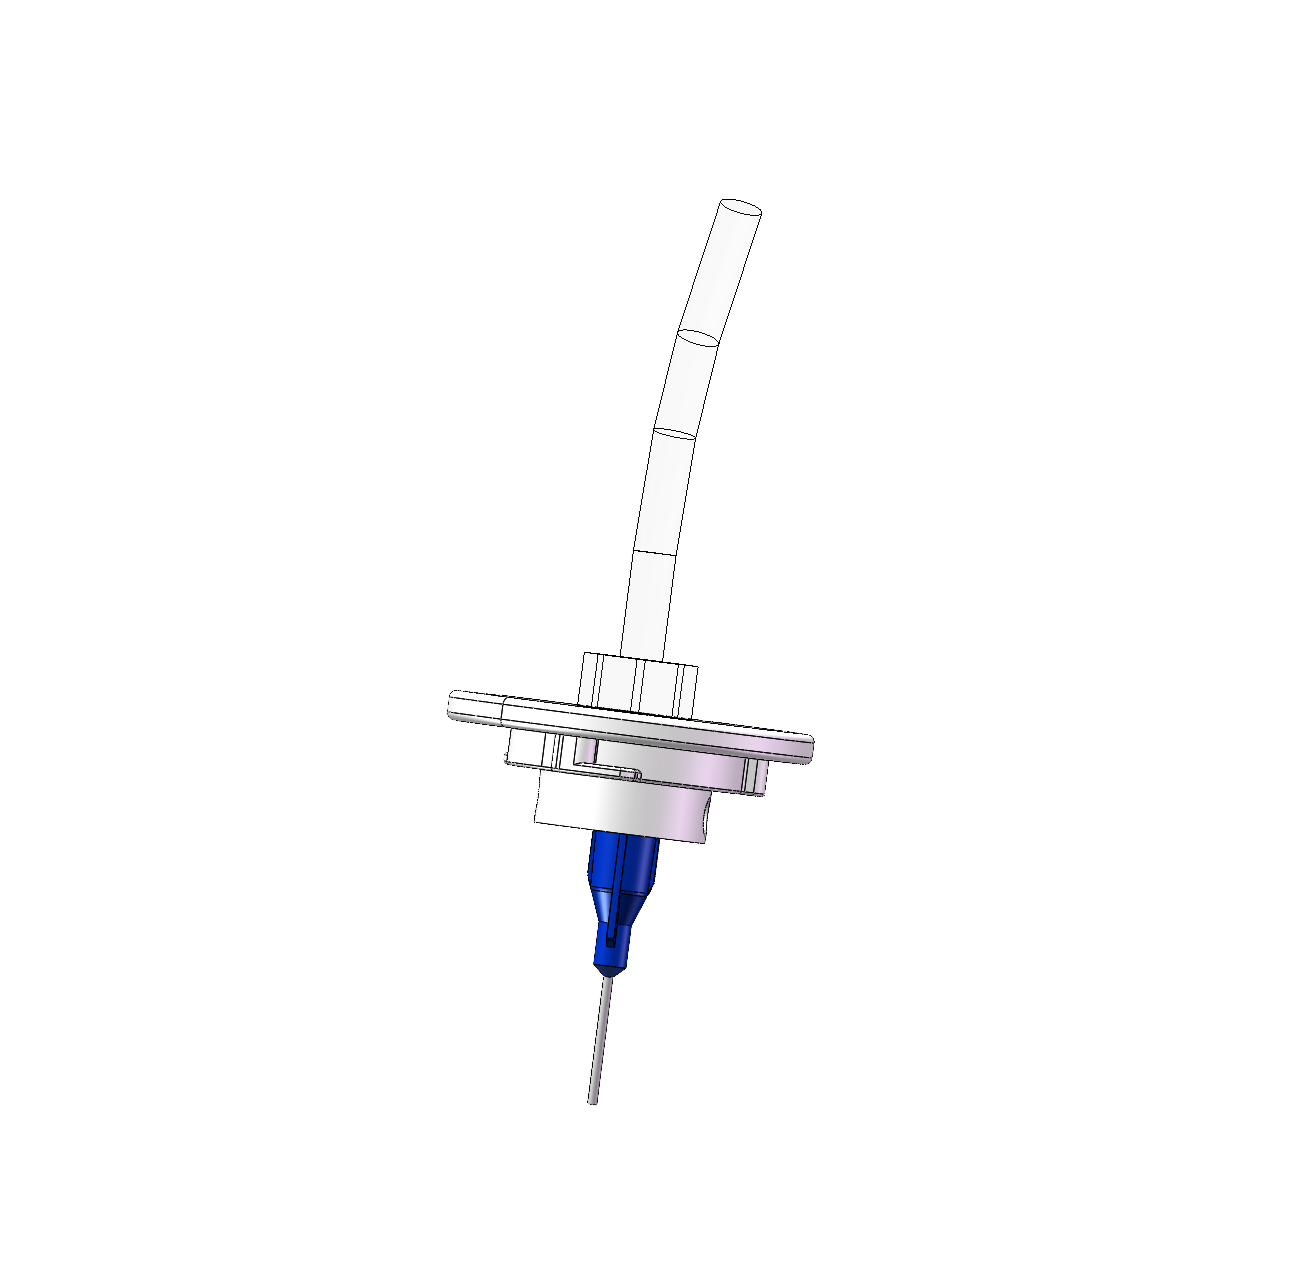
\includegraphics[width=\linewidth,height=4cm,keepaspectratio]{assets/img/针头.PNG}
    \caption{针头模块示意图}
    \label{fig:needle}
  \end{minipage}
  \hfill
  \begin{minipage}[t]{0.48\textwidth}
    \centering
    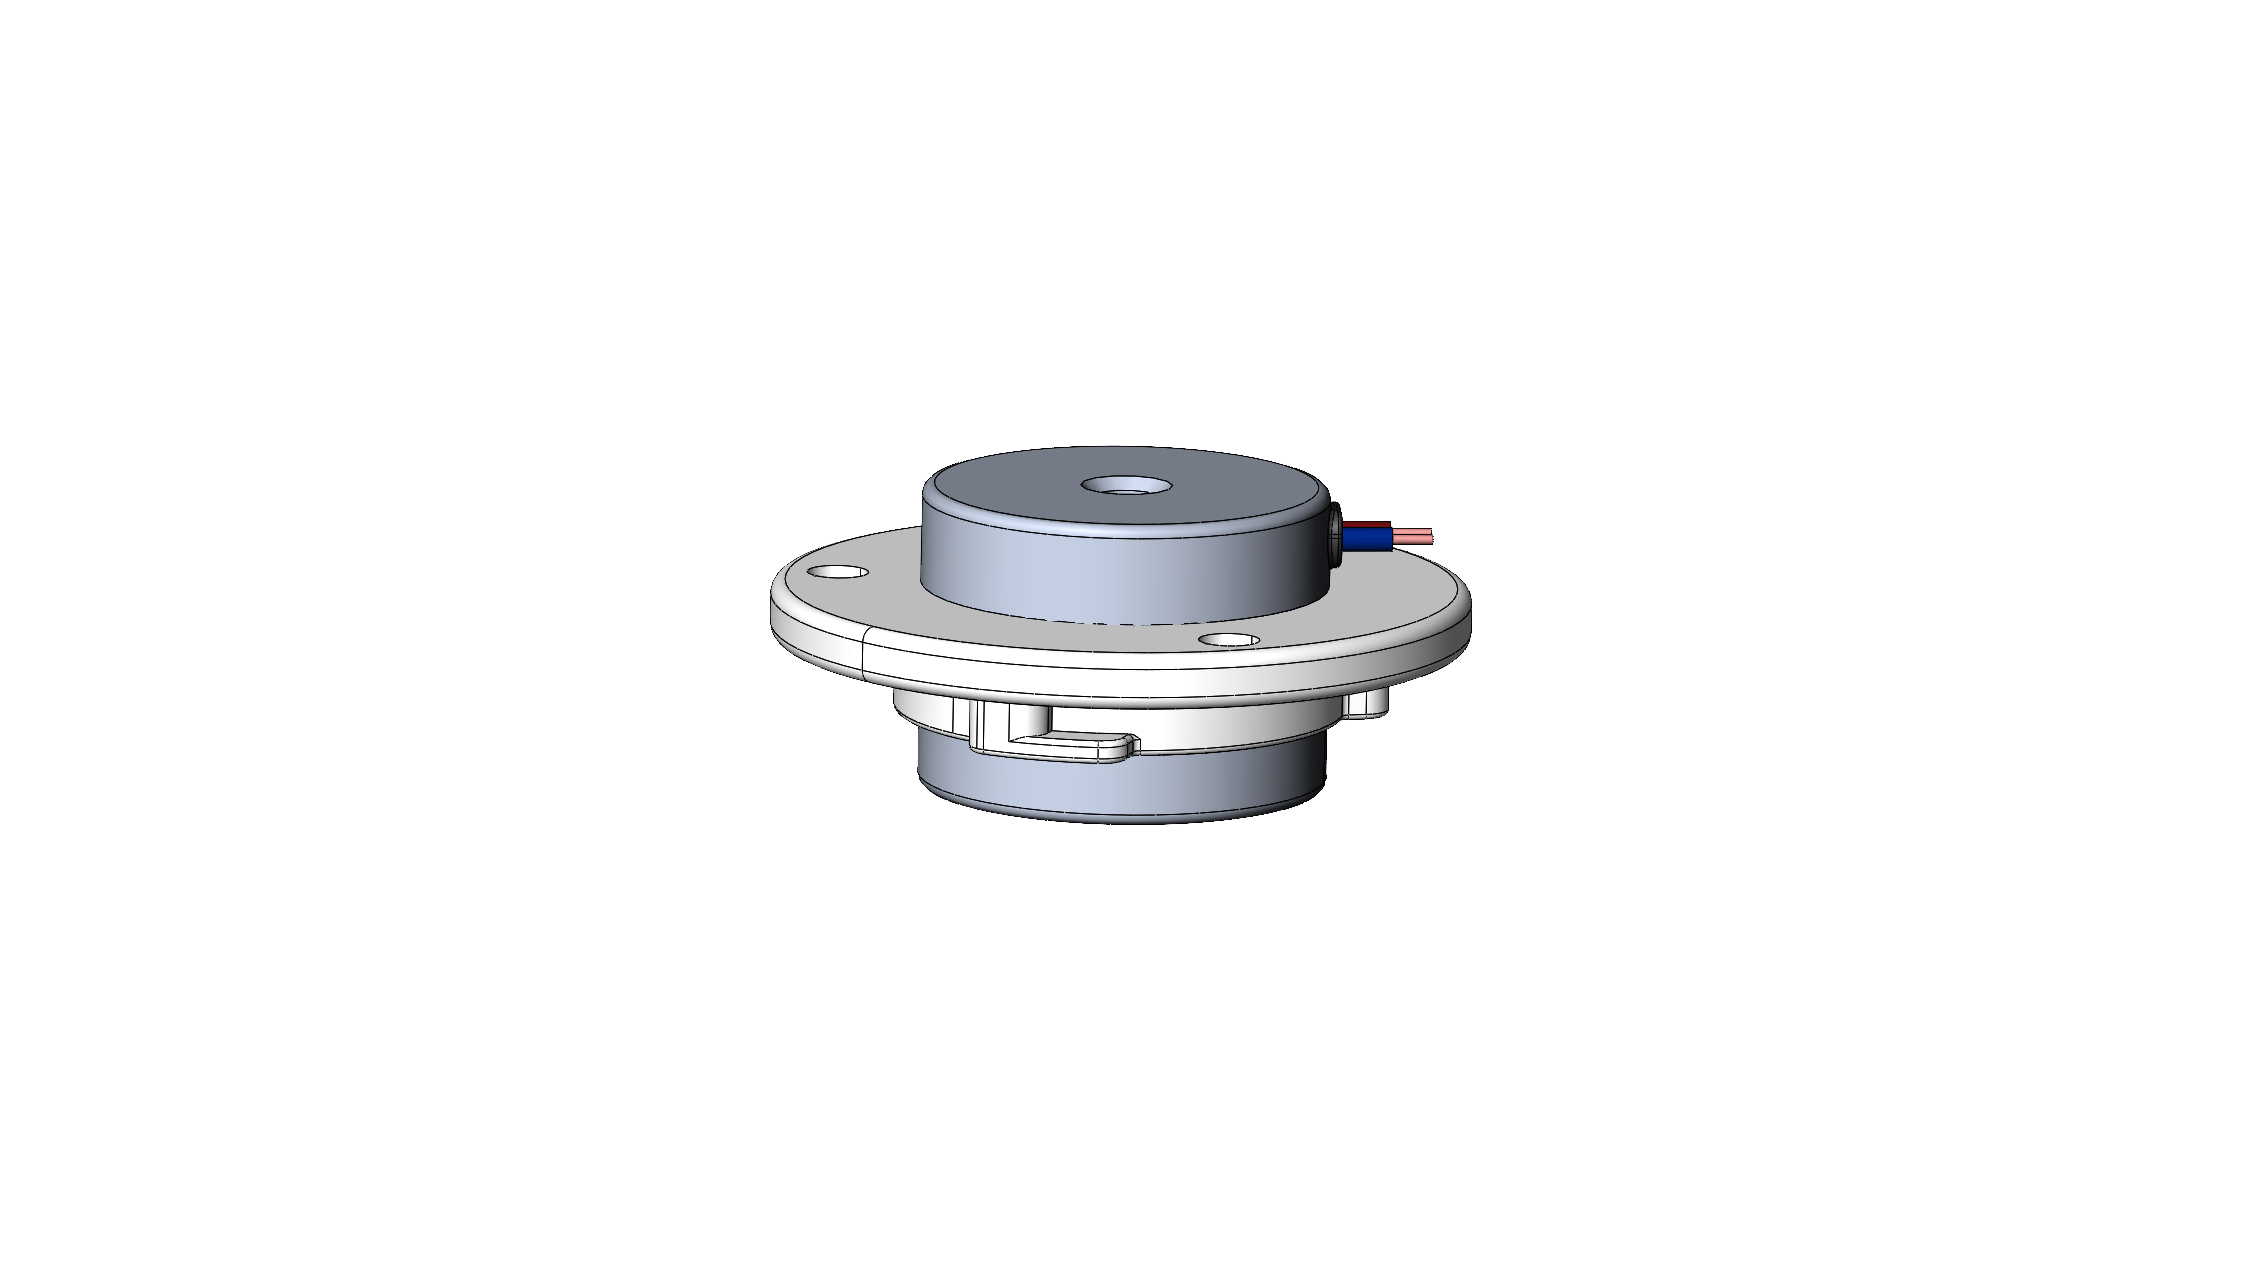
\includegraphics[width=\linewidth,height=4cm,keepaspectratio]{assets/img/电磁铁.PNG}
    \caption{电磁铁模块示意图}
    \label{fig:electromagnet}
  \end{minipage}

  \vspace{1em}

  \begin{minipage}[t]{0.48\textwidth}
    \centering
    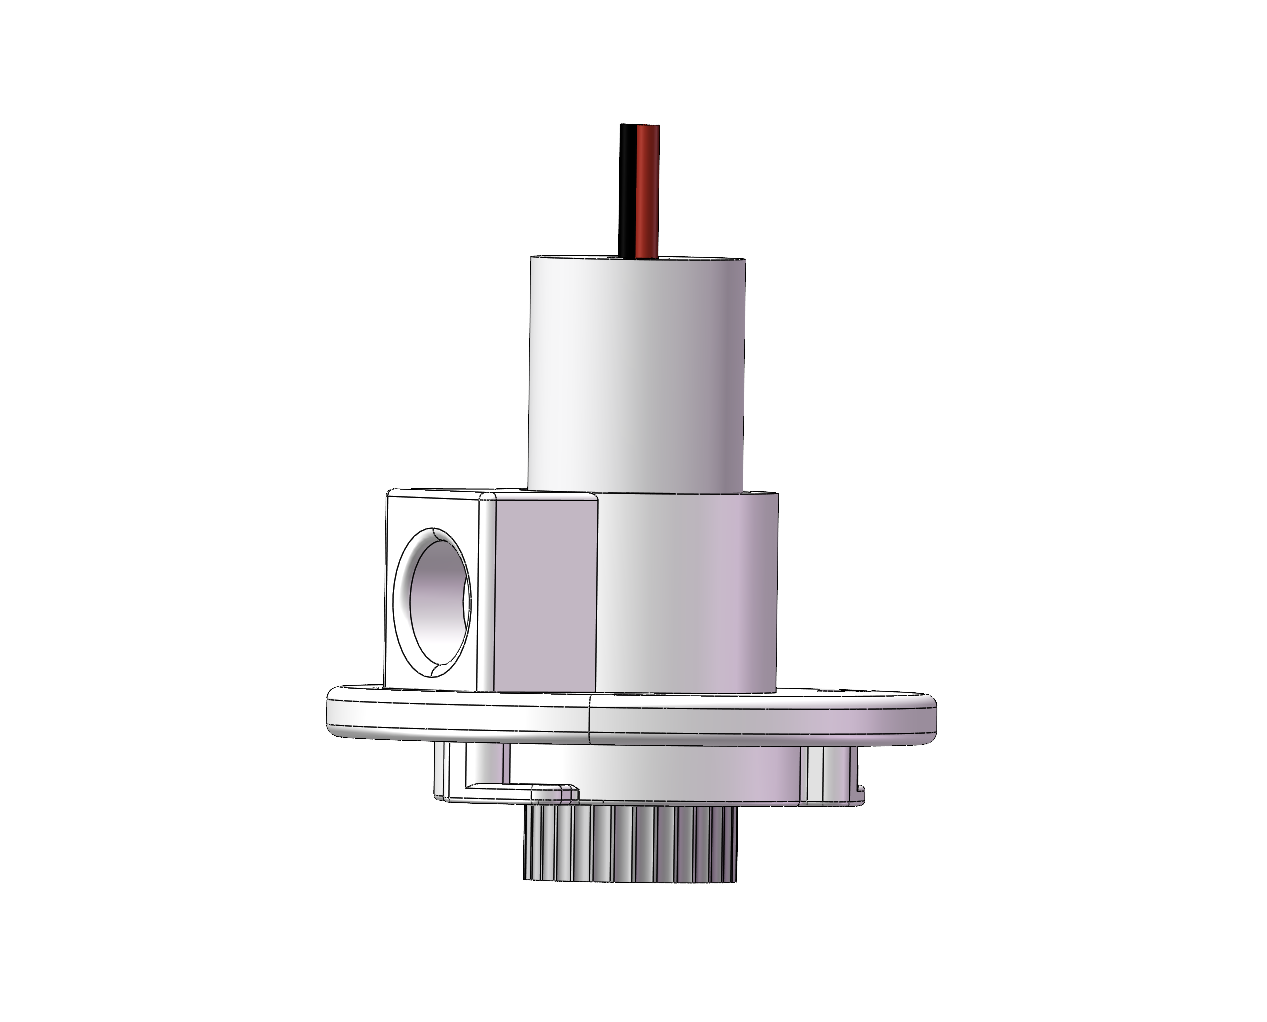
\includegraphics[width=\linewidth,height=4cm,keepaspectratio]{assets/img/激光.PNG}
    \caption{激光模块示意图}
    \label{fig:lasers}
  \end{minipage}
  \hfill
  \begin{minipage}[t]{0.48\textwidth}
    \centering
    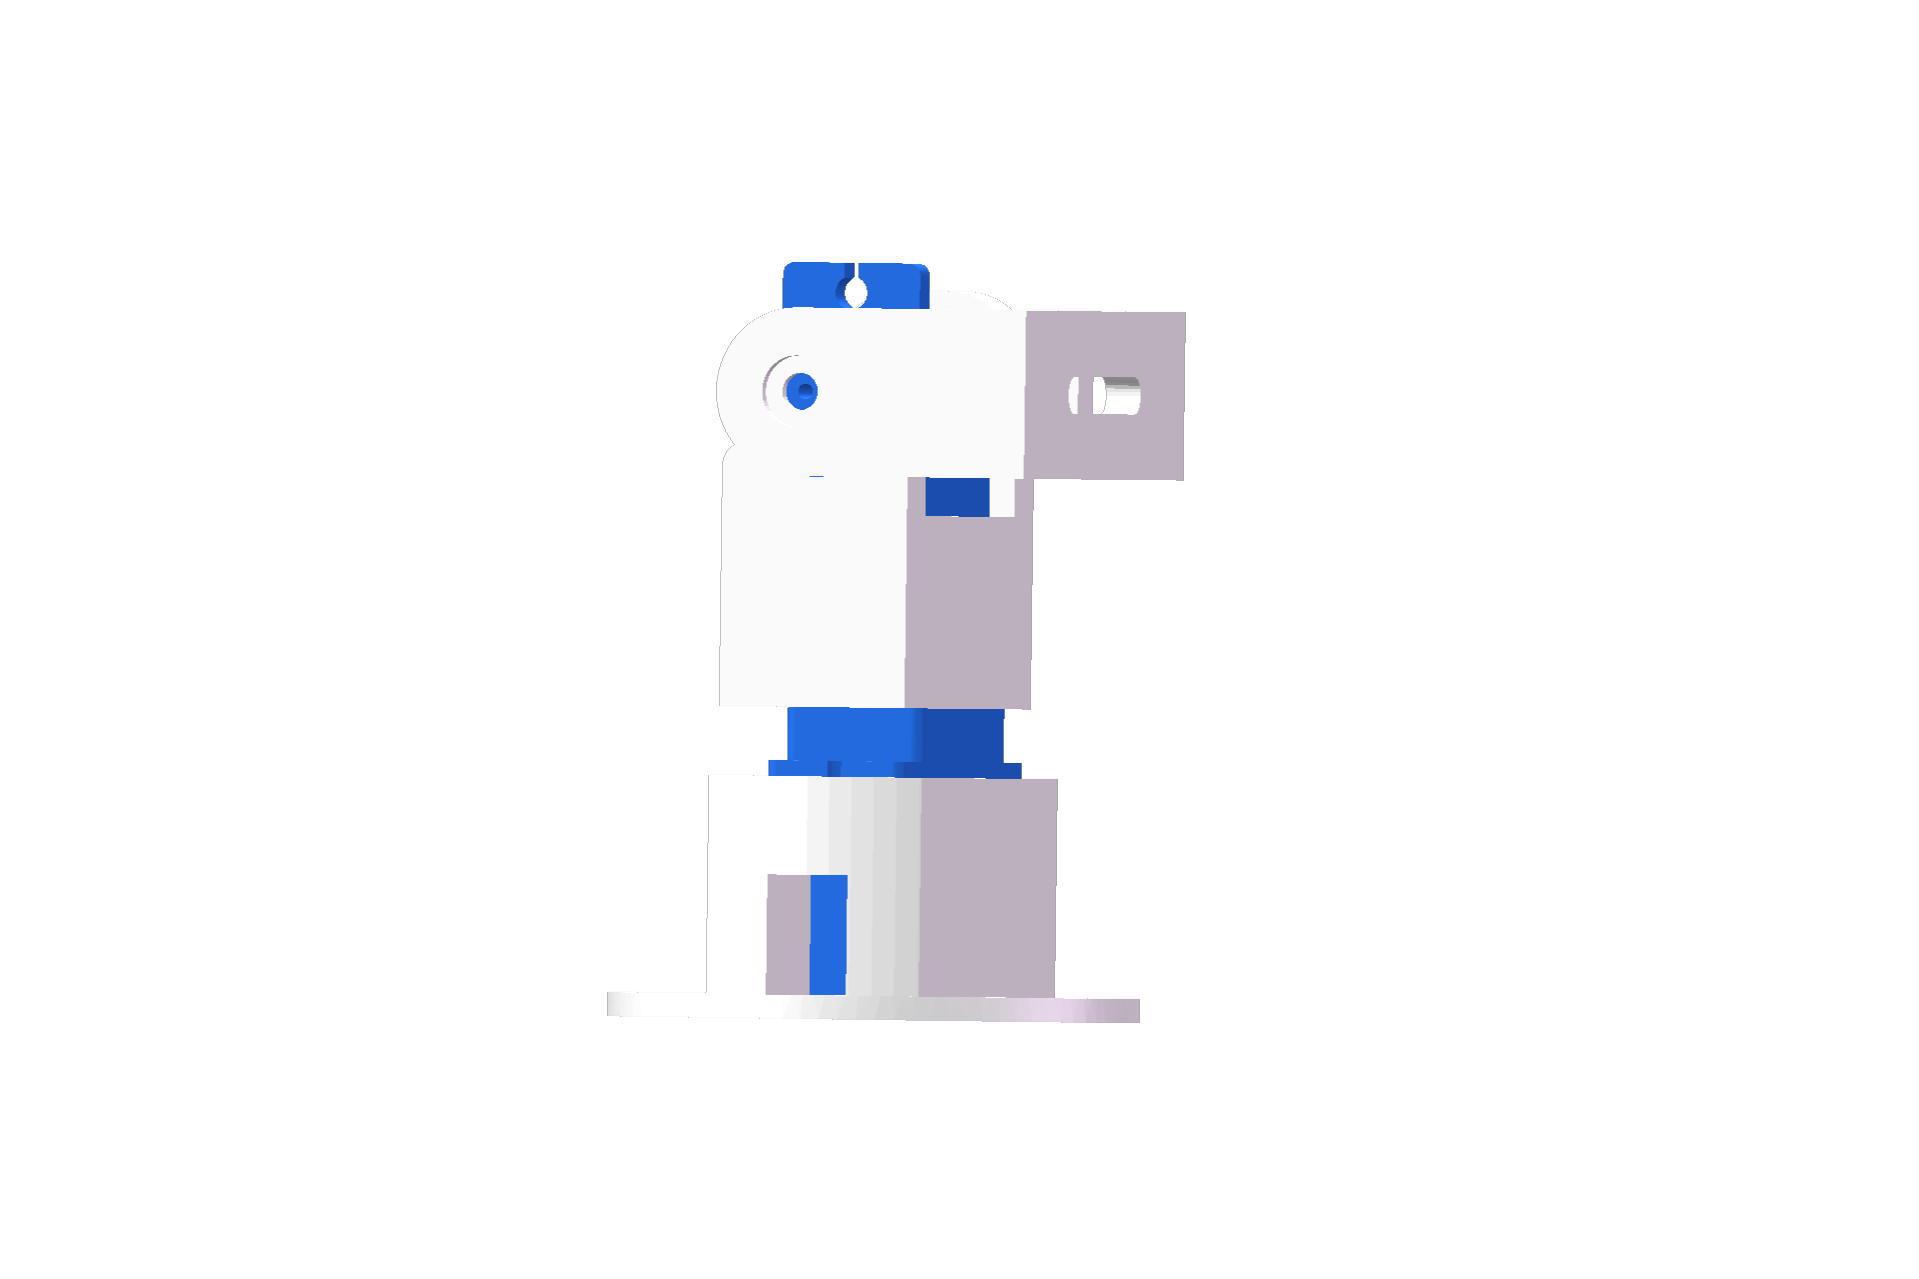
\includegraphics[width=\linewidth,height=4cm,keepaspectratio]{assets/img/舵机云台.PNG}
    \caption{舵机云台模块示意图}
    \label{fig:servo-gimbal}
  \end{minipage}
  \caption{四种末端执行器模块}
  \label{fig:end-effectors}
\end{figure}

\subsubsection{电路各模块介绍}
电路部分主要包括四个部分：电源模块、控制模块、驱动模块和传感器模块。各模块设计均围绕稳定供电、精确控制和可靠通信展开。
整体的电路原理图如图\ref{fig:circuit-overview}所示：
\begin{figure}[htbp]
  \centering
  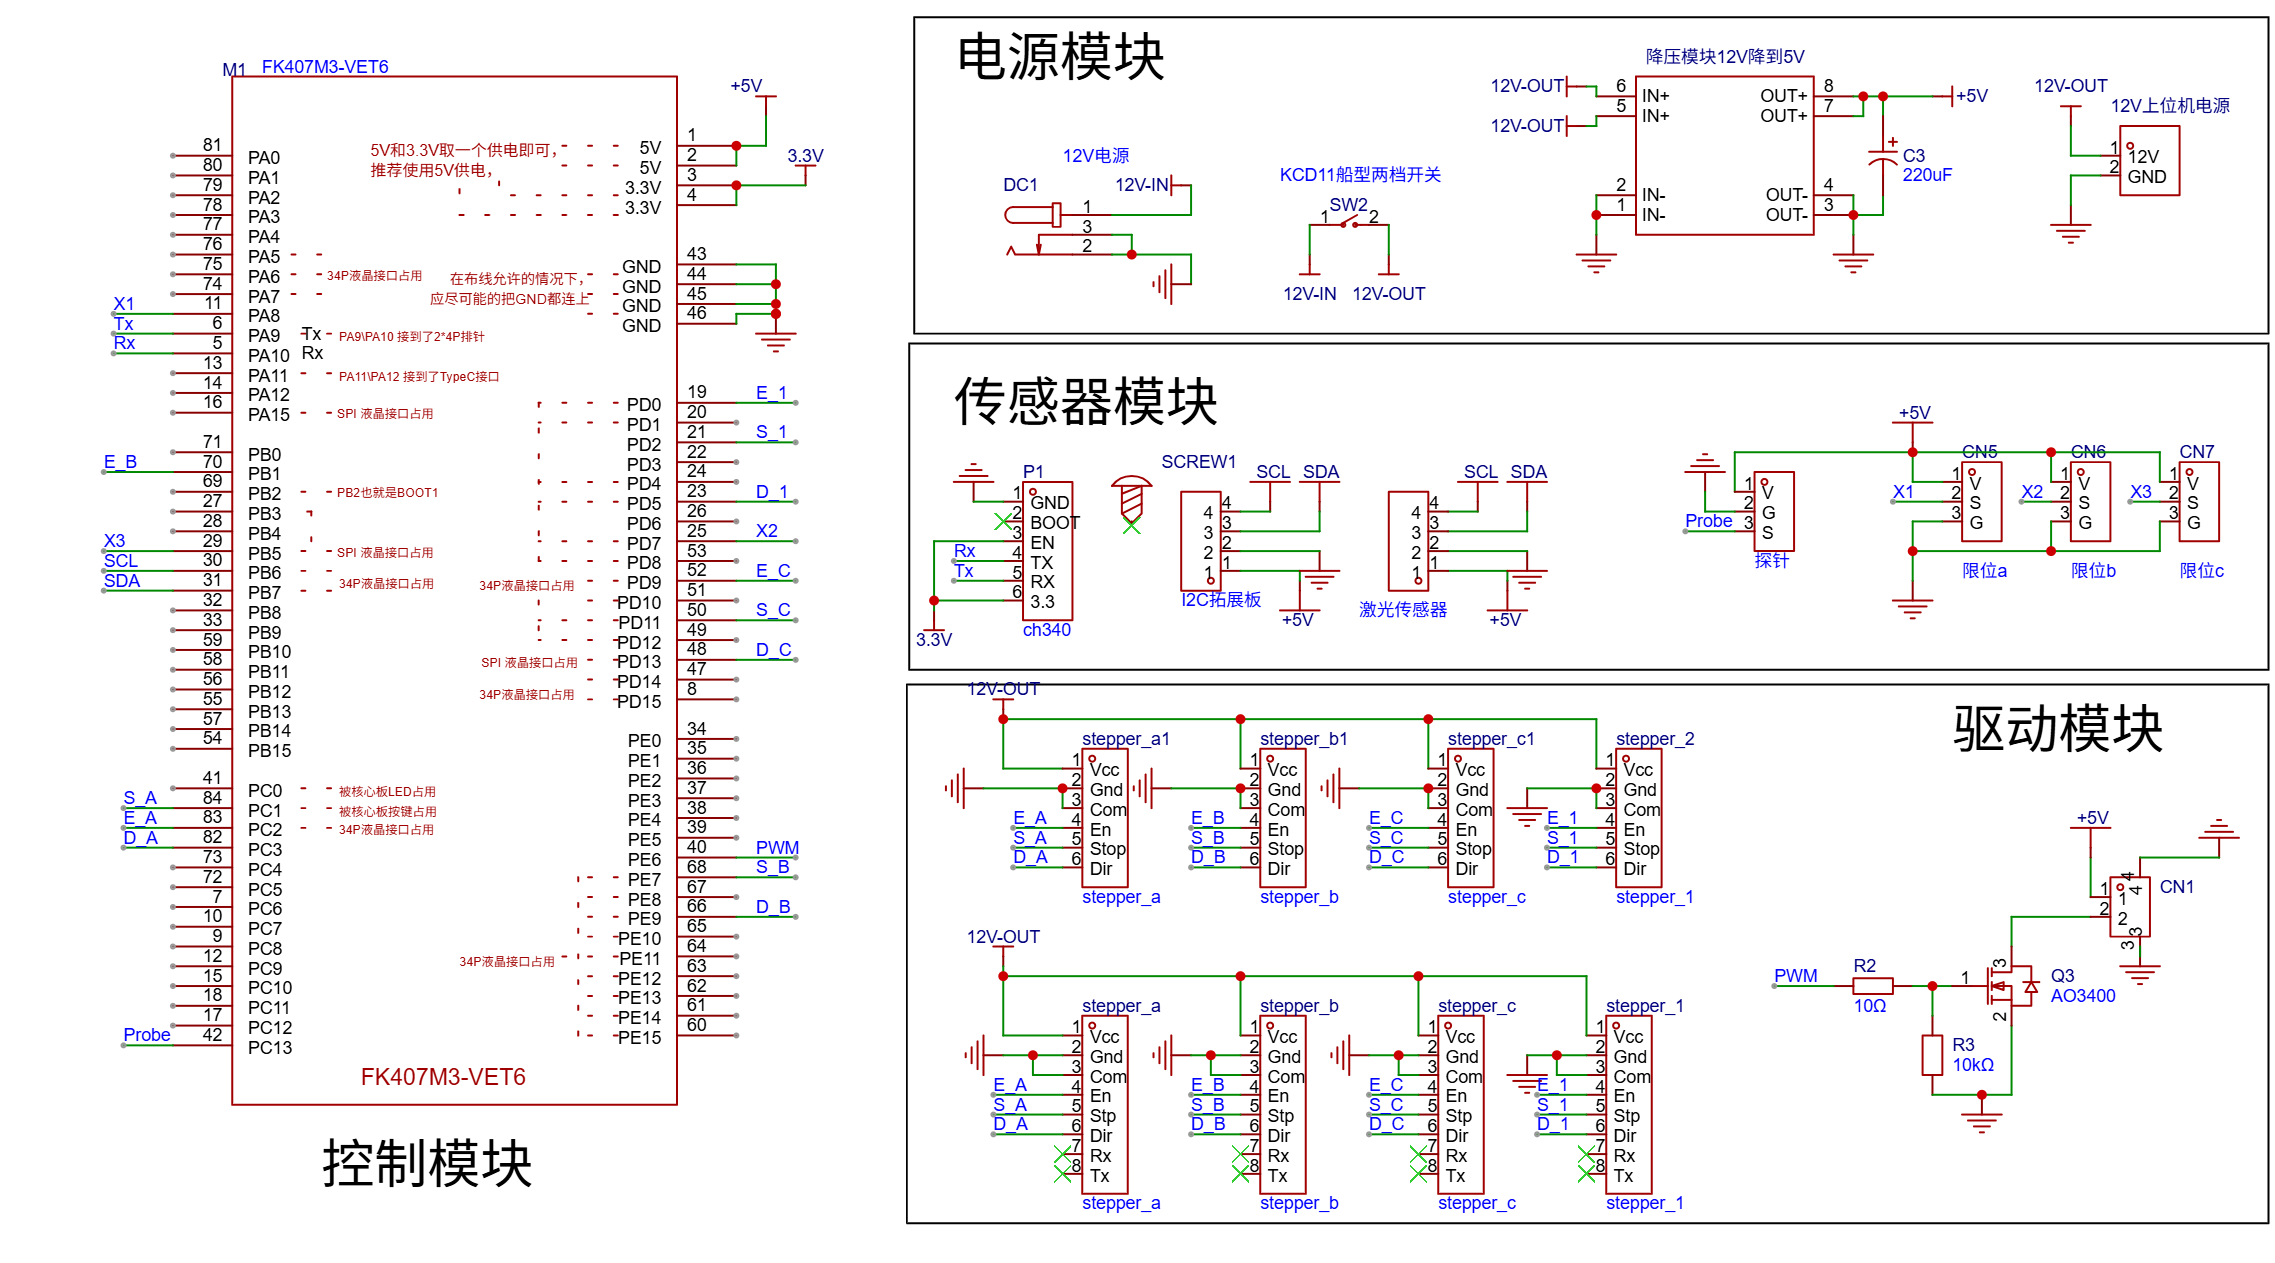
\includegraphics[width=0.9\textwidth,keepaspectratio]{assets/img/原理图.png}
  \caption{电路系统总体原理图}
  \label{fig:circuit-overview}
\end{figure}

\textbf{控制模块}：
控制模块的主体是 STM32F407VET6 微控制器，
它负责接收上位机的指令，进行运动学计算，并输出控制信号给驱动模块。
该模块还包括必要的接口电路，如 USB 接口、UART 接口和 GPIO 扩展，
以便与其他模块进行通信和控制。

\textbf{电源模块}：
电源模块负责为整个系统提供稳定的工作电压，确保各模块能够正常运行。
电源输入为 220\,V 交流市电，经适配器转换为 12\,V 直流电压，
12\,V 电压再通过降压电路（Mini 560）转换为 5\,V，为其他模块供电。

\textbf{传感器模块}：
本系统主要使用光电限位开关、摄像头模块和六轴姿态传感器等传感器模块。

光电限位开关：用于确定机械装置的归零点，为运动学解算提供一个基准点，其基本电路如图\ref{fig:led}所示；
六轴姿态传感器：用于检测上臂的姿态变化（尤其是旋转角度，该角度是运动学解算的主变量），辅助运动控制和误差补偿；
摄像头模块：用于采集工件图像，进行工件定位、曲面配准和高度估计，为轨迹补偿提供空间基准。

为满足下位机串口通信和摄像头图像采集的接口需求，系统设计了扩展坞电路，如图\ref{fig:dock-circuit}所示。该电路采用 CH334R 芯片，引出 4 路 USB 接口和 1 个 Type-C 接口。
\begin{figure}[htbp]
  \centering
  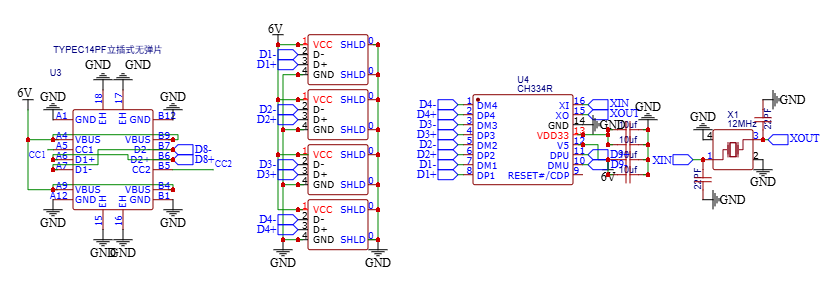
\includegraphics[width=0.9\textwidth,keepaspectratio]{assets/img/hub.png}
  \caption{拓展坞电路示意图}
  \label{fig:dock-circuit}
\end{figure}

\textbf{驱动模块}：
驱动模块主要包括步进电机驱动电路、激光/电磁铁驱动电路等。

步进电机驱动器支持脉冲控制与串口通信控制。本项目主要采用脉冲控制方式，驱动器接收来自 STM32F407 的 STEP/DIR/EN 信号，实现对步进电机的精确控制。
同时，STM32F407 通过串口与驱动器通信，获取步进电机的角度、位置和运行状态等信息。
为减少引脚资源占用，串口通信（USART）以及与六轴姿态传感器的通信（I2C）均采用“一主机多从机”架构。

激光/电磁铁驱动电路主要通过 PWM 信号控制 N 沟道 MOS 的开通与关断时间，实现激光头功率输出和电磁铁通断控制，两类负载可复用同类接口。
该设计可进一步实现激光书写或雕刻时的光强控制，以及物料拾取时的吸放控制。
其中驱动控制电路如图\ref{fig:laser-electromagnet}所示：
\begin{figure}[htbp]
  \centering
  \begin{minipage}[t]{0.48\textwidth}
    \centering
    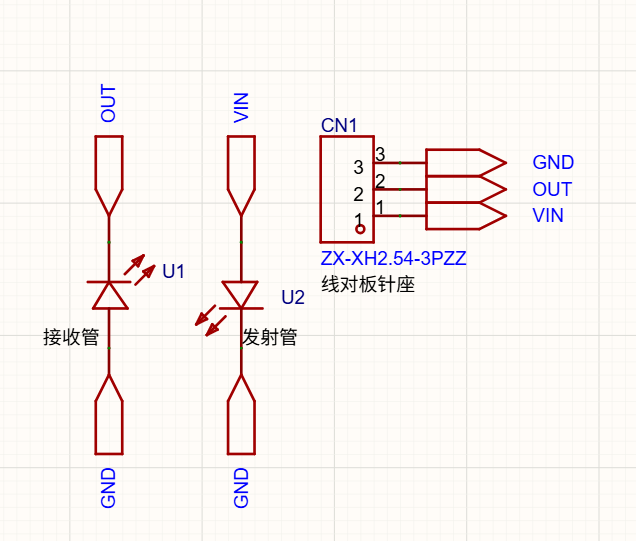
\includegraphics[width=\linewidth,keepaspectratio]{assets/img/光电对管.png}
    \caption{光电对管电路原理图}
    \label{fig:led}
  \end{minipage}
  \hfill
  \begin{minipage}[t]{0.48\textwidth}
    \centering
    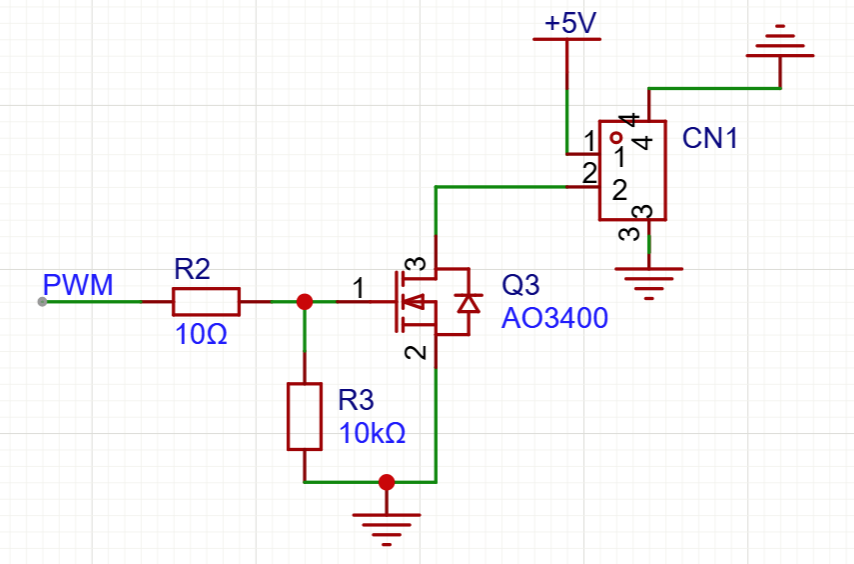
\includegraphics[width=\linewidth,keepaspectratio]{assets/img/驱动电路.png}
    \caption{激光/电磁铁驱动电路原理图}
    \label{fig:laser-electromagnet}
  \end{minipage}
\end{figure}

\subsection{软件系统介绍}

\subsubsection{软件整体介绍}
本项目的软件系统采用“上位机人机交互、主机通信与任务调度、下位机实时运动控制”的分层结构。

\begin{itemize}
  \item PC 端 Flutter 上位机负责提供控制面板、参数校准、曲面书写、激光加工和配置管理等主要操作界面；
  \item 机器人主机侧提供 HTTP 与 WebSocket 接口，承担状态汇总、G-code 脚本下发、文件管理、服务管理和任务执行调度；
  \item STM32F407 控制板运行实时运动固件，完成步进脉冲、PWM 输出、串口电机指令转发以及急停等时间敏感任务；
  \item 除 PC 上位机外，系统还保留本机触控屏显示程序，作为现场调试和脱机观察时的辅助交互入口。
\end{itemize}

\begin{figure}[htbp]
  \centering
  \resizebox{0.98\textwidth}{!}{%
  \begin{tikzpicture}[
    font=\small,
    >=Stealth,
    module/.style={draw, rounded corners=1.5mm, align=center, minimum height=9mm, inner sep=3pt, text width=30mm},
    page/.style={draw, rounded corners=1.2mm, align=center, minimum height=8mm, inner sep=2pt, text width=16mm, fill=cyan!10},
    layerlabel/.style={draw, rounded corners=1mm, align=center, font=\small\bfseries, minimum width=16mm, minimum height=12mm, inner sep=2pt, fill=white},
    ui/.style={module, fill=blue!10},
    gateway/.style={module, fill=green!10},
    host/.style={module, fill=orange!12},
    realtime/.style={module, fill=red!10},
    hw/.style={module, fill=gray!12},
    arrow/.style={->, thick, rounded corners=1.5mm},
    flow/.style={thick, rounded corners=1.5mm},
    feedback/.style={->, dashed, thick, rounded corners=1.5mm},
    layer/.style={draw, rounded corners=2mm, densely dotted, inner sep=6pt, fill=#1, fill opacity=0.08, text opacity=1}
  ]
    \node[layerlabel, fill=blue!12] (labelui) at (-6.35,6.0) {交互\\业务};
    \node[ui] (touch) at (-3.9,7.25) {本机触控屏\\现场辅助操作};
    \node[ui] (pc) at (0,7.25) {Flutter 上位机\\界面与状态管理};
    \node[ui] (state) at (3.9,7.25) {状态控制器\\导航与数据缓存};

    \node[page] (control) at (-4.6,5.95) {控制\\面板};
    \node[page] (calib) at (-2.3,5.95) {参数\\校准};
    \node[page] (surface) at (0,5.95) {曲面};
    \node[page] (laserpg) at (2.3,5.95) {激光};
    \node[page] (config) at (4.6,5.95) {配置};
    \node[ui, text width=42mm] (controller) at (0,4.65) {业务控制器\\命令封装与状态分发};

    \node[layerlabel, fill=green!12] (labelcomm) at (-6.35,3.0) {通信\\主机};
    \node[gateway] (moon) at (-3.9,3.0) {Moonraker\\REST / WebSocket};
    \node[gateway] (filecfg) at (0,3.0) {文件、配置与任务\\上传 / 编辑 / 启动};
    \node[gateway] (vision) at (3.9,3.0) {相机服务与视觉脚本\\快照 / 标定 / 验证};

    \node[layerlabel, fill=orange!14] (labelctrl) at (-6.35,1.0) {实时\\控制};
    \node[host] (motion) at (-3.9,1.0) {主机运动服务\\队列执行与状态广播};
    \node[realtime] (mcu) at (0,1.0) {STM32F407 实时固件\\命令解析与事件调度};
    \node[realtime] (emm) at (3.9,1.0) {电机串口扩展\\回零 / 读位置 / 轨迹播放};

    \node[layerlabel, fill=gray!18] (labelhw) at (-6.35,-1.05) {执行\\感知};
    \node[hw] (motors) at (-3.9,-1.05) {闭环步进驱动器\\Delta 机构};
    \node[hw] (laserhw) at (0,-1.05) {激光器\\PWM 功率输出};
    \node[hw] (camera) at (3.9,-1.05) {摄像头\\工件图像};

    \draw[arrow] (touch.east) -- (pc.west);
    \draw[arrow] (pc.east) -- (state.west);
    \draw[arrow] (pc.south) -- (surface.north);
    \foreach \n in {control,calib,surface,laserpg,config} {
      \draw[arrow] (\n.south) -- ++(0,-0.25) |- (controller.north);
    }

    \coordinate (commbus) at (0,3.85);
    \draw[flow] (controller.south) -- (commbus);
    \draw[arrow] (commbus) -| (moon.north);
    \draw[arrow] (commbus) -- (filecfg.north);
    \draw[arrow] (commbus) -| (vision.north);

    \draw[arrow] (moon.south) -- (motion.north);
    \draw[arrow] (filecfg.south) -- ++(0,-0.38) -| (motion.north);
    \draw[arrow] (vision.south) -- ++(0,-0.38) -| (motion.north);

    \draw[arrow] (motion.east) -- (mcu.west);
    \draw[arrow] (mcu.east) -- (emm.west);
    \draw[arrow] (mcu.south) -- (laserhw.north);
    \draw[arrow] (mcu.south west) -- ++(-0.7,-0.45) -| (motors.north east);
    \draw[arrow] (emm.south) -- ++(0,-0.65) -| (motors.north);

    \draw[feedback] ([xshift=-3mm]motion.north) -- ([xshift=-3mm]moon.south);
    \draw[feedback] ([xshift=-3mm]moon.north) -- ++(0,1.22) -- (controller.west);
    \draw[feedback] (camera.east) -- ++(0.65,0) |- (vision.east);

    \begin{scope}[on background layer]
      \node[layer=blue!30, fit=(labelui)(touch)(pc)(state)(control)(calib)(surface)(laserpg)(config)(controller)] {};
      \node[layer=green!30, fit=(labelcomm)(moon)(filecfg)(vision)] {};
      \node[layer=orange!35, fit=(labelctrl)(motion)(mcu)(emm)] {};
      \node[layer=gray!35, fit=(labelhw)(motors)(laserhw)(camera)] {};
    \end{scope}
    \node[draw, rounded corners=1mm, fill=white, align=center, font=\footnotesize, inner sep=3pt, text width=120mm]
      (legend) at (0,-2.35) {实线：控制命令、任务文件与运动指令下发 \qquad 虚线：状态、图像与计算结果反馈};
  \end{tikzpicture}%
  }
  \caption{软件各模块总体关系框架图}
  \label{fig:software_module_framework}
\end{figure}

图 \ref{fig:software_module_framework} 给出了软件系统各模块之间的整体关系。实线表示控制命令、任务文件或运动指令的下发路径，虚线表示状态、图像或计算结果的反馈路径。

从运行流程看，用户首先在连接界面输入主机 IP、端口，PC 上位机据此建立 HTTP 连接并打开 WebSocket 长连接。HTTP 通道主要用于获取服务信息、上传或删除 G-code 文件、启动任务、读写配置文件和调用服务重启接口；WebSocket 通道用于订阅任务状态、运动坐标、文件进度、外设状态等实时数据，并将这些数据更新到界面控制器中。用户在界面上发出的回零、点动、激光开关、曲面扫描、轨迹上传等操作最终被转化为 G-code 脚本或文件任务，经主机服务下发到底层运动控制程序。

主机侧软件在系统中起到“协议网关”和“任务中枢”的作用：
\begin{itemize}
  \item 向 PC 上位机和本机触控屏暴露统一的 REST 与 WebSocket 接口；
  \item 根据配置文件中的机构参数、电机引脚、激光 PWM 引脚和扩展模块设置，将高层命令转换为底层控制板能够执行的动作。
\end{itemize}

对于机器人书写任务，G-code 文件可由上位机直接生成并上传，也可以由主机的任务文件界面加载执行。

对于视觉标定和曲面电路喷印，Flutter 上位机还会调用本地 Python 标定脚本和图像检测脚本，完成图像采集、坐标变换求解、误差采样、曲面轨迹修正和验证。

下位机 STM32F407 固件负责所有对实时性要求高的动作。
其主循环由系统时钟初始化、命令收发、任务调度、定时器事件和外设驱动组成。
主机下发的配置命令首先分配对象并绑定 GPIO、定时器、串口等资源，运动开始后，固件按照规划好的时间点触发步进输出或 PWM 更新，保证电机动作和激光开关具有确定的时序。
针对本项目闭环步进电机驱动器，还增加了基于 USART2 的电机串口通信模块，用于发送使能、清零、读位置、回零等指令，使三组关节电机的状态能够被主机侧扩展模块读取和校验。

\begin{table}[htbp]
  \centering
  \small
  \renewcommand{\arraystretch}{1.25}
  \begin{tabular}{|p{0.18\linewidth}|p{0.33\linewidth}|p{0.39\linewidth}|}
    \hline
    软件层级 & 主要组成 & 功能说明 \\
    \hline
    PC 上位机 & Flutter 应用、状态控制器、页面组件、文件与轨迹生成模块 & 提供人机交互界面，完成连接管理、手动控制、参数校准、曲面轨迹生成、激光加工路径生成和配置文件编辑。 \\
    \hline
    本机辅助交互 & 触控屏显示程序、屏幕 WebSocket 客户端、屏幕 REST 客户端 & 在机器人本机屏幕上显示状态、任务和控制页面，可独立完成基础控制、任务观察和服务重启。 \\
    \hline
    主机通信与调度 & REST 接口、WebSocket 订阅、文件管理、G-code 执行、相机服务 & 汇总设备状态和运动状态，接收上位机命令，管理配置文件和 G-code 文件，并为视觉标定提供相机图像接口。 \\
    \hline
    实时控制层 & STM32F407 固件、步进输出、PWM 输出、USART2 电机串口扩展 & 执行实时运动控制、激光 PWM 控制和闭环步进驱动器串口通信。 \\
    \hline
  \end{tabular}
  \caption{软件系统分层及功能划分}
  \label{tab:software_layers}
\end{table}

软件整体数据流可概括为：上位机界面接收用户意图，控制器将其封装为 HTTP 请求、WebSocket 订阅或 G-code 脚本；
主机服务接收后进行任务排队、状态广播和配置解析；
实时固件根据主机下发的命令驱动电机、激光和外设；
执行结果再经状态订阅通道返回界面显示。
该结构将界面交互、网络通信、视觉计算和实时控制分离，既便于在 PC 端快速迭代复杂功能，也保证了底层运动控制的稳定性和实时性。

\subsubsection{软件各模块介绍}
基于图 \ref{fig:software_module_framework} 中的分层关系，后续各模块说明按照交互与业务层、通信与主机服务层、实时控制层和执行与感知外设的顺序展开。
\paragraph{上位机连接与状态管理模块}
上位机连接与状态管理模块负责将用户输入的主机地址、连接参数和控制命令转换为统一的通信配置、状态订阅和业务调用。程序入口通过 Provider 注册设备状态、导航、纸张配置、参数校准、相机和字体等控制器；连接页面读取主机 IP、端口、协议和 API Key 后初始化通信控制器。连接界面如图 \ref{fig:connect} 所示，完整连接流程如图 \ref{fig:pc_connection_flow} 所示。

\begin{figure}[htbp]
  \centering
  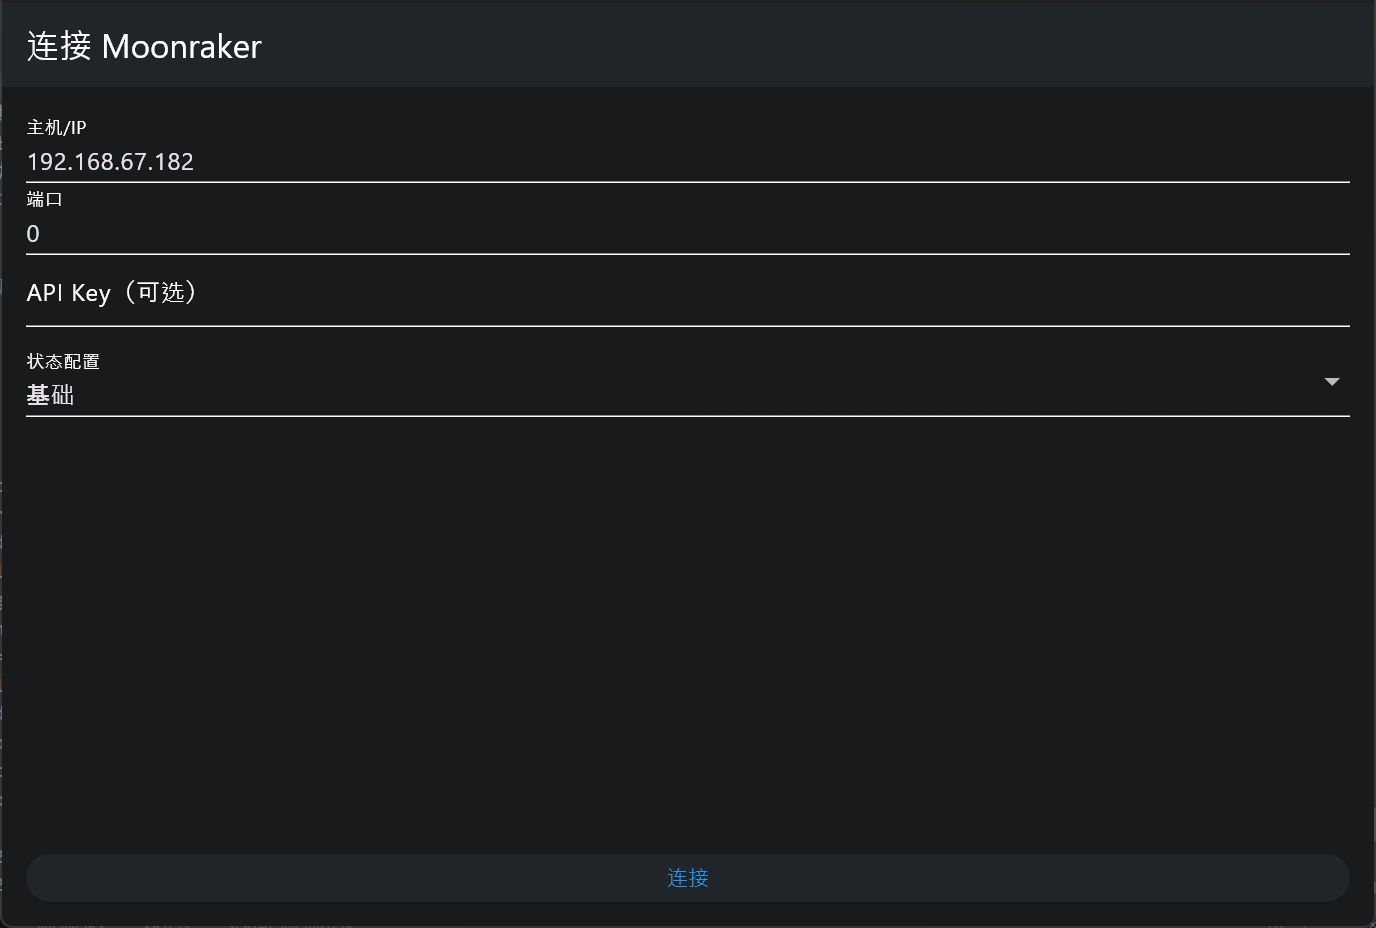
\includegraphics[width=0.6\textwidth,keepaspectratio]{assets/img/连接界面.png}
  \caption{软件连接界面图}
  \label{fig:connect}
\end{figure}
\begin{figure}[htbp]
  \centering
  \resizebox{0.96\textwidth}{!}{%
  \begin{tikzpicture}[
    font=\small,
    >=Stealth,
    flowbox/.style={draw, rounded corners=1.5mm, align=center, minimum height=9mm, inner sep=3pt, text width=27mm, fill=blue!8},
    servicebox/.style={flowbox, fill=green!10},
    statebox/.style={flowbox, fill=orange!12},
    inputbox/.style={flowbox, fill=cyan!10},
    decisionbox/.style={draw, diamond, aspect=2.1, align=center, inner sep=1pt, text width=19mm, fill=yellow!15},
    arrow/.style={->, thick, rounded corners=1.5mm},
    feedback/.style={->, dashed, thick, rounded corners=1.5mm}
  ]
    \node[inputbox] (input) at (0,2.2) {连接页面\\IP / 端口 / API Key};
    \node[flowbox] (config) at (3.4,2.2) {生成通信配置\\初始化控制器};
    \node[servicebox] (http) at (6.8,2.2) {HTTP 请求\\服务与设备信息};
    \node[decisionbox] (ok) at (10.0,2.2) {连接\\成功?};
    \node[servicebox] (ws) at (14.05,2.2) {建立 WebSocket\\长连接};
    \node[statebox] (subscribe) at (14.05,0.55) {订阅状态对象\\坐标 / 任务 / 文件};
    \node[statebox] (refresh) at (9.6,0.55) {接收状态包\\通知界面刷新};
    \node[flowbox] (home) at (6.2,0.55) {进入主页面\\响应用户操作};
    \node[servicebox] (command) at (2.8,0.55) {封装命令\\HTTP / G-code / 文件任务};
    \node[statebox] (retry) at (10.0,-1.05) {记录错误\\递增延时重连};

    \draw[arrow] (input.east) -- (config.west);
    \draw[arrow] (config.east) -- (http.west);
    \draw[arrow] (http.east) -- (ok.west);
    \draw[arrow] (ok.east) -- node[above, font=\footnotesize] {是} (ws.west);
    \draw[arrow] (ws.south) -- (subscribe.north);
    \draw[arrow] (subscribe.west) -- (refresh.east);
    \draw[arrow] (refresh.west) -- (home.east);
    \draw[arrow] (home.west) -- (command.east);
    \draw[arrow] (command.north) |- (http.south);

    \draw[feedback] (ok.south) -- node[pos=0.86, right, font=\footnotesize] {否} (retry.north);
    \draw[feedback] (retry.west) -- ++(-8.75,0) |- (input.south);
  \end{tikzpicture}%
  }
  \caption{上位机连接与状态订阅流程图}
  \label{fig:pc_connection_flow}
\end{figure}

\paragraph{Moonraker 无线通信模块}
无线通信模块的主要交互如图~\ref{fig:moonraker_wireless_sequence} 所示。HTTP 通道负责服务查询、G-code 下发、文件上传和任务启动等一次性请求，WebSocket 通道负责对象状态订阅和实时通知。通信仓库层把两类通道封装为连接、发送指令、上传并执行等业务接口，使界面层只需要处理用户操作和状态刷新。

\begin{figure}[htbp]
  \centering
  \resizebox{\textwidth}{!}{%
  \begin{tikzpicture}[
    font=\footnotesize,
    >=Stealth,
    actor/.style={draw, rounded corners=1.5mm, align=center, minimum width=23mm, minimum height=8mm, inner sep=2pt, fill=#1},
    actor/.default=blue!8,
    lifeline/.style={densely dashed, gray!65},
    msg/.style={->, thick},
    ret/.style={->, dashed, thick, gray!75},
    lab/.style={font=\scriptsize, align=center, fill=white, text=black, inner sep=1pt},
    bandlabel/.style={font=\scriptsize\bfseries, anchor=west, align=left}
  ]
    \begin{scope}[on background layer]
      \filldraw[fill=blue!6, draw=blue!30, rounded corners=1mm] (-1.70,-0.55) rectangle (13.15,-3.05);
      \filldraw[fill=green!6, draw=green!35, rounded corners=1mm] (-1.70,-3.30) rectangle (13.15,-4.85);
      \filldraw[fill=orange!8, draw=orange!40, rounded corners=1mm] (-1.70,-5.10) rectangle (13.15,-7.85);
    \end{scope}

    \node[actor=blue!10] (ctrl) at (0,0) {Flutter\\业务控制器};
    \node[actor=green!10] (http) at (3,0) {HTTP\\服务封装};
    \node[actor=cyan!10] (ws) at (6,0) {WebSocket\\服务封装};
    \node[actor=orange!12] (moon) at (9,0) {Moonraker\\主机服务};
    \node[actor=red!10] (klippy) at (12,0) {STM32\\与文件系统};

    \foreach \x in {0,3,6,9,12} {
      \draw[lifeline] (\x,-0.45) -- (\x,-8.05);
    }

    \node[bandlabel] at (-1.60,-0.82) {状态订阅};
    \draw[msg] (0,-1.12) -- node[lab, above] {发起连接} (3,-1.12);
    \draw[msg] (3,-1.42) -- node[lab, above] {GET \texttt{/server/info}\\GET \texttt{/printer/info}} (9,-1.42);
    \draw[ret] (9,-1.72) -- node[lab, above] {JSON 基本信息} (3,-1.72);
    \draw[msg] (0,-2.05) -- node[lab, above] {构造订阅对象} (6,-2.05);
    \draw[msg] (6,-2.35) -- node[lab, above] {JSON-RPC \texttt{printer.objects.subscribe}} (9,-2.35);
    \draw[ret] (9,-2.65) -- node[lab, above] {\texttt{notify\_status\_update}} (6,-2.65);
    \draw[ret] (6,-2.92) -- node[lab, above] {坐标、进度、\texttt{emm\_uart} 状态} (0,-2.92);

    \node[bandlabel] at (-1.60,-3.57) {即时 G-code};
    \draw[msg] (0,-3.88) -- node[lab, above] {\texttt{sendGcode(script)}} (3,-3.88);
    \draw[msg] (3,-4.18) -- node[lab, above] {POST \texttt{/printer/gcode/script}} (9,-4.18);
    \draw[msg] (9,-4.48) -- node[lab, above] {解析并排队执行} (12,-4.48);
    \draw[ret] (12,-4.72) -- node[lab, above] {响应与状态变化} (9,-4.72);

    \node[bandlabel] at (-1.60,-5.37) {上传并启动任务};
    \draw[msg] (0,-5.68) -- node[lab, above] {\texttt{uploadGcode}} (3,-5.68);
    \draw[msg] (3,-5.98) -- node[lab, above] {POST \texttt{/server/files/upload}} (9,-5.98);
    \draw[msg] (9,-6.28) -- node[lab, above] {保存到 \texttt{gcodes}} (12,-6.28);
    \draw[msg] (0,-6.68) -- node[lab, above] {\texttt{startPrintUploaded}} (3,-6.68);
    \draw[msg] (3,-6.98) -- node[lab, above] {POST \texttt{/printer/print/start}} (9,-6.98);
    \draw[msg] (9,-7.28) -- node[lab, above] {读取并执行文件} (12,-7.28);
    \draw[ret] (9,-7.58) -- node[lab, above] {任务进度通知} (6,-7.58);
  \end{tikzpicture}%
  }
  \caption{Moonraker 无线通信时序图}
  \label{fig:moonraker_wireless_sequence}
\end{figure}

\paragraph{控制面板模块}
控制面板是日常调试和执行任务的中心页面，主要由状态面板、运动控制面板、激光控制面板、相机面板、控制台和任务面板组成。
状态面板显示实时坐标和设备连接状态，并支持输入绝对坐标后发送 \texttt{G90} 与 \texttt{G1} 指令移动到指定位置。运动控制面板提供步长选择、XYZ 点动、单轴回零和全轴回零功能，点动命令采用相对坐标模式发送，回零命令则根据用户选择生成对应轴的 \texttt{G28} 命令。

控制台允许用户直接输入 G-code，便于调试单条命令；任务面板则读取主机文件列表，显示当前任务进度，并支持删除文件和启动指定 G-code 文件。
\begin{figure}[htbp]
  \centering
  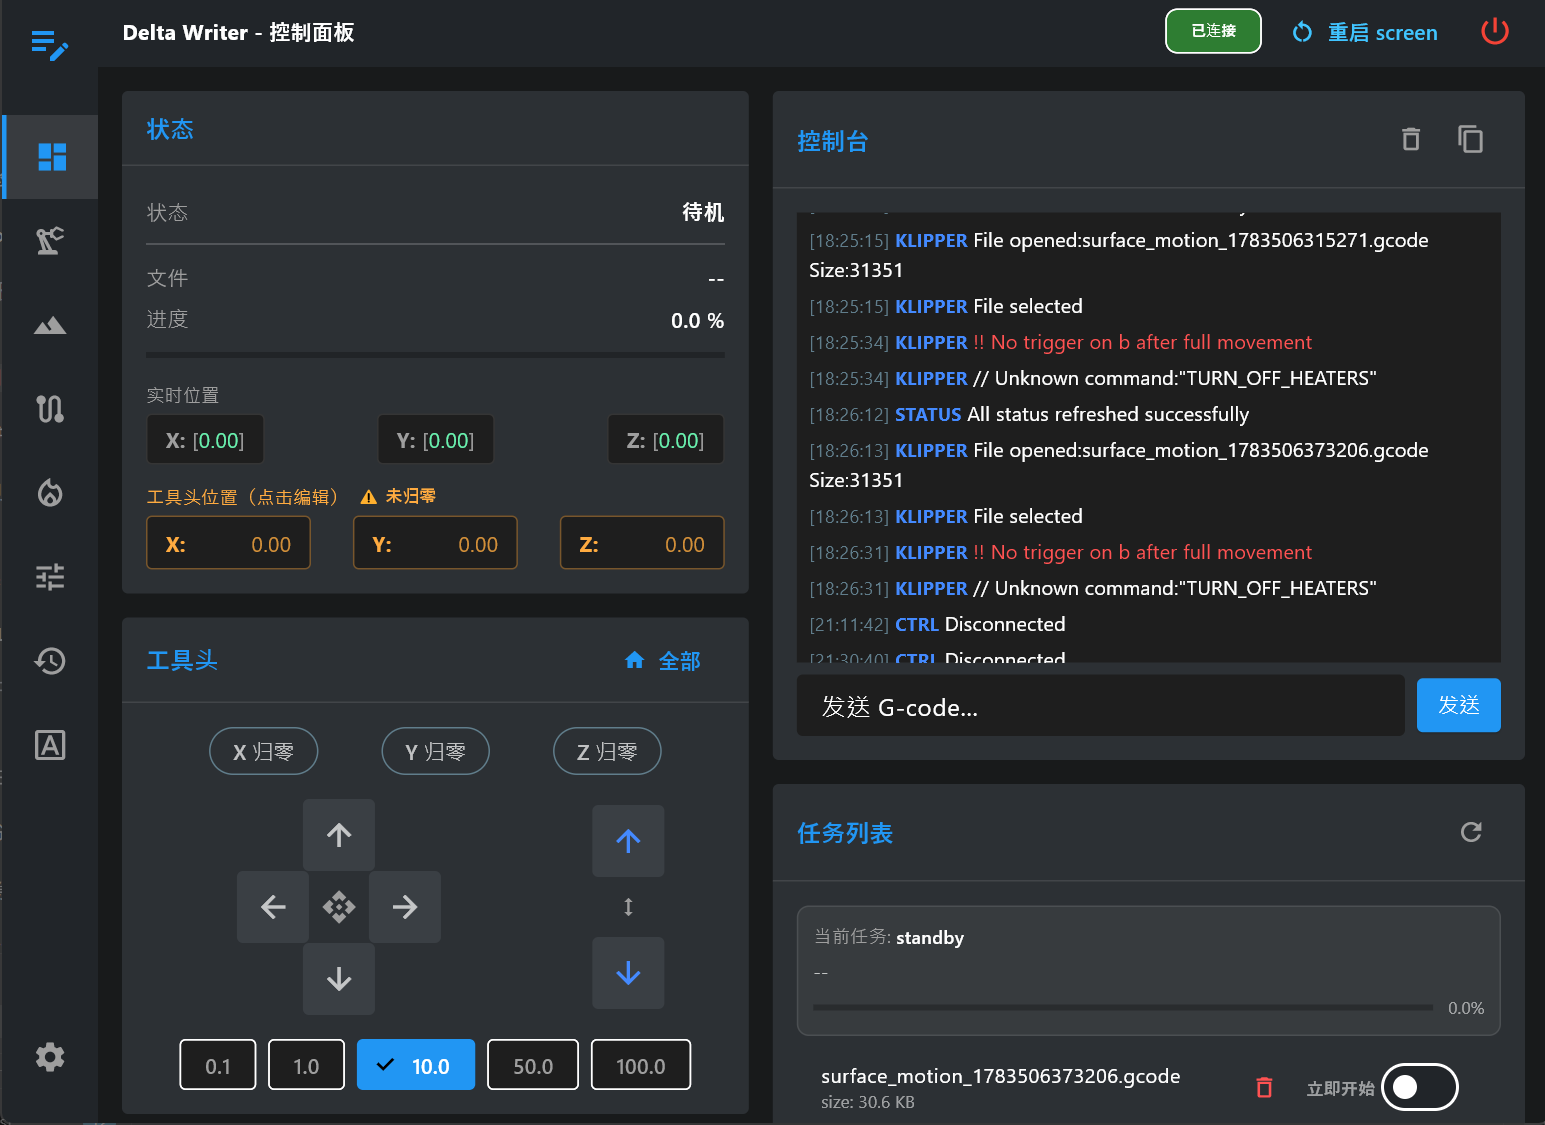
\includegraphics[width=0.6\textwidth,keepaspectratio]{assets/img/控制面板.png}
  \caption{控制主界面图}
  \label{fig:control_panel}
\end{figure}

\paragraph{参数校准模块}
参数校准模块面向视觉标定、机械坐标系对齐和误差补偿。界面以阶段卡片组织流程，包括床面 ChArUco 外参采集、机械坐标系对齐、误差采样网格、坐标系与末端偏移拟合以及可选的机构参数拟合。这一思路与平面标定板相机标定及视觉基准点检测方法一致\cite{zhang2000calibration,garrido2014aruco,olson2011apriltag}。

执行标定时，上位机控制器会先根据需要发送 \texttt{EMM\_HOME\_AND\_CLEAR}、\texttt{G90}、\texttt{G1} 和 \texttt{M400} 等指令，将机械臂移动到清晰拍摄位置或采样点。随后控制器以外部进程方式启动 Python 脚本，传入相机内参、标定板原点、主机地址、快照地址和输出目录等参数。脚本完成采图、角点检测、姿态估计和误差统计后生成 JSON 结果、叠加图和统计摘要，上位机再读取最新结果并刷新界面。
\begin{figure}[htbp]
  \centering
  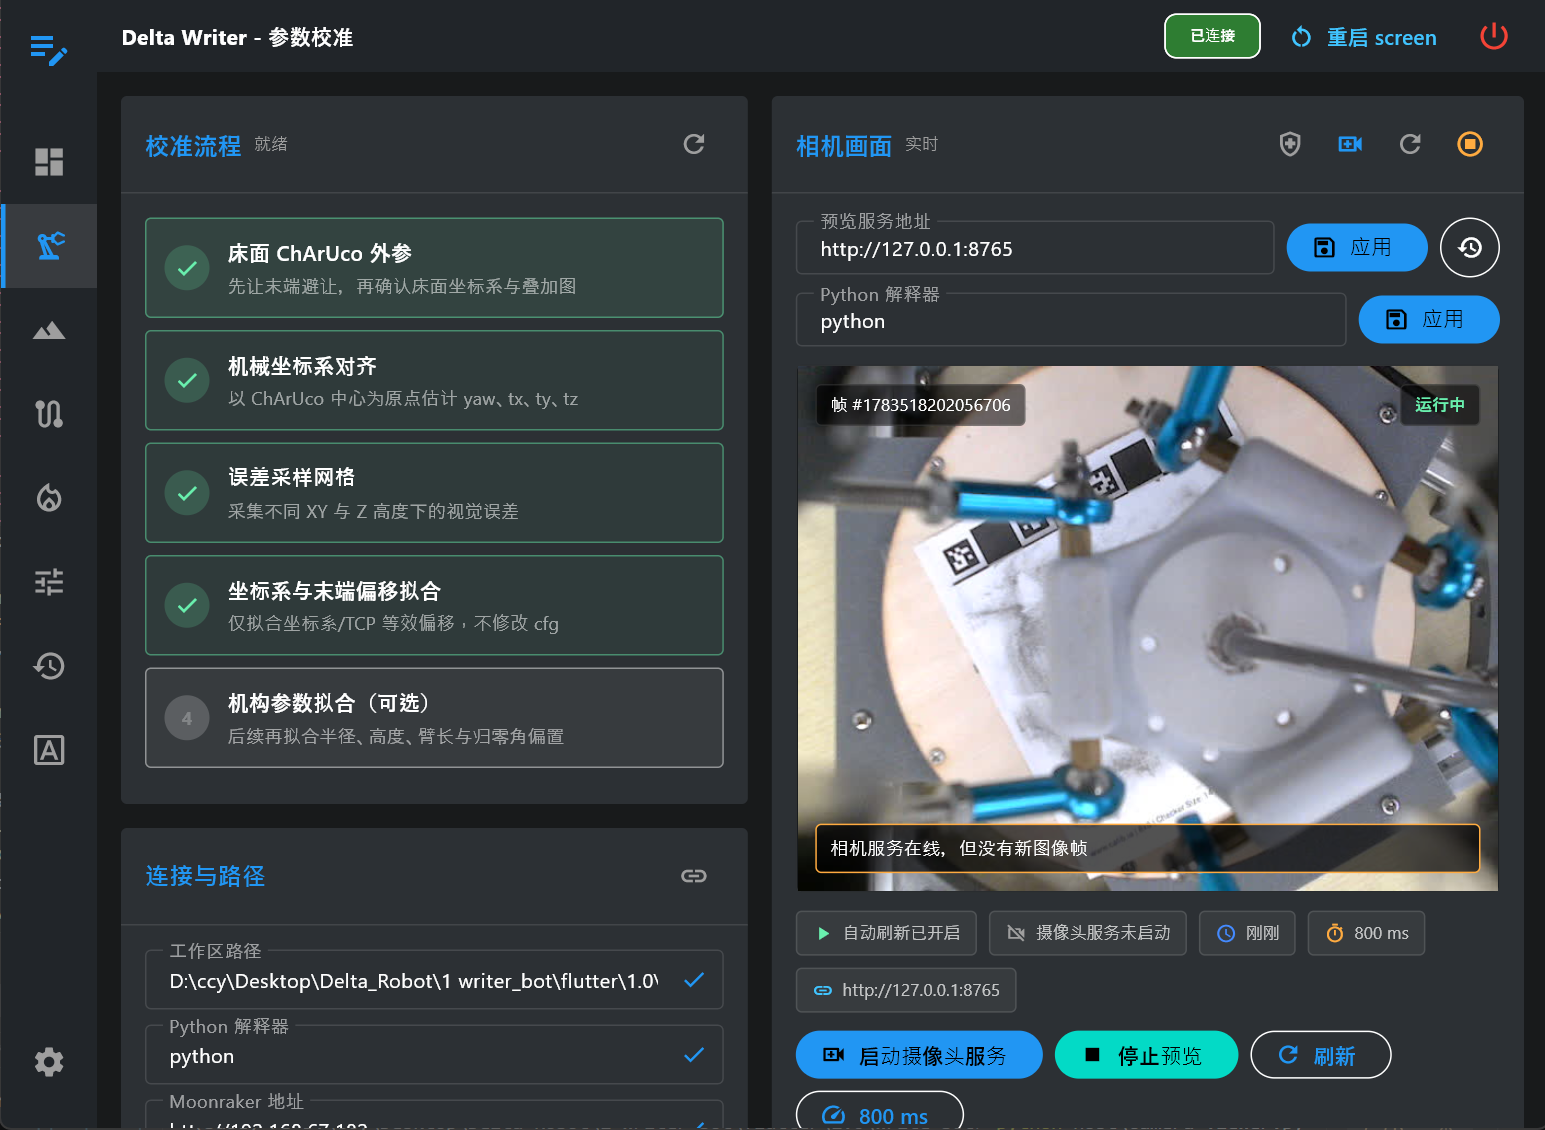
\includegraphics[width=0.6\textwidth,keepaspectratio]{assets/img/参数校准界面.png}
  \caption{参数校准界面图}
  \label{fig:param_panel}
\end{figure}

\paragraph{曲面模块}
曲面模块用于把二维文字、图案或 DXF 轨迹映射到三维曲面工件上。该模块支持 STL 模型导入、DXF 轨迹导入、曲面扫描点云读取、模型与点云配准、工件图像定位、曲面高度采样、轨迹生成、轨迹校准、G-code 导出和执行前验证。STL 解析器读取三角面片并计算模型包围盒，DXF 解析器支持直线、多段线、圆弧和圆等实体，并将其转换为可采样的二维折线轨迹。

模型配准过程首先根据用户选择的接触面建立初始对齐关系，然后从 STL 模型和扫描点云中采样点集。配准服务通过初始偏航搜索和最近邻匹配估计刚体变换，在迭代过程中不断更新旋转和平移参数，直到均方根误差低于阈值或达到最大迭代次数。配准结果包含初始误差、最终误差、匹配点数、迭代次数、是否收敛以及模型和点云边界诊断信息，用于判断扫描数据与模型是否可靠对齐。

轨迹生成阶段以上位机中的二维路径为输入，按照设定采样步长在 STL 表面查询高度，并结合床面 Z 值、离面间隙和视觉标定结果计算机器坐标。对于曲面局部坐标到机械坐标的转换，上位机会生成中间 JSON 文件并调用坐标转换脚本，得到每个采样点对应的机器 X、Y、Z 坐标。曲面表面采样和恒距路径生成与自由曲面覆盖路径规划的核心思路一致\cite{atkar2005coverage}。生成 G-code 时，程序会写入单位和绝对坐标指令，并按顺序输出各采样点的 \texttt{G1} 运动命令，末尾等待运动完成并自动回零。执行前，验证流程可抽取关键点移动并采集相机图像，通过检测脚本确认轨迹与工件位置是否一致。
\begin{figure}[htbp]
  \centering
  \begin{minipage}[t]{0.48\textwidth}
    \centering
    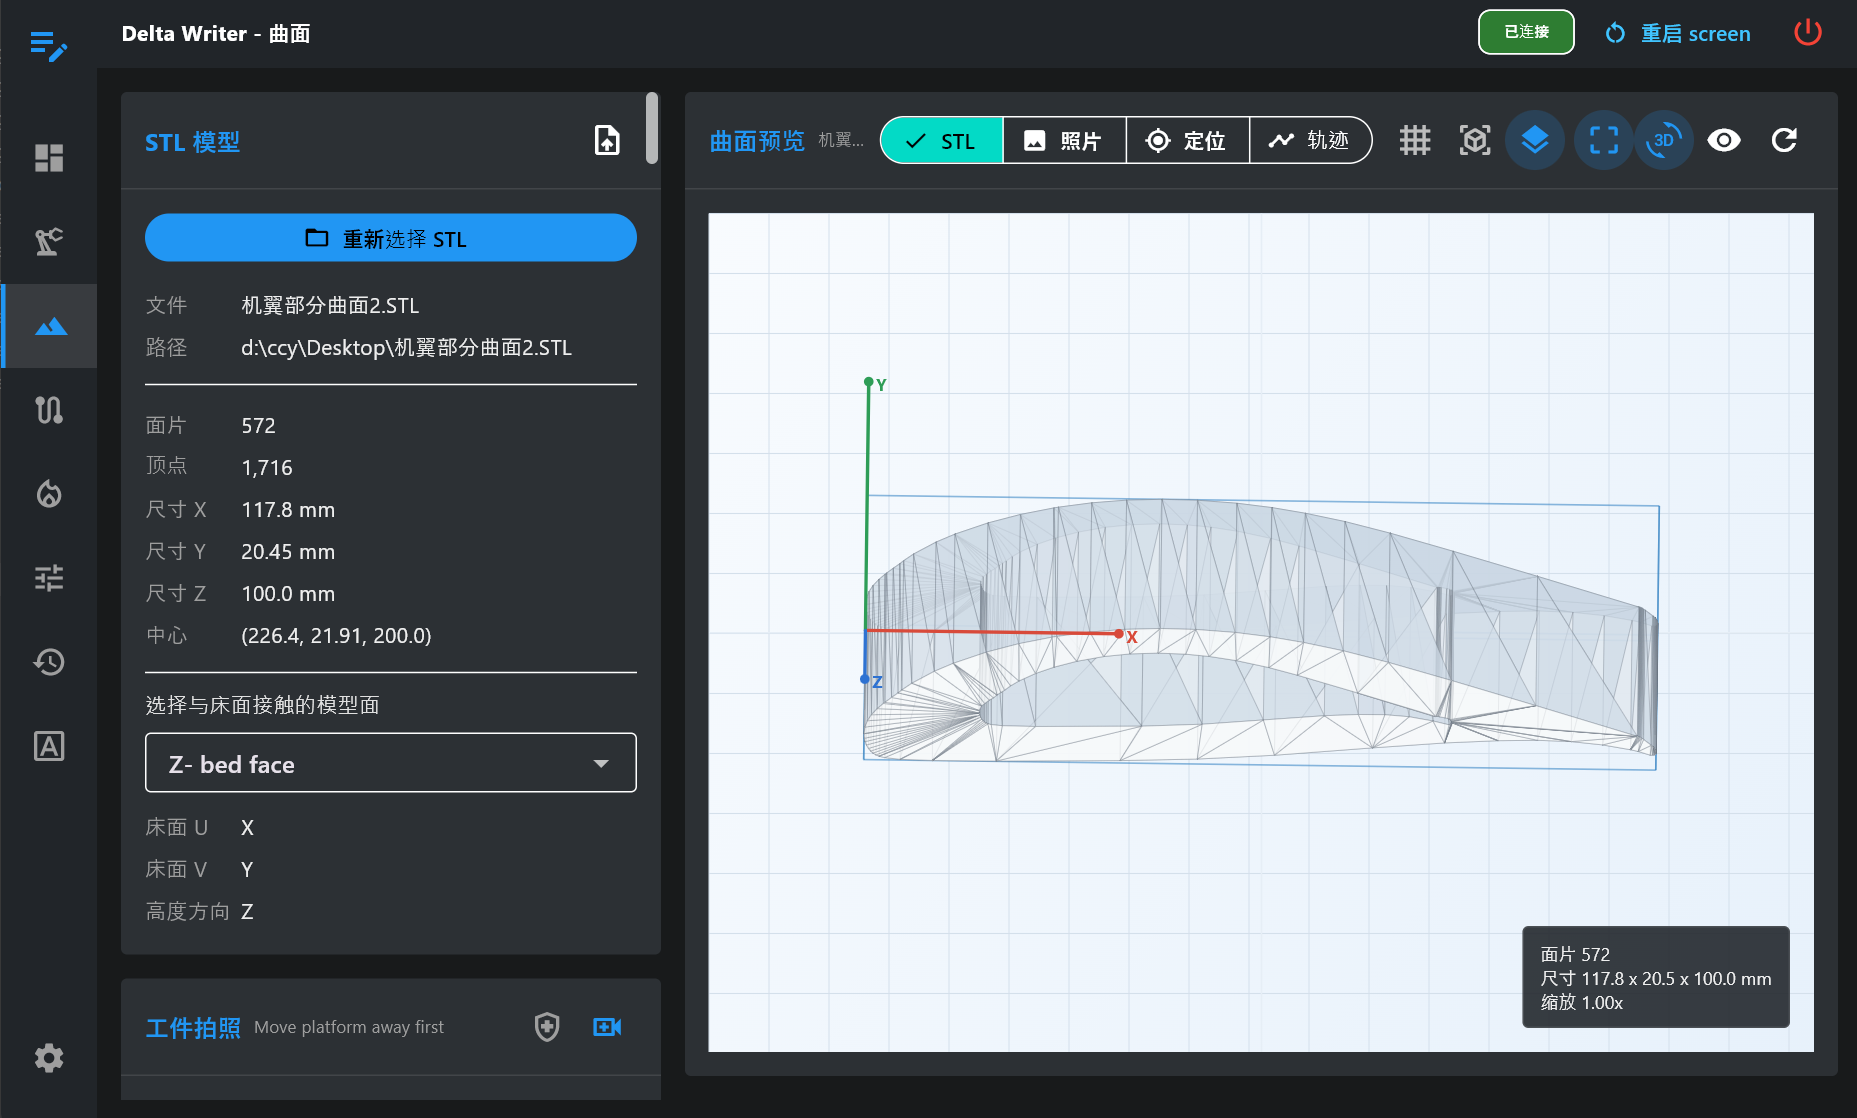
\includegraphics[width=\linewidth,keepaspectratio]{assets/img/曲面界面.png}
    \caption{曲面模块界面图}
    \label{fig:curve_panel}
  \end{minipage}
  \hfill
  \begin{minipage}[t]{0.48\textwidth}
    \centering
    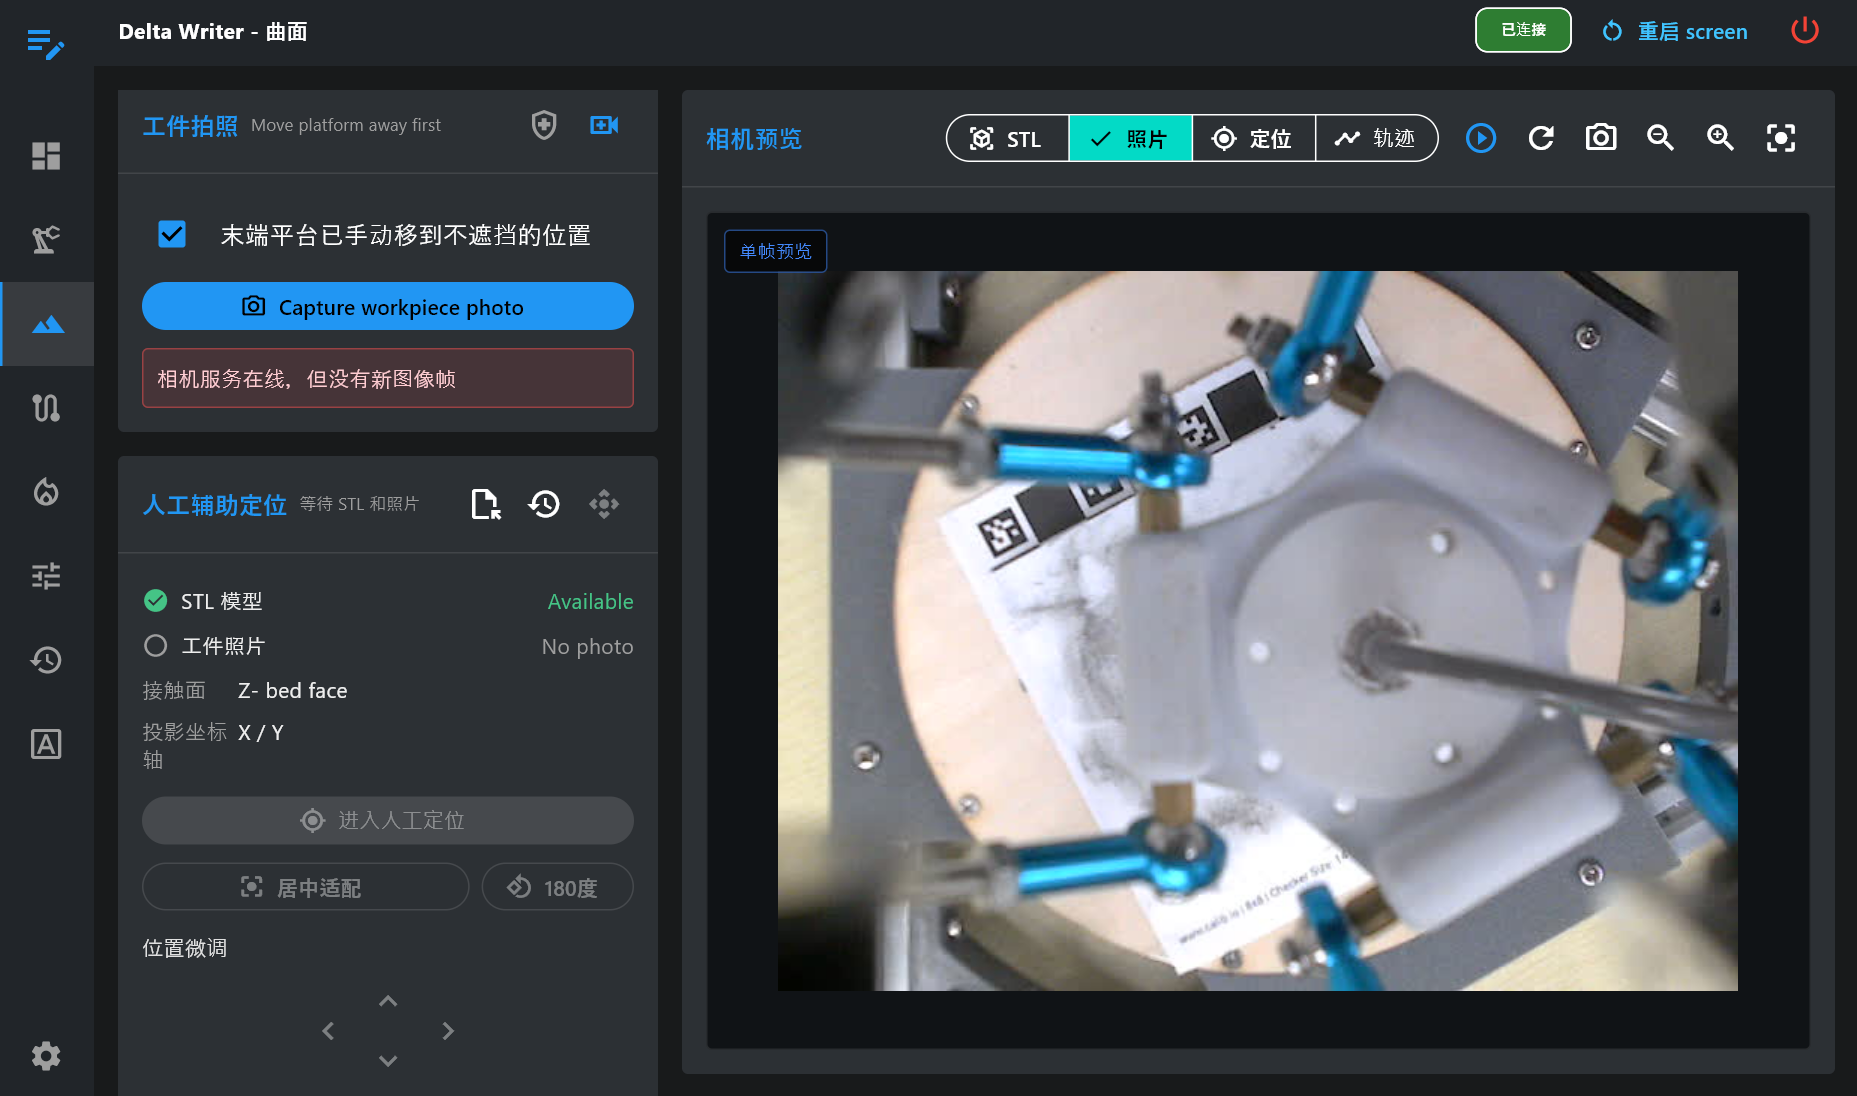
\includegraphics[width=\linewidth,keepaspectratio]{assets/img/拍照界面.png}
    \caption{拍照界面图}
    \label{fig:photo_panel}
  \end{minipage}

  \vspace{1em}

  \begin{minipage}[t]{0.48\textwidth}
    \centering
    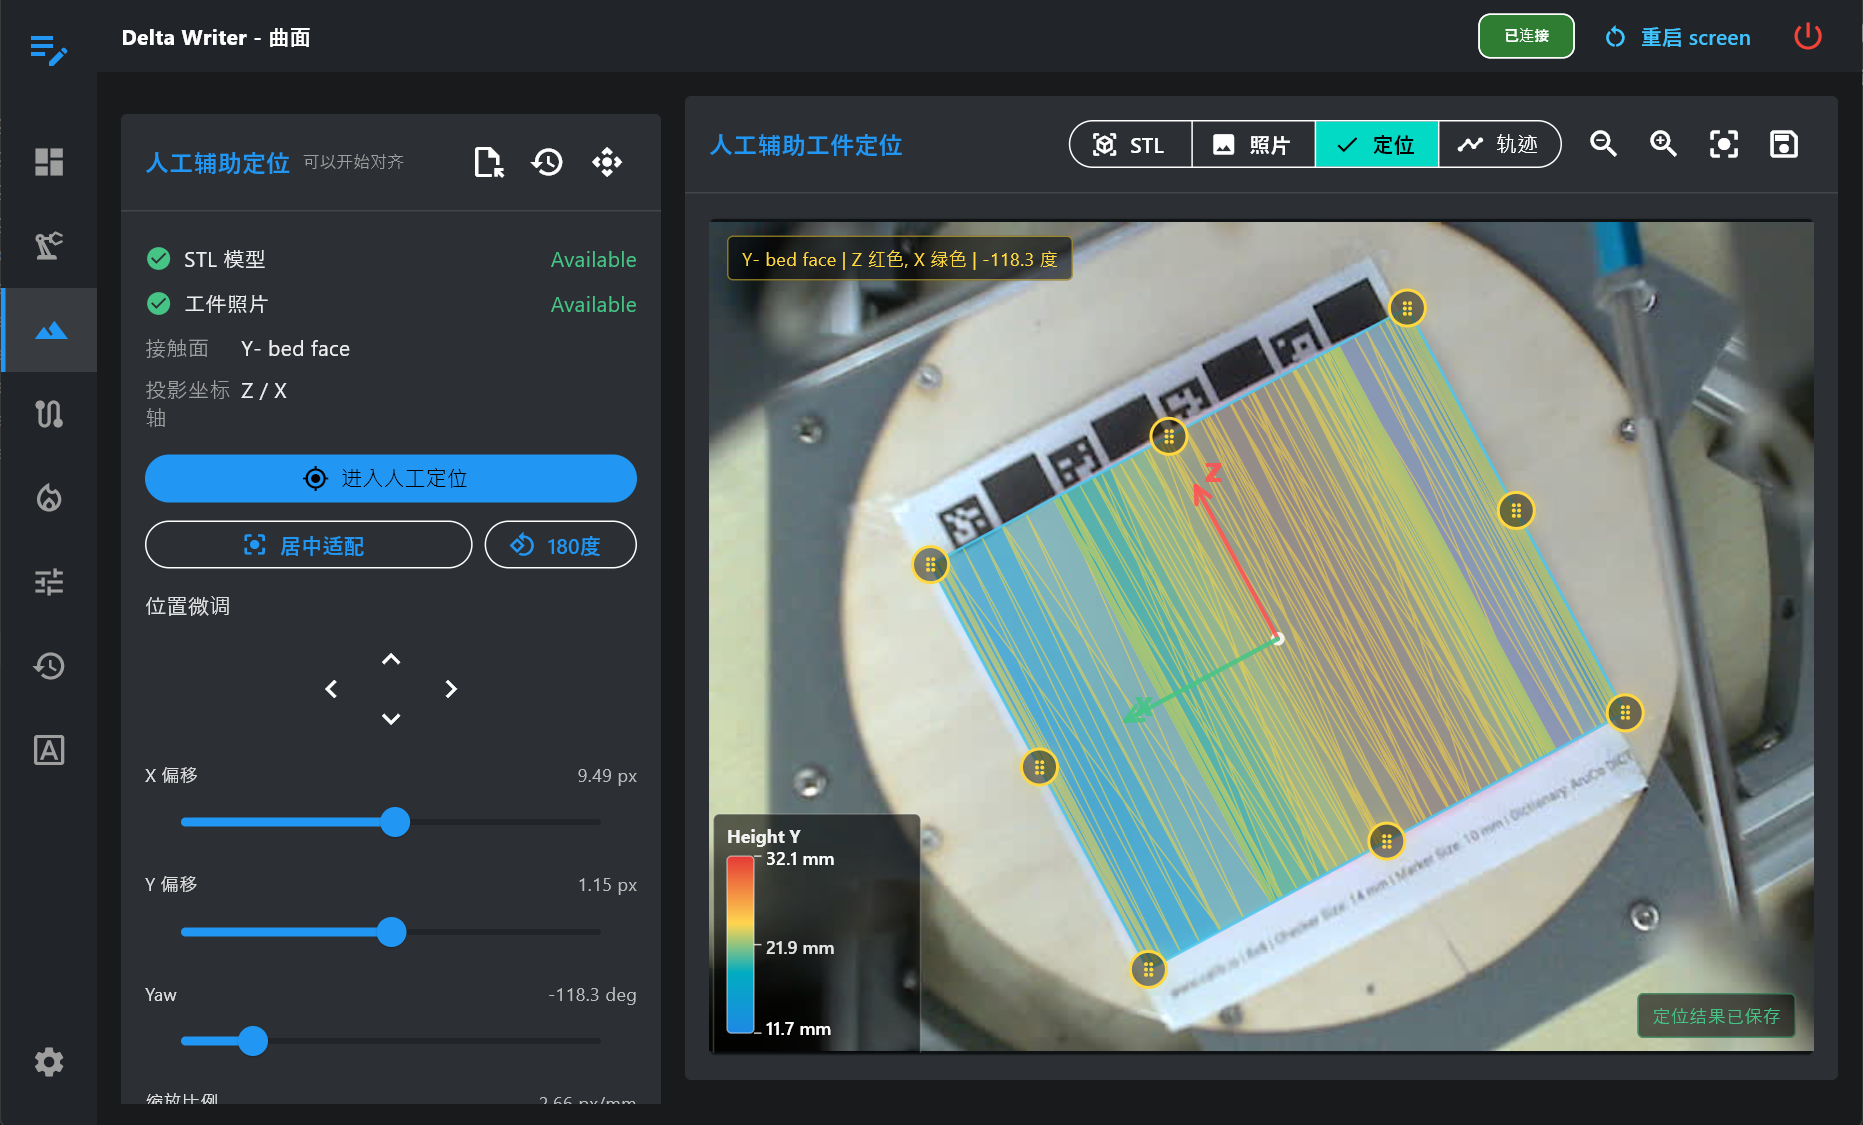
\includegraphics[width=\linewidth,keepaspectratio]{assets/img/校准界面.png}
    \caption{校准界面图}
    \label{fig:calibration_panel}
  \end{minipage}
  \hfill
  \begin{minipage}[t]{0.48\textwidth}
    \centering
    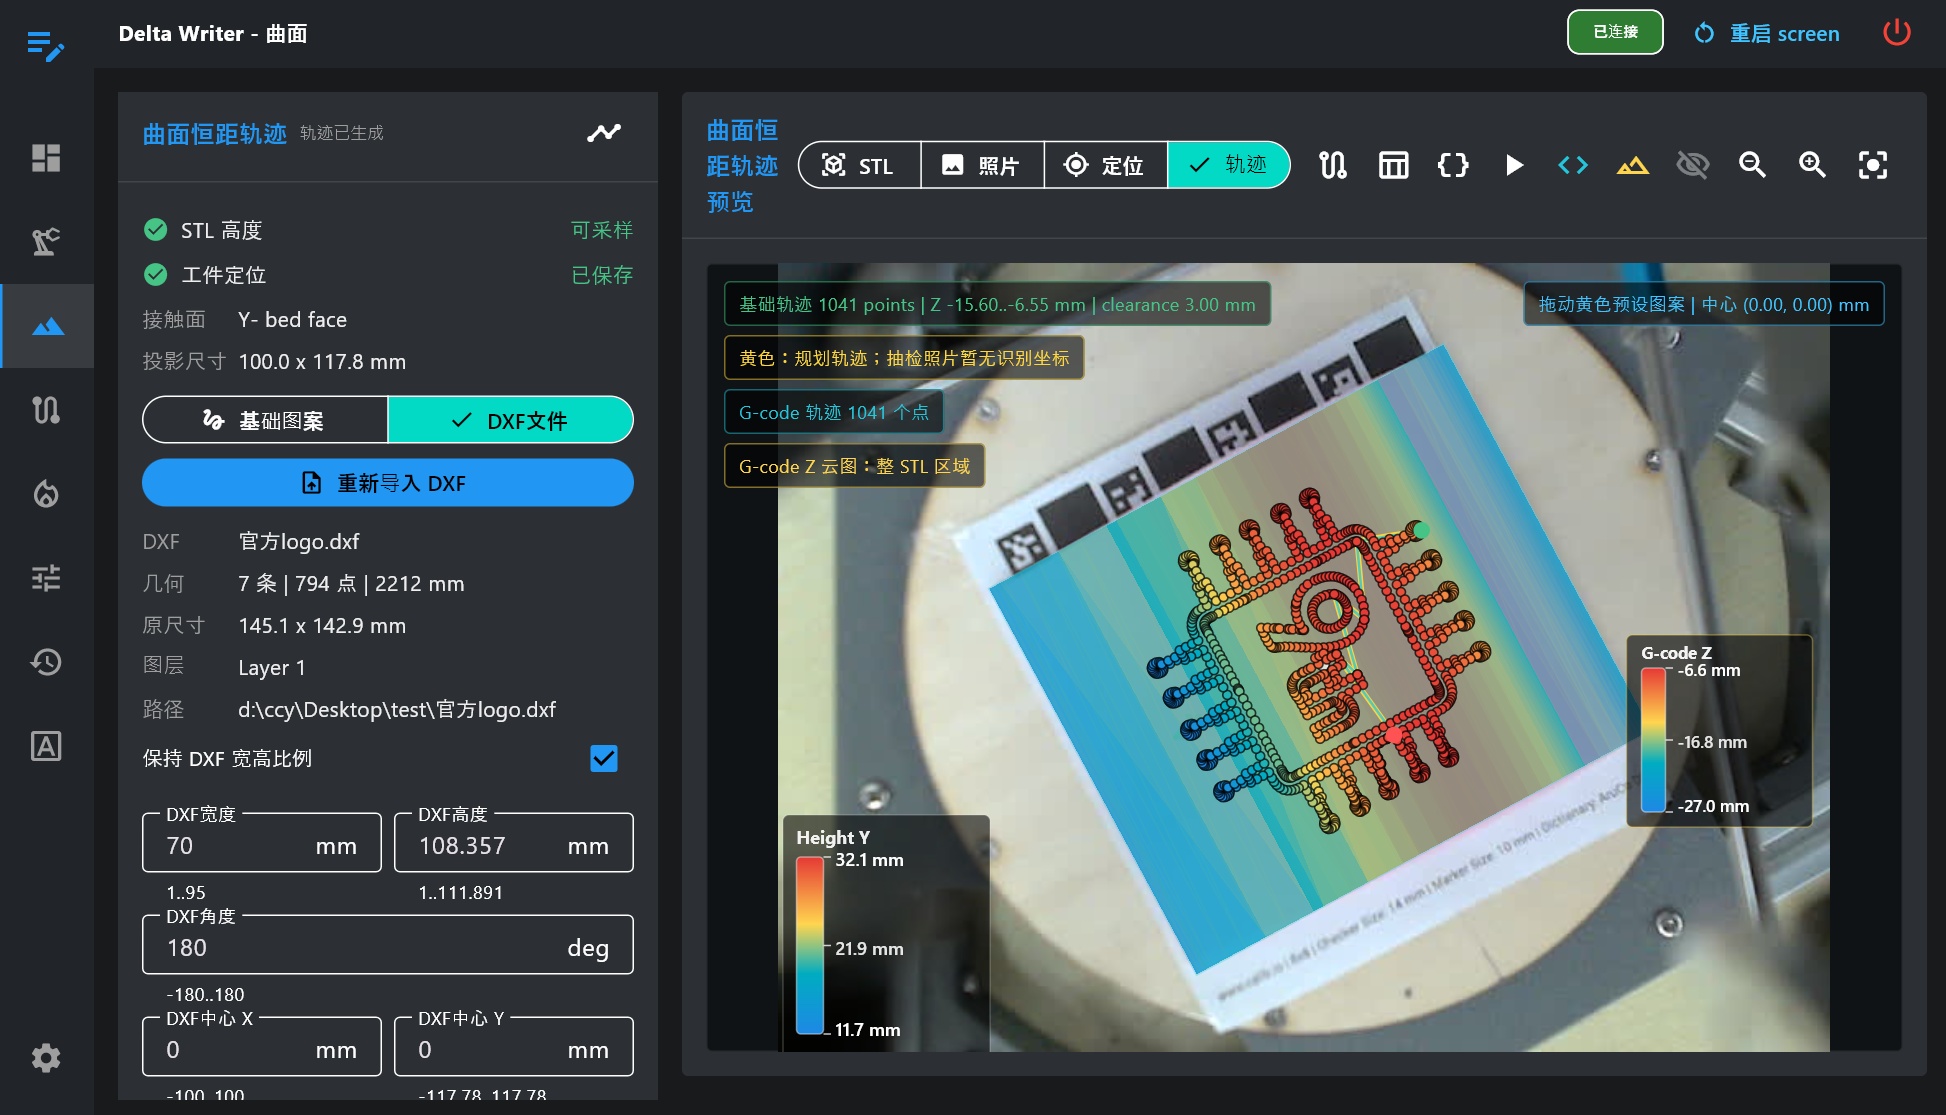
\includegraphics[width=\linewidth,keepaspectratio]{assets/img/轨迹界面.png}
    \caption{轨迹界面图}
    \label{fig:trajectory_panel}
  \end{minipage}
\end{figure}

\paragraph{激光加工模块}
激光页面将书写和雕刻两类任务统一在同一条 G-code 生成链路下。书写模式根据纸张尺寸、网格规格、用户字体或标准字体生成文字路径；雕刻模式可从 DXF 文件或位图图像生成路径，DXF 路径由几何实体解析得到，位图路径则通过阈值化和逐行扫描把深色像素区域转换为连续线段。用户可设置激光功率、加工速度、图案尺寸、镜像、旋转、偏移、起始点和视觉补偿等参数。

\begin{figure}[htbp]
  \centering
  \begin{minipage}[t]{0.48\textwidth}
    \centering
    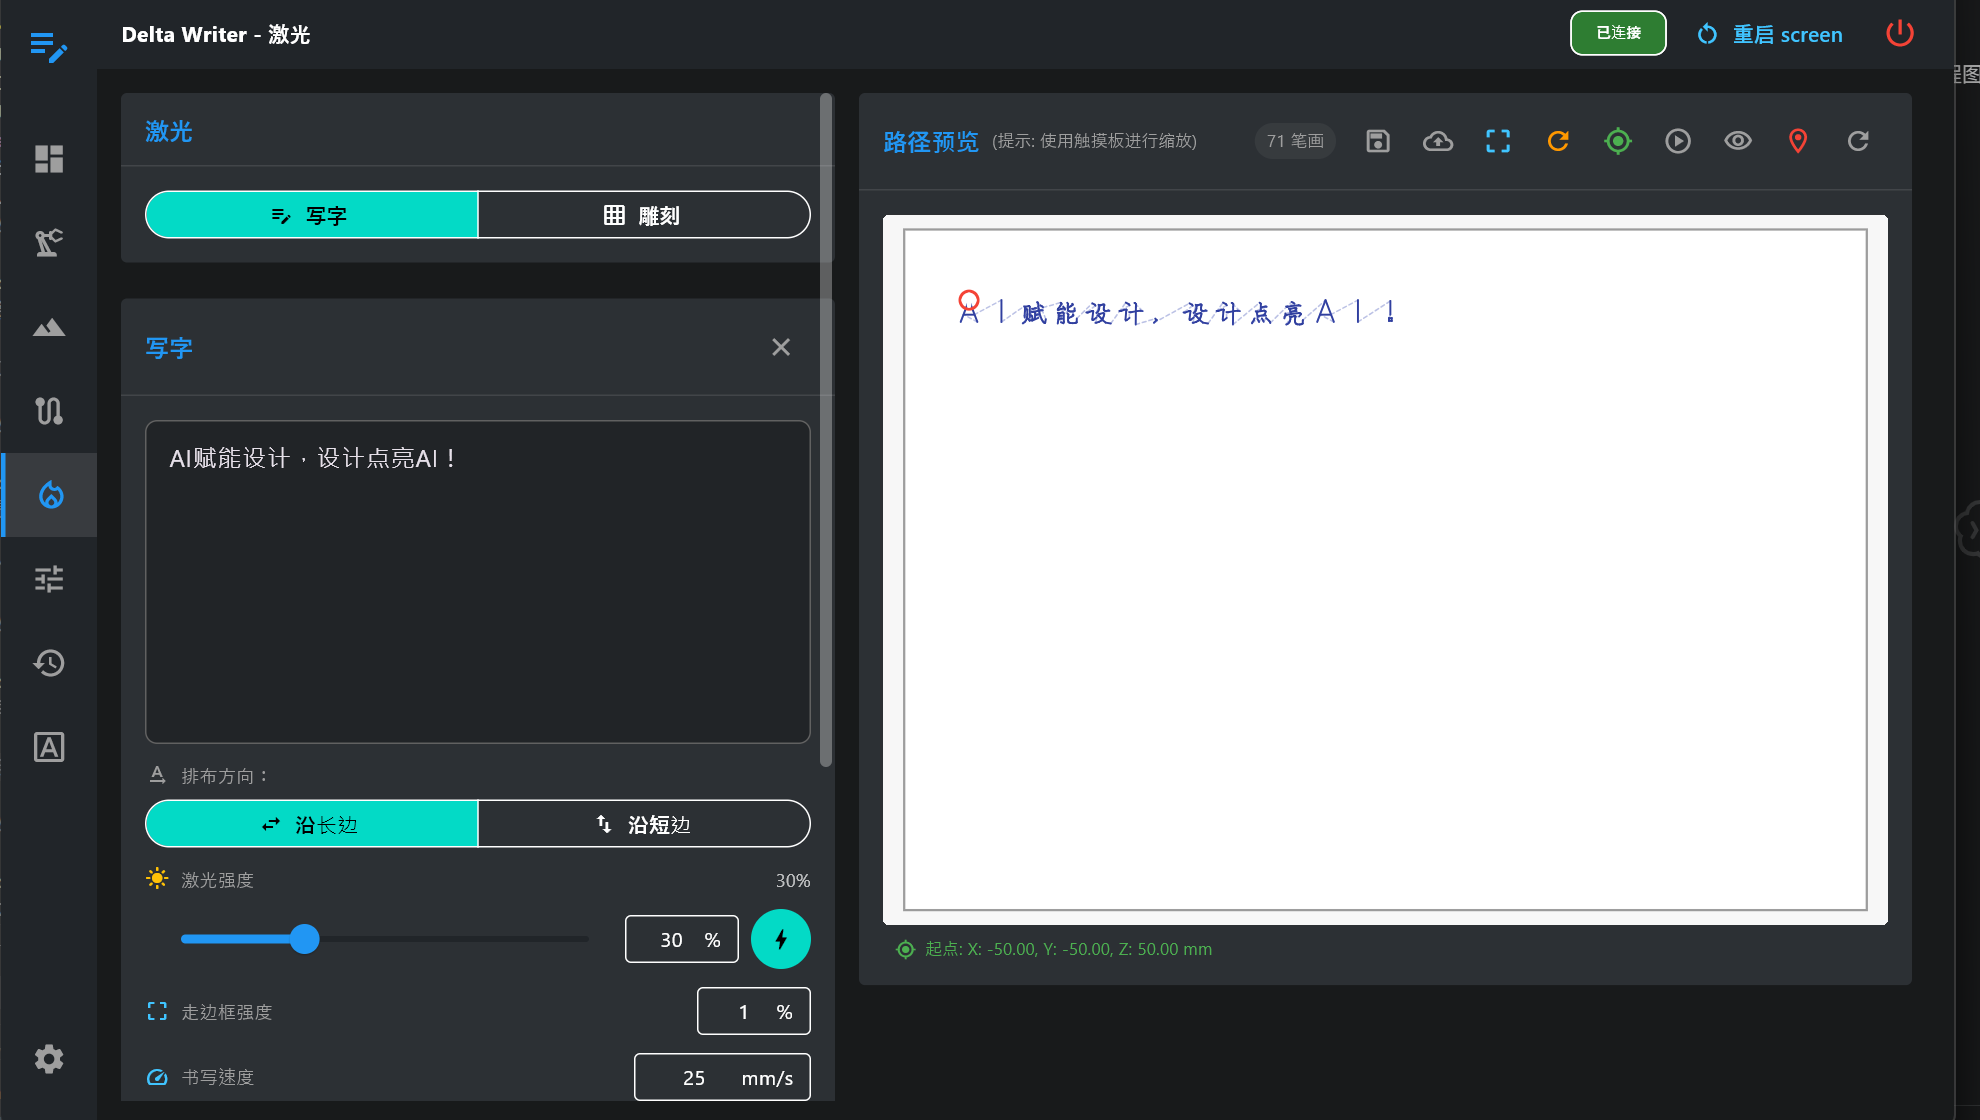
\includegraphics[width=\linewidth,keepaspectratio]{assets/img/激光书写界面.png}
    \caption{激光书写界面图}
    \label{fig:write_panel}
  \end{minipage}
  \hfill
  \begin{minipage}[t]{0.48\textwidth}
    \centering
    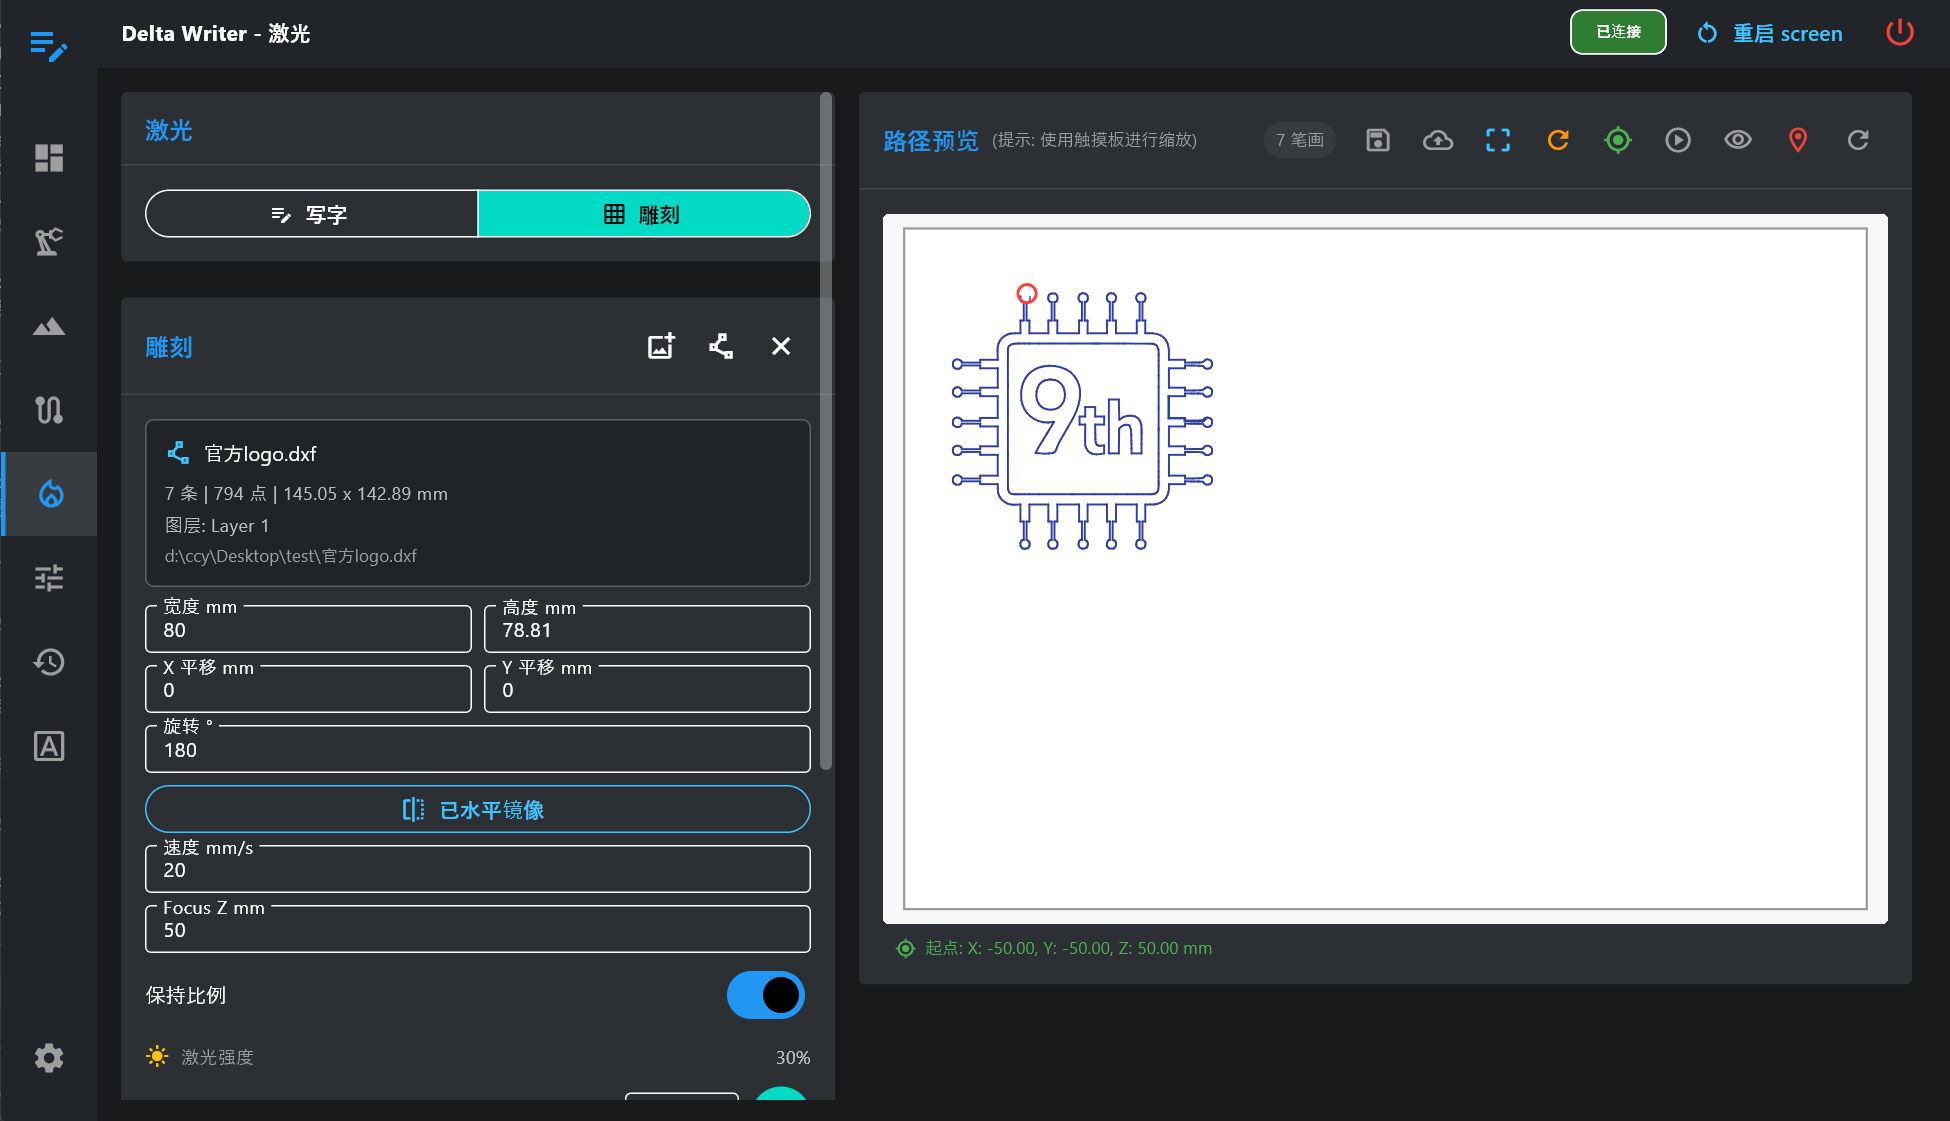
\includegraphics[width=\linewidth,keepaspectratio]{assets/img/激光雕刻界面.png}
    \caption{激光雕刻界面图}
    \label{fig:laser_panel}
  \end{minipage}
\end{figure}




\paragraph{本机触控屏显示模块}
本机触控屏显示程序作为 PC 上位机之外的现场操作入口，运行在机器人主机本地。程序启动后会读取屏幕配置、加载主题和页面面板，建立 REST 客户端与 WebSocket 客户端，并订阅坐标、任务状态、输出引脚、温度、文件进度等对象。屏幕界面根据订阅数据切换就绪、运行中、暂停、错误、断开连接等状态，并可调用主机接口发送 G-code、启动或暂停任务、取消任务以及重启相关服务。


\begin{figure}[htbp]
  \centering
  \begin{minipage}[t]{0.48\textwidth}
    \centering
    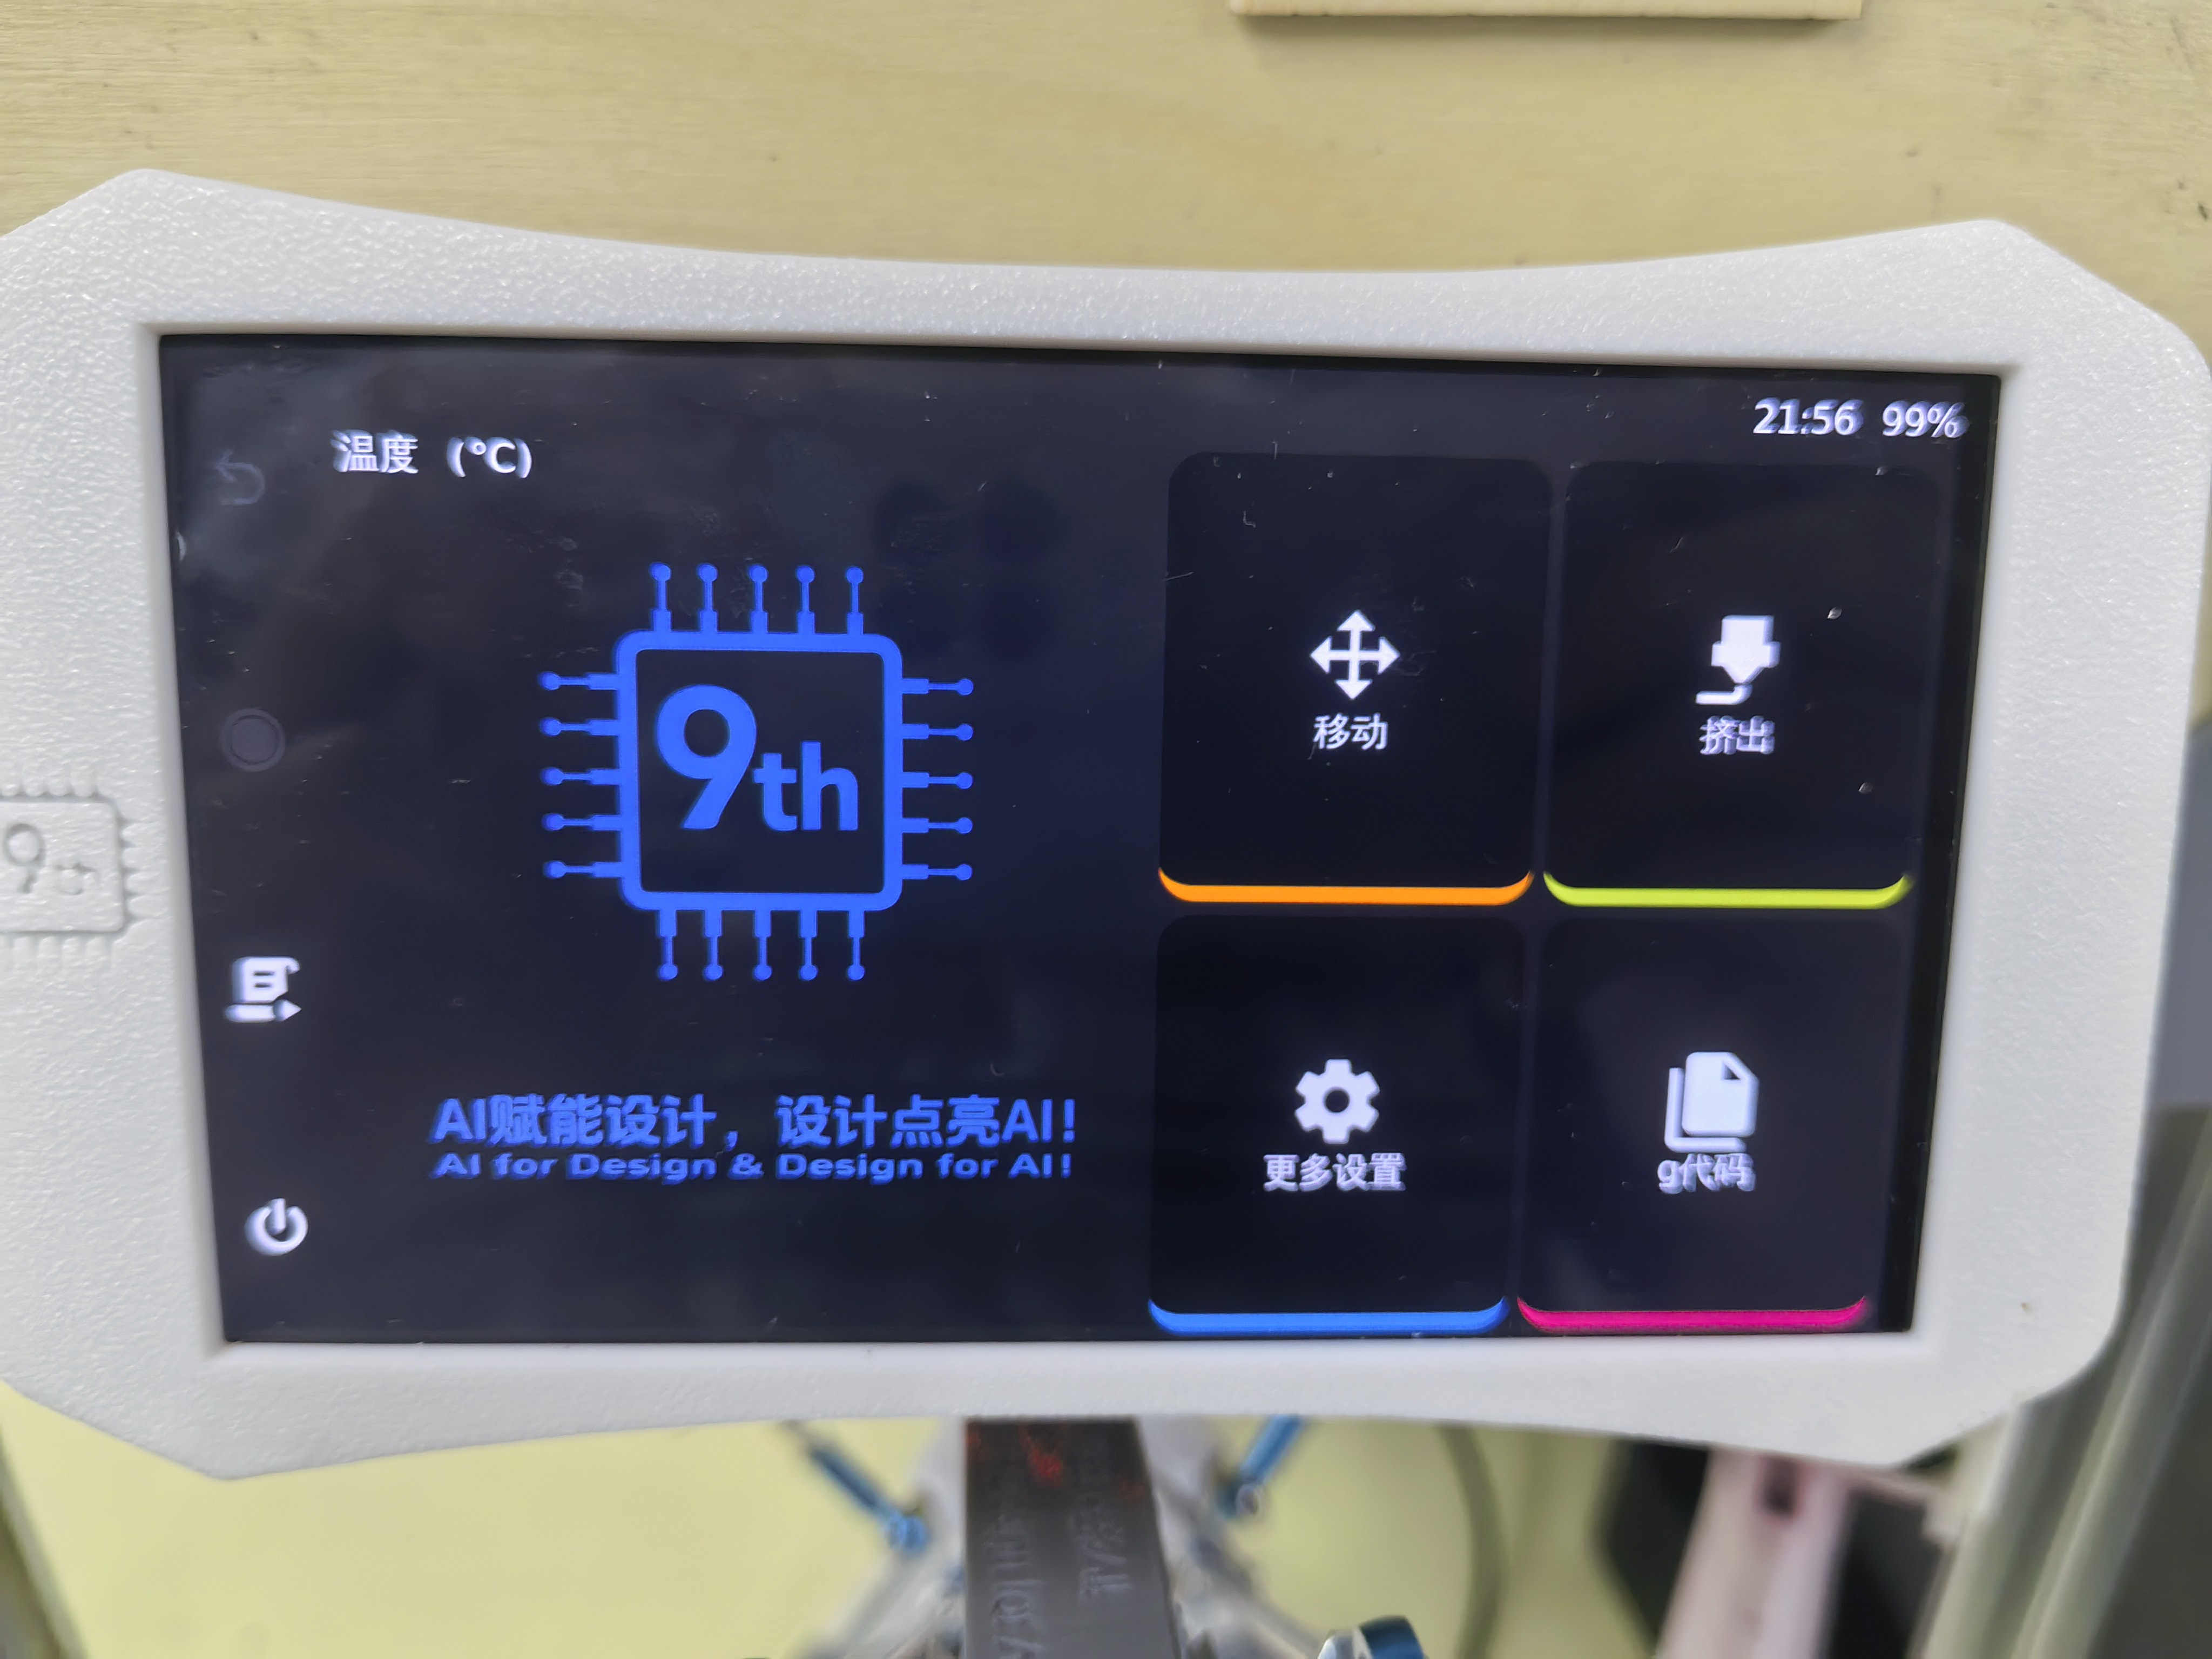
\includegraphics[width=\linewidth,keepaspectratio]{assets/img/主界面.jpg}
    \caption{触摸屏主界面图}
    \label{fig:main_panel}
  \end{minipage}
  \hfill
  \begin{minipage}[t]{0.48\textwidth}
    \centering
    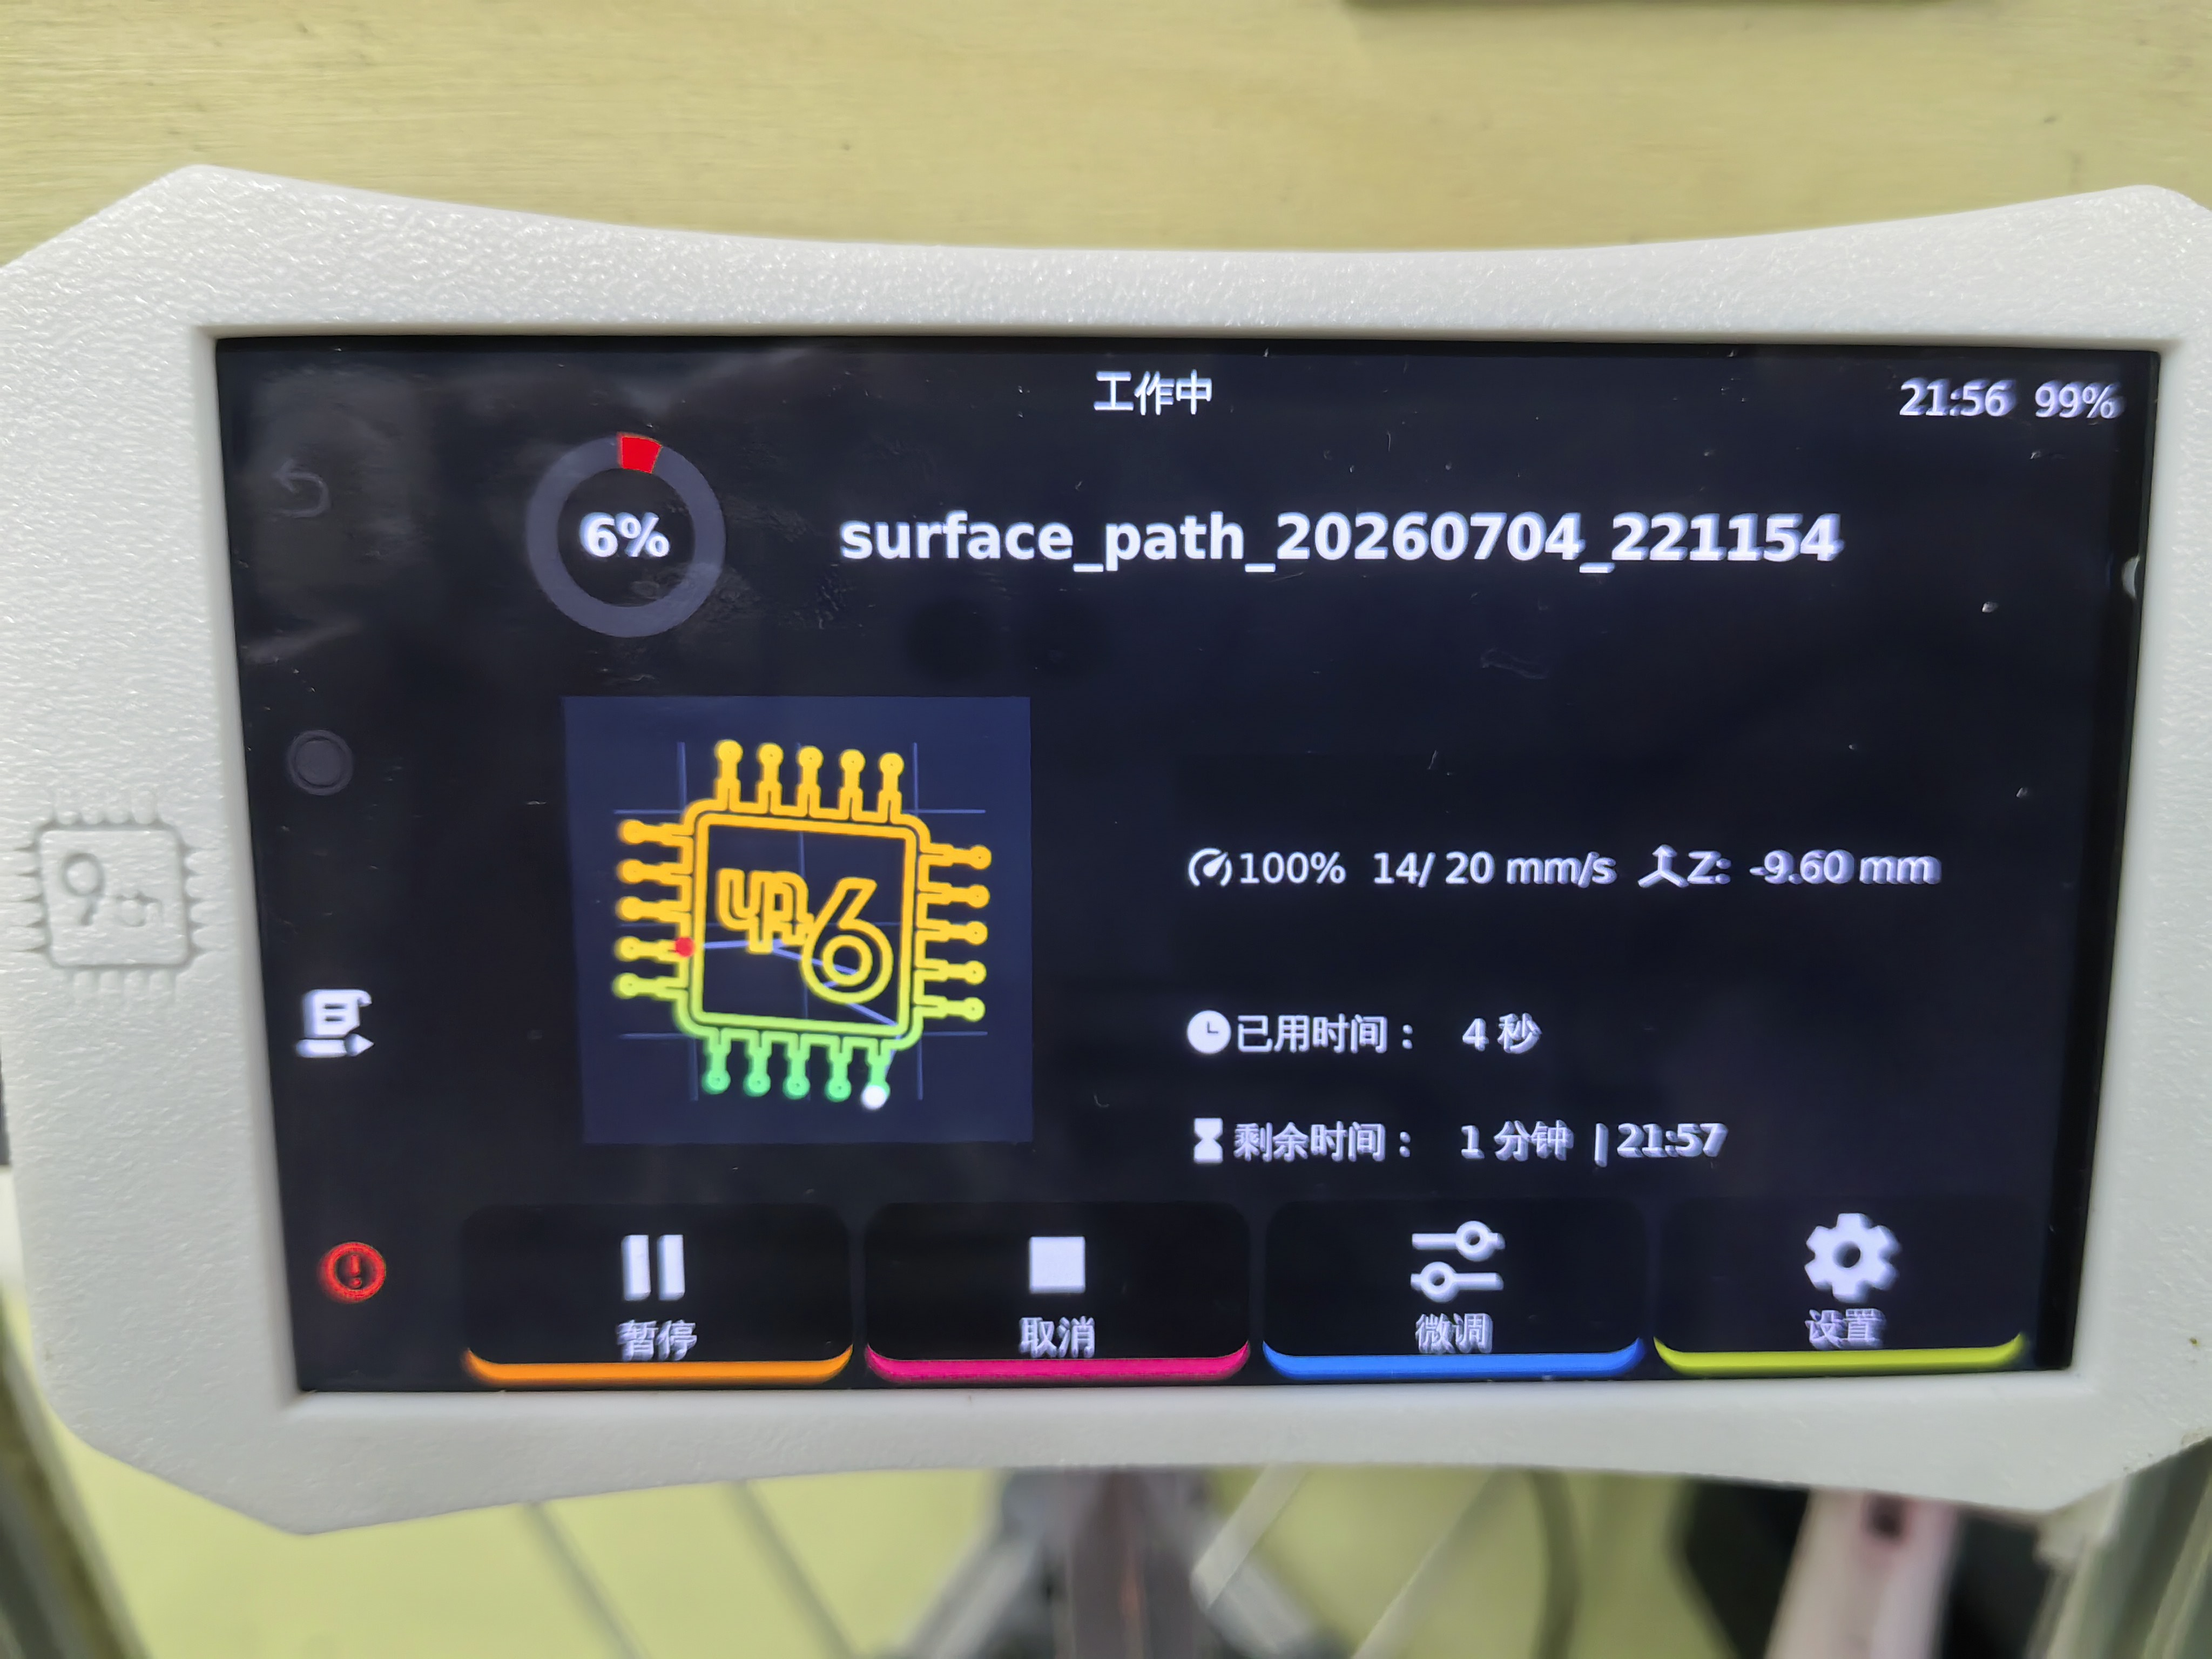
\includegraphics[width=\linewidth,keepaspectratio]{assets/img/运行界面.jpg}
    \caption{运行界面图}
    \label{fig:running_panel}
  \end{minipage}
\end{figure}

\paragraph{STM32F407 实时控制模块}
STM32F407 固件由启动初始化、命令通信、任务调度、步进输出、GPIO/PWM 输出和电机串口扩展几部分组成。系统上电后，启动函数完成复位检查、时钟和外设基础配置，然后进入调度主循环。命令通信模块负责解析主机发来的二进制命令、校验帧数据、提取命令参数，并通过响应帧把执行结果返回主机。任务调度模块维护定时器队列和周期任务，在等待事件和执行任务之间循环切换，为步进脉冲和外设动作提供统一的时间基准。

步进输出模块在配置阶段绑定每个电机的 step、dir 和 enable 引脚，在运动阶段按照队列中的步数、间隔和方向参数触发定时事件。每次事件到达时，固件设置或复位 step 引脚，并根据剩余步数和加减速参数安排下一次事件，从而形成稳定的脉冲序列。GPIO/PWM 输出模块负责普通数字输出和 PWM 输出，本项目中的激光控制即由主机侧的 \texttt{SET\_PIN} 指令映射到底层 PWM 引脚，固件按照配置的周期和占空比更新输出。

针对闭环步进驱动器，固件增加了 USART2 串口通信模块，其主机扩展、MCU 命令和驱动器响应关系如图~\ref{fig:emm_usart_sequence} 所示。主机侧将 \texttt{EMM} 系列宏封装为串口配置和数据传输命令；STM32F407 固件在 PA2、PA3 上完成字节发送、超时接收和响应回传，从而支持清零、使能、读取位置、回零、记录轨迹点和播放轨迹点等高层动作。

\begin{figure}[htbp]
  \centering
  \resizebox{\textwidth}{!}{%
  \begin{tikzpicture}[
    font=\footnotesize,
    >=Stealth,
    actor/.style={draw, rounded corners=1.5mm, align=center, minimum width=23mm, minimum height=8mm, inner sep=2pt, fill=#1},
    actor/.default=blue!8,
    lifeline/.style={densely dashed, gray!65},
    msg/.style={->, thick},
    ret/.style={->, dashed, thick, gray!75},
    lab/.style={font=\scriptsize, align=center, fill=white, text=black, inner sep=1pt},
    bandlabel/.style={font=\scriptsize\bfseries, anchor=west, align=left}
  ]
    \begin{scope}[on background layer]
      \filldraw[fill=cyan!6, draw=cyan!35, rounded corners=1mm] (-1.70,-0.55) rectangle (13.15,-2.35);
      \filldraw[fill=purple!6, draw=purple!35, rounded corners=1mm] (-1.70,-2.70) rectangle (13.15,-5.80);
    \end{scope}

    \node[actor=blue!10] (host) at (0,0) {固件\\EMM 扩展};
    \node[actor=green!10] (queue) at (3,0) {MCU\\命令队列};
    \node[actor=orange!12] (firmware) at (6,0) {STM32F407\\固件};
    \node[actor=cyan!10] (usart) at (9,0) {USART2\\PA2/PA3};
    \node[actor=red!10] (driver) at (12,0) {闭环步进\\驱动器};

    \foreach \x in {0,3,6,9,12} {
      \draw[lifeline] (\x,-0.45) -- (\x,-6.05);
    }

    \node[bandlabel] at (-1.60,-0.82) {初始化};
    \draw[msg] (0,-1.12) -- node[lab, above] {读取配置：波特率、ID、超时} (3,-1.12);
    \draw[msg] (3,-1.42) -- node[lab, above] {\texttt{config\_emm\_usart}} (6,-1.42);
    \draw[msg] (6,-1.72) -- node[lab, above] {配置串口参数} (9,-1.72);
    \draw[ret] (6,-2.02) -- node[lab, above] {OID 就绪} (0,-2.02);

    \node[bandlabel] at (-1.60,-2.97) {一次驱动器读写};
    \draw[msg] (0,-3.28) -- node[lab, above] {\texttt{EMM} 宏命令} (3,-3.28);
    \draw[msg] (3,-3.58) -- node[lab, above] {\texttt{emm\_usart\_transfer(write, read\_len)}} (6,-3.58);
    \draw[msg] (6,-3.88) -- node[lab, above] {清空接收区，等待 TXE/TC} (9,-3.88);
    \draw[msg] (9,-4.18) -- node[lab, above] {ID + 命令 + 校验帧} (12,-4.18);
    \draw[ret] (12,-4.58) -- node[lab, above] {位置/状态响应帧} (9,-4.58);
    \draw[ret] (9,-4.88) -- node[lab, above] {RXNE 或超时读取} (6,-4.88);
    \draw[ret] (6,-5.18) -- node[lab, above] {\texttt{emm\_usart\_response}} (3,-5.18);
    \draw[ret] (3,-5.48) -- node[lab, above] {更新状态与回调结果} (0,-5.48);
  \end{tikzpicture}%
  }
  \caption{闭环步进电机 USART2 通信时序图}
  \label{fig:emm_usart_sequence}
\end{figure}

该实时控制模块的关键输入包括主机下发的配置命令、运动队列、PWM 输出值和电机串口数据包；关键输出包括步进脉冲、方向信号、激光 PWM 信号、驱动器串口指令以及返回主机的状态响应。由于脉冲和 PWM 生成均在控制板本地完成，网络延迟和上位机负载不会直接影响实时运动时序，从而保证了 Delta 书写机器人在高速运动和激光加工过程中的稳定性。


\partheading{第三部分}{完成情况及性能参数}


\subsection{整体介绍}
系统整体实物如图~\ref{fig:system_front} 和图~\ref{fig:45} 所示。整机采用 Delta 并联机构，基座上固定三组步进电机及传动机构，三条运动支链连接至末端动平台；单目摄像头模块用于工件图像采集；电气控制盒内集成 STM32F407 控制板、闭环步进驱动器及电源模块，顶部配有主机触控屏用于人机交互和现场调试。
\begin{figure}[htbp]
  \centering
  \begin{minipage}[t]{0.48\textwidth}
    \centering
    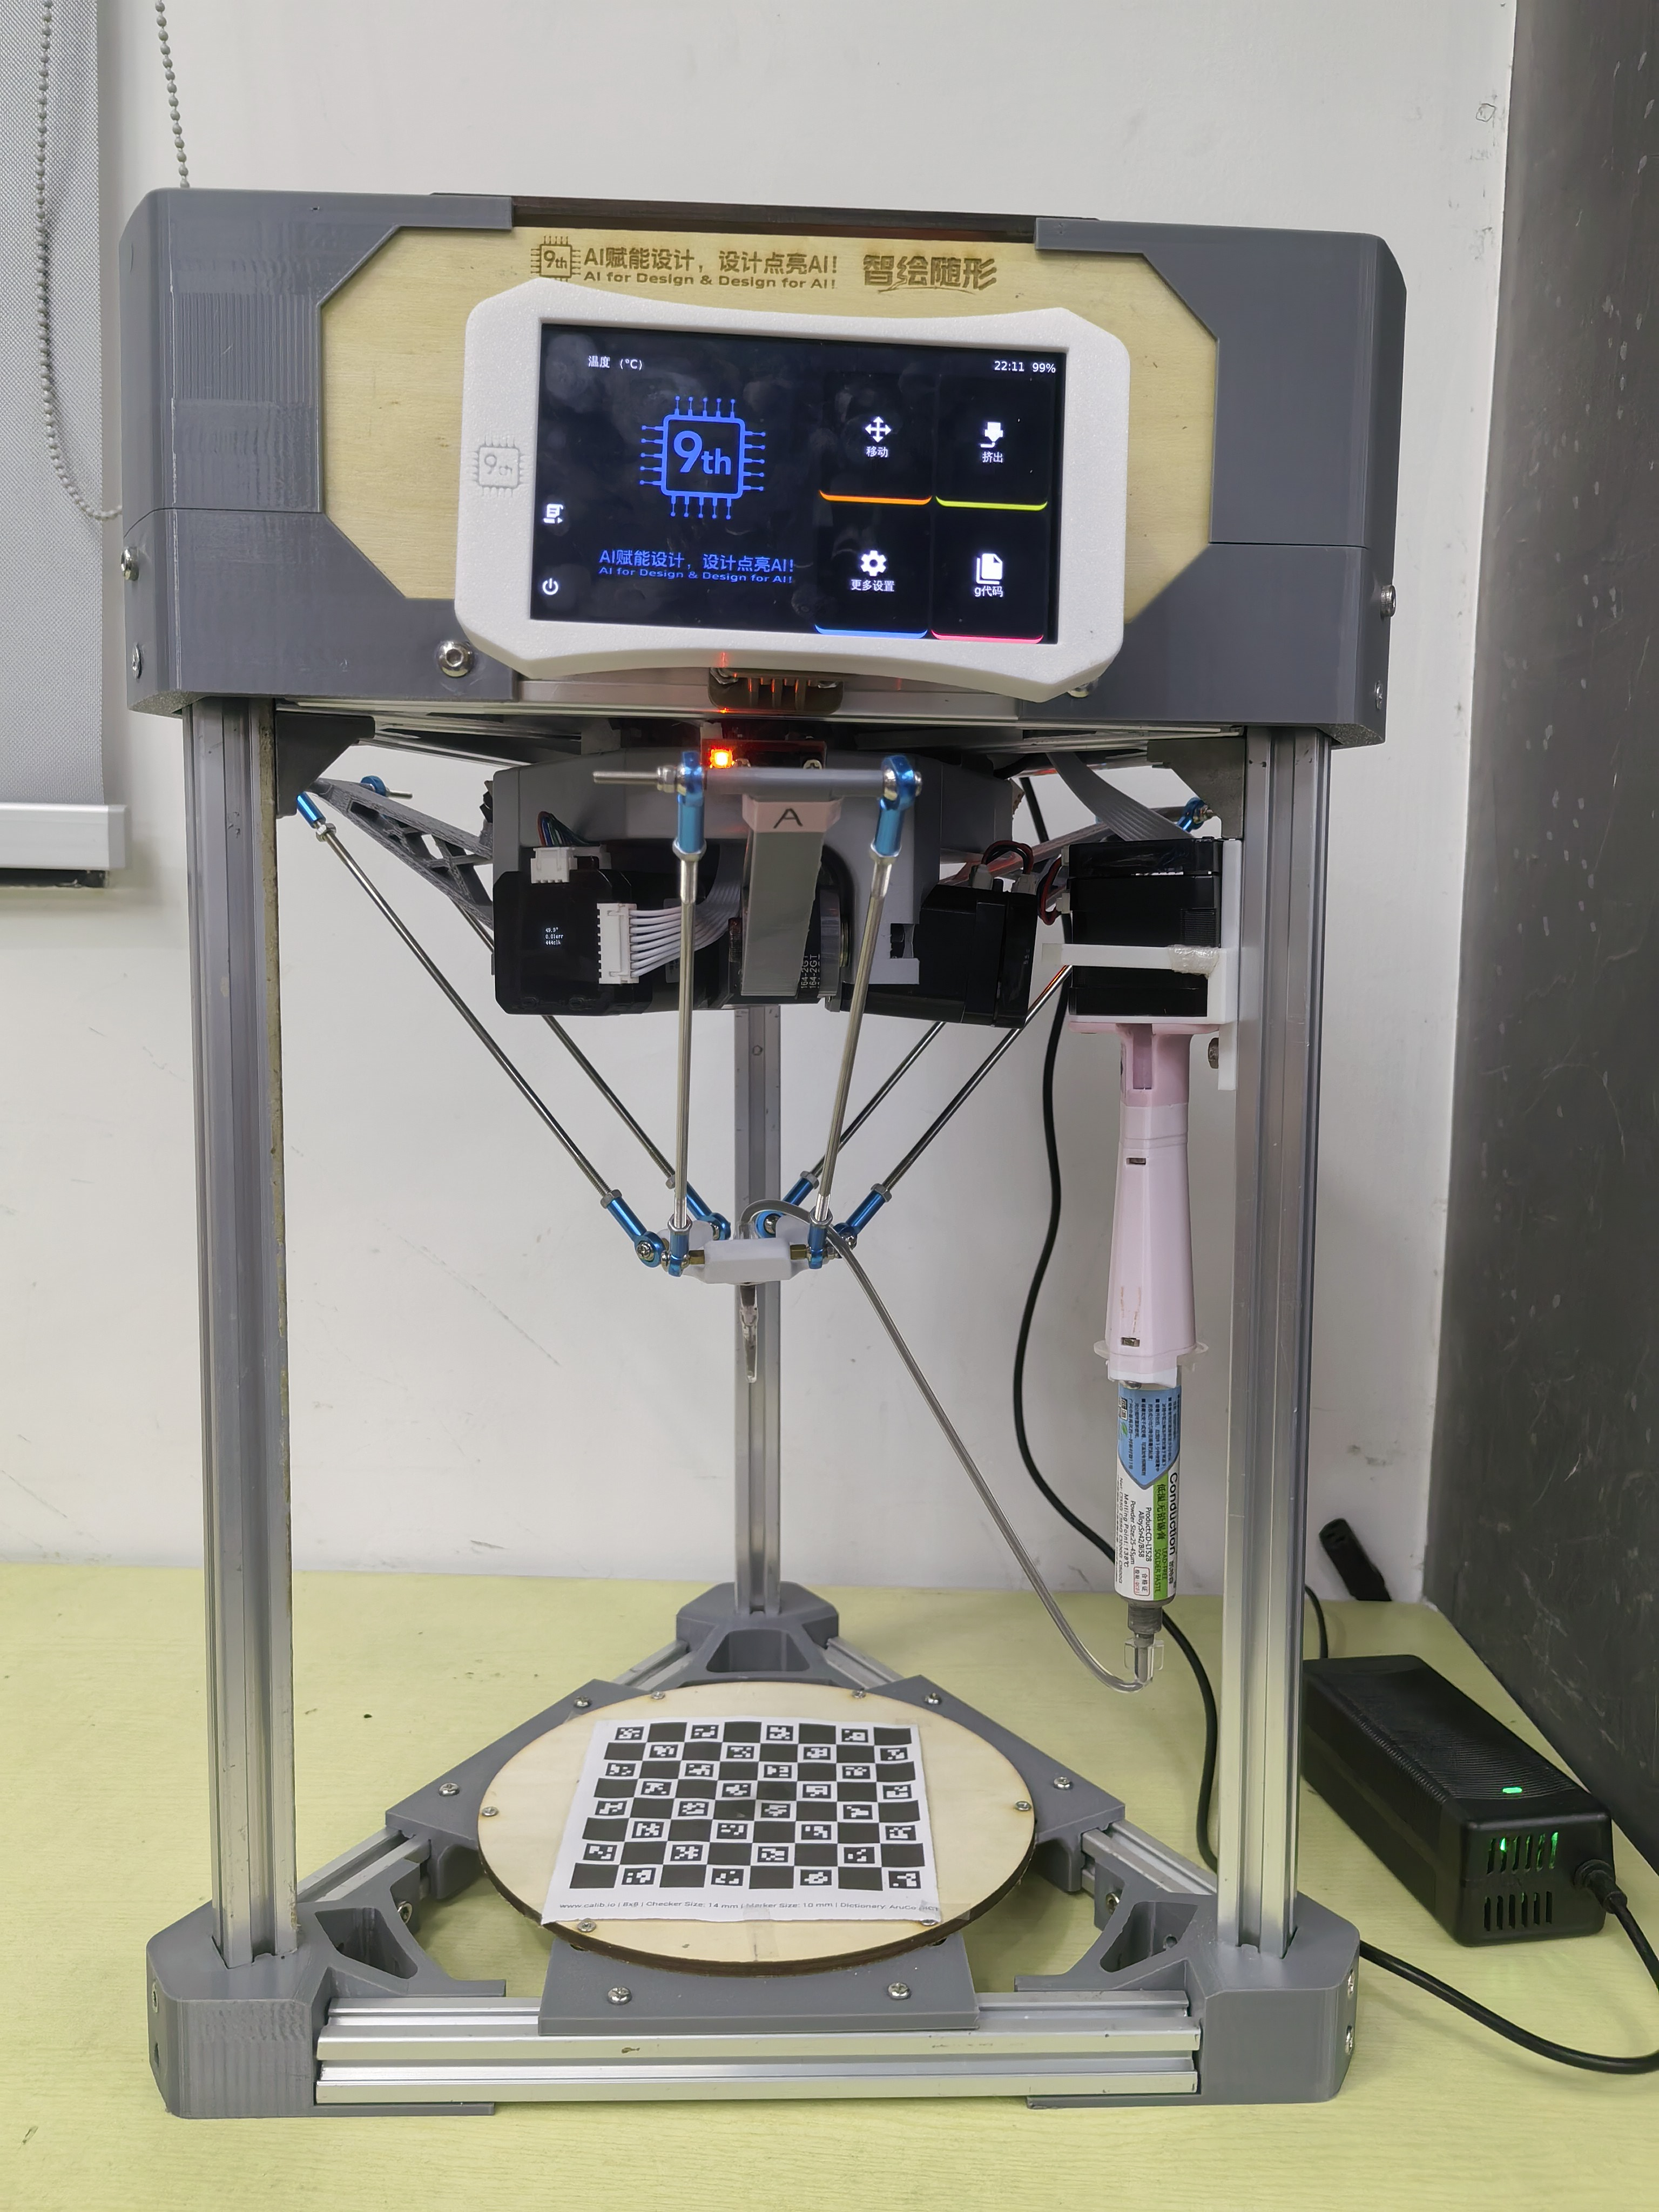
\includegraphics[width=\linewidth,keepaspectratio]{assets/img/正视图.jpg}
    \caption{系统正视图}
    \label{fig:system_front}
  \end{minipage}
  \hfill
  \begin{minipage}[t]{0.48\textwidth}
    \centering
    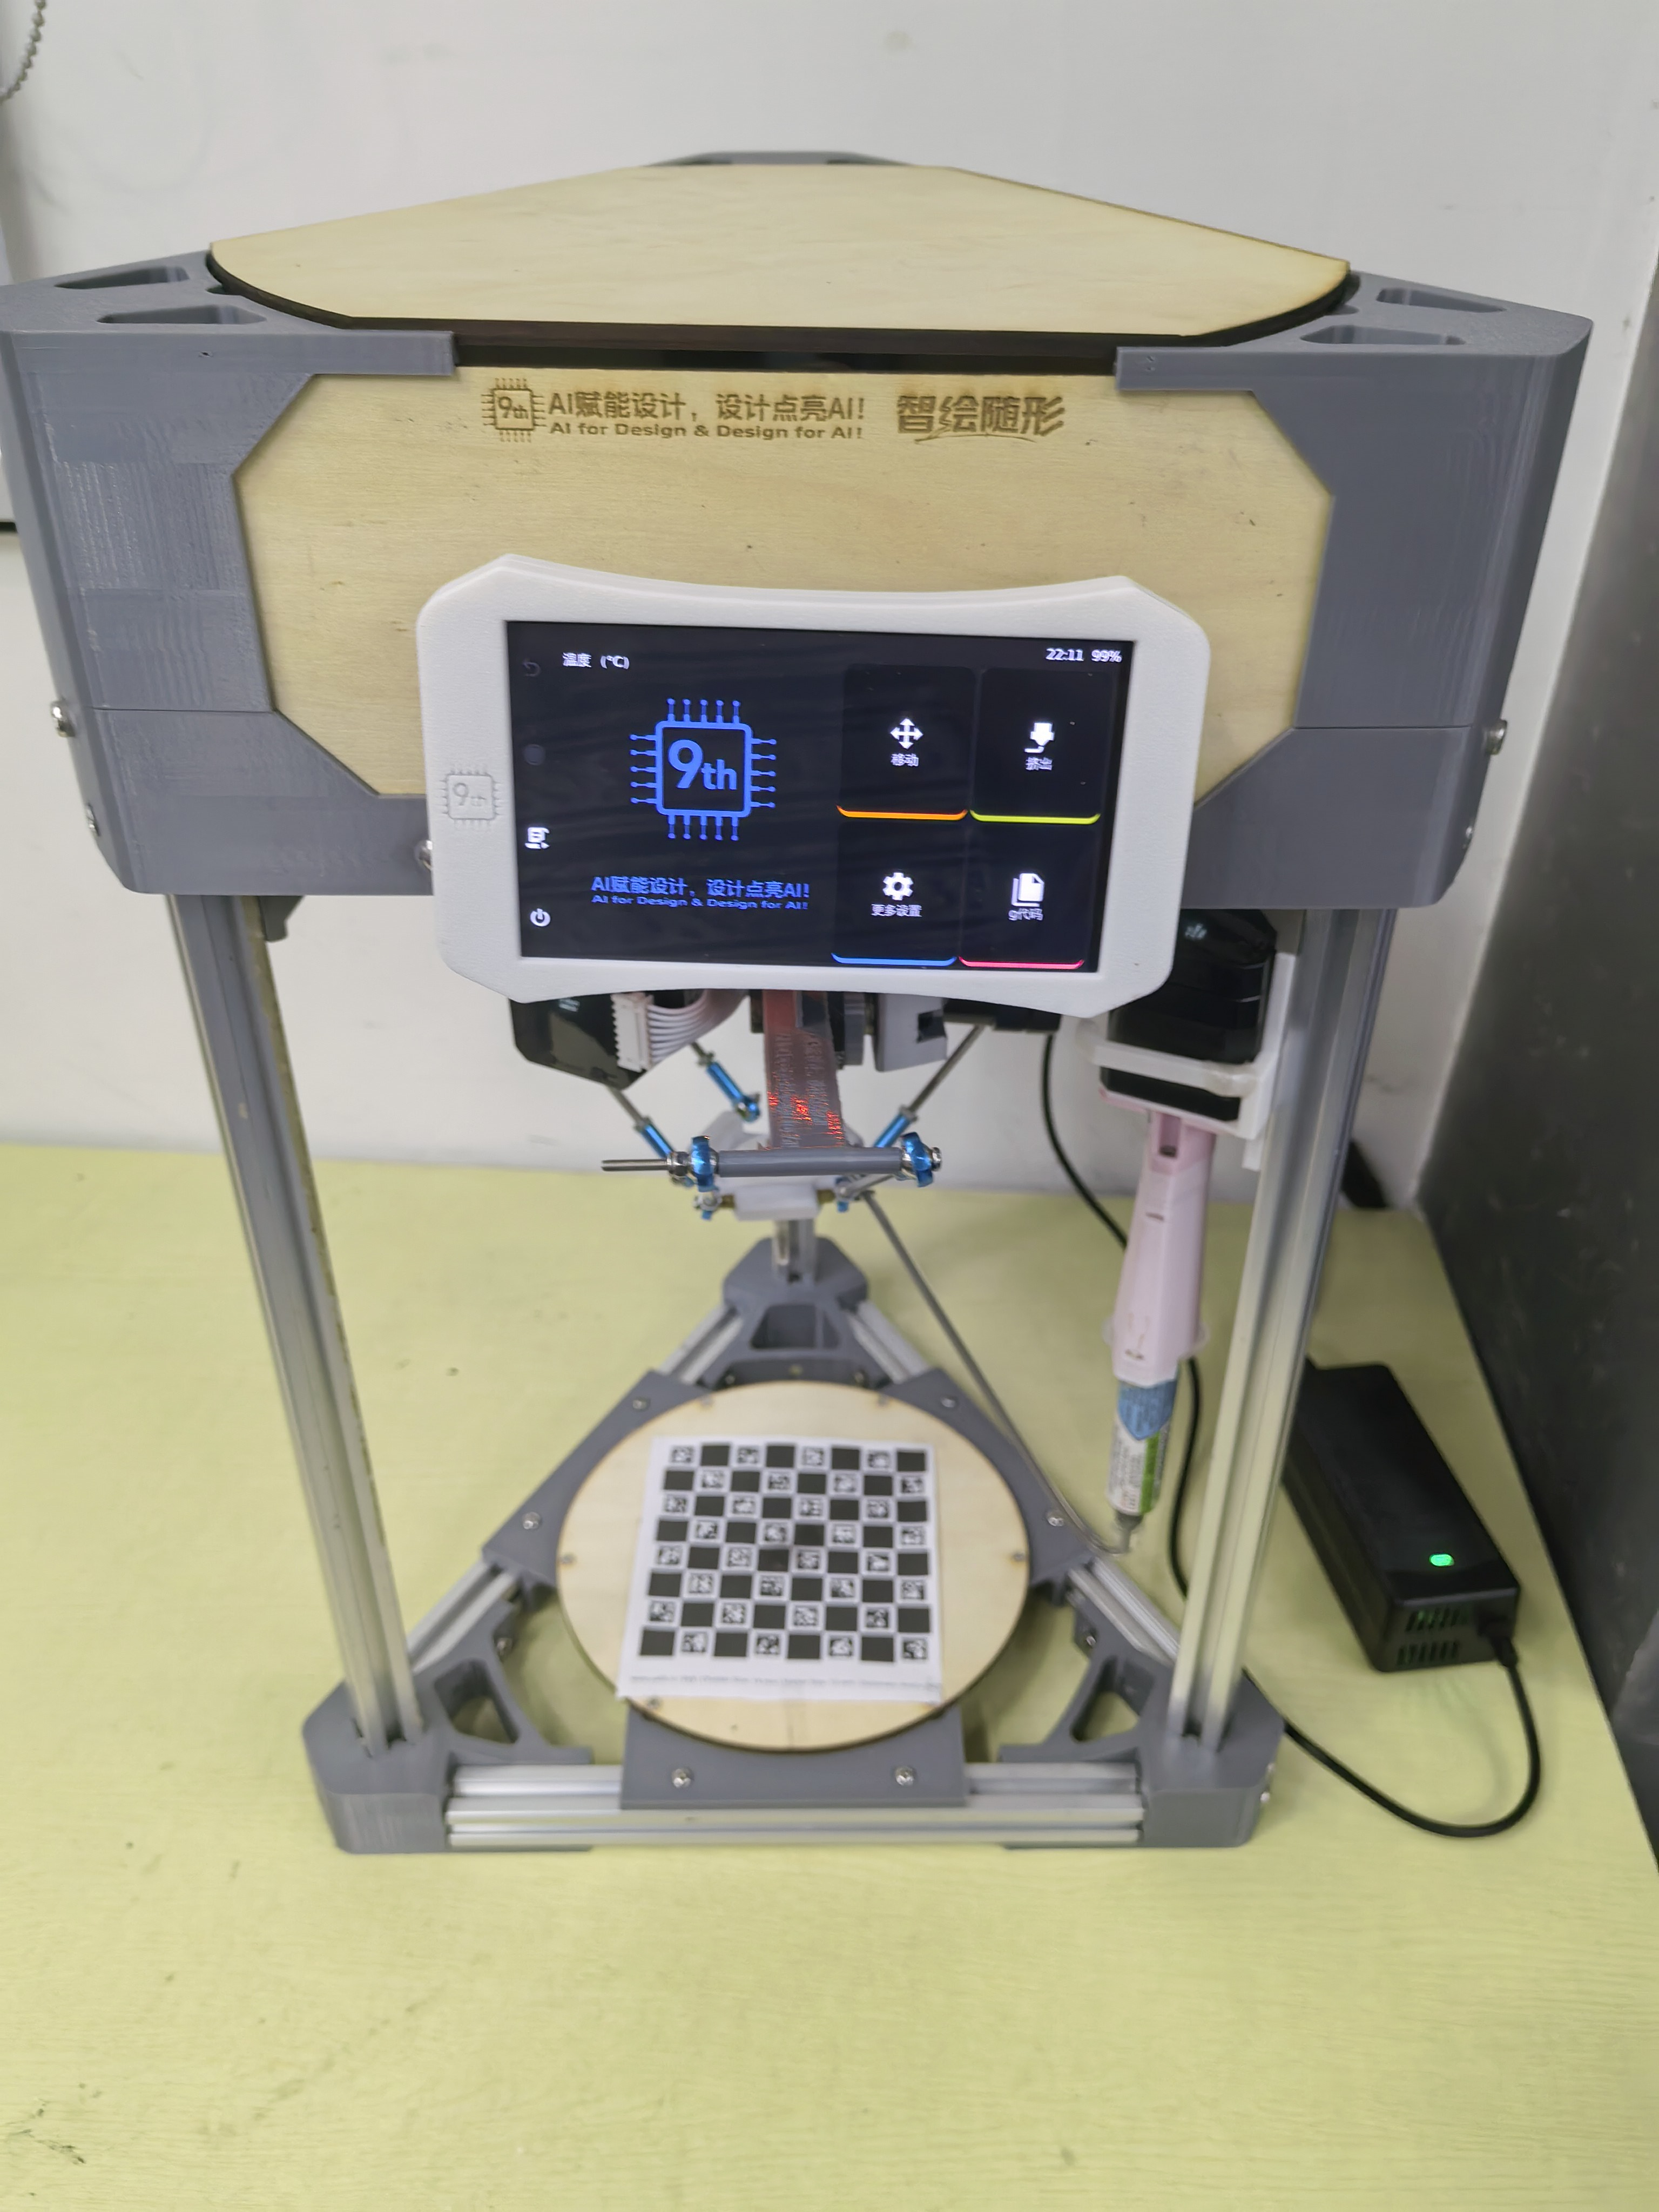
\includegraphics[width=\linewidth,keepaspectratio]{assets/img/45°视图.jpg}
    \caption{斜45°全局图}
    \label{fig:45}
  \end{minipage}
\end{figure}

\subsection{工程成果}
工程成果涵盖机械、电路和软件三个层面。机械部分完成 Delta 并联机构及其末端执行器的装配与调试（如图~\ref{fig:delta_mechanism}和图~\ref{fig:tools}）；电路部分完成 STM32F407 控制板及驱动模块的设计与制作（如图~\ref{fig:circuit} 和图~\ref{fig:PCB}）；软件部分完成桌面端上位机与本机触控屏的开发，相关模块界面已在第二部分详述。
\subsubsection{机械成果}
\begin{figure}[htbp]
  \centering
  \begin{minipage}[t]{0.48\textwidth}
    \centering
    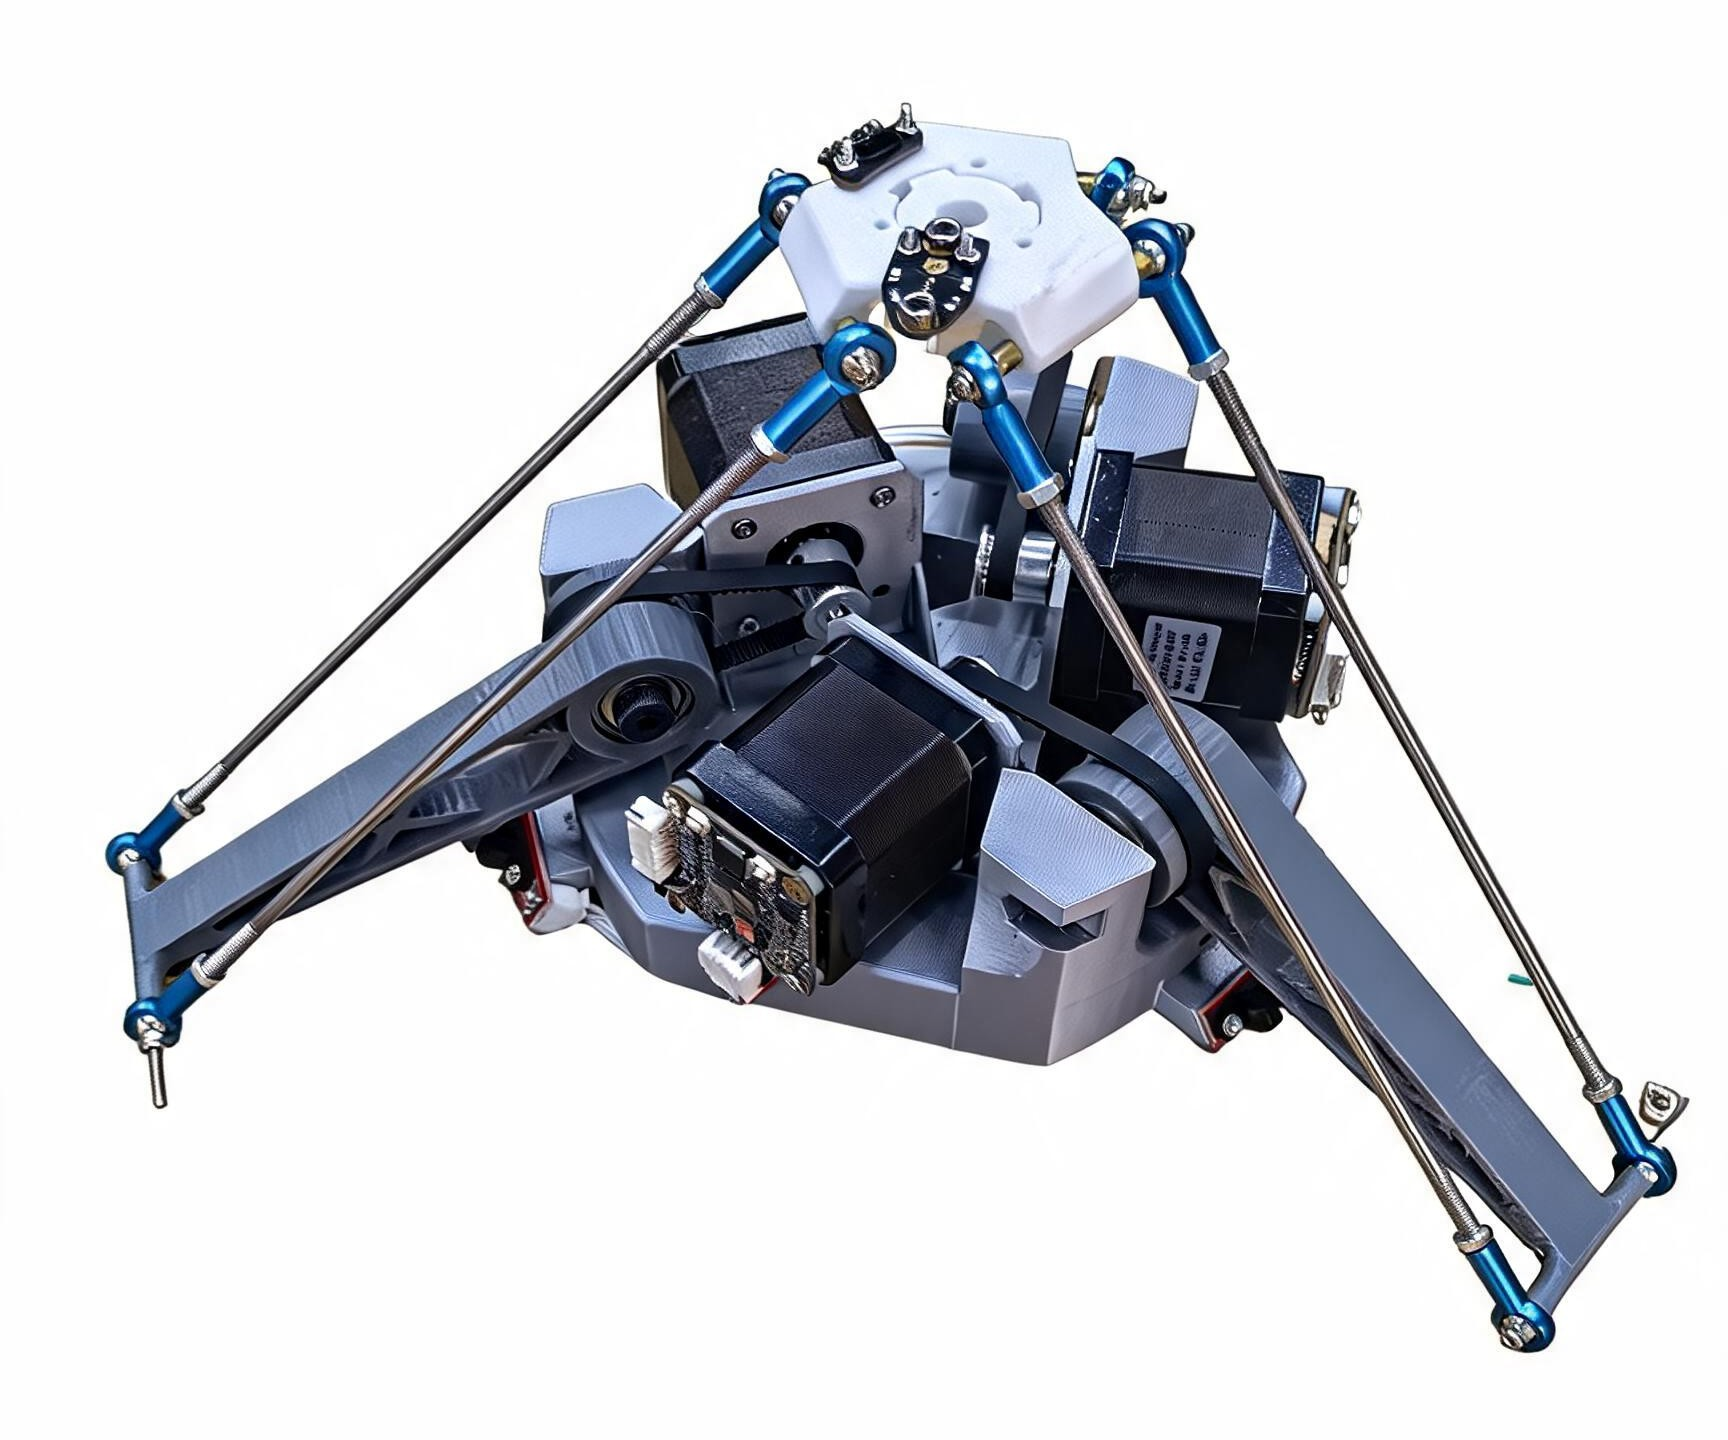
\includegraphics[width=\linewidth,keepaspectratio]{assets/img/机械结构.jpeg}
    \caption{Delta 并联机构实物图}
    \label{fig:delta_mechanism}
  \end{minipage}
  \hfill
  \begin{minipage}[t]{0.48\textwidth}
    \centering
    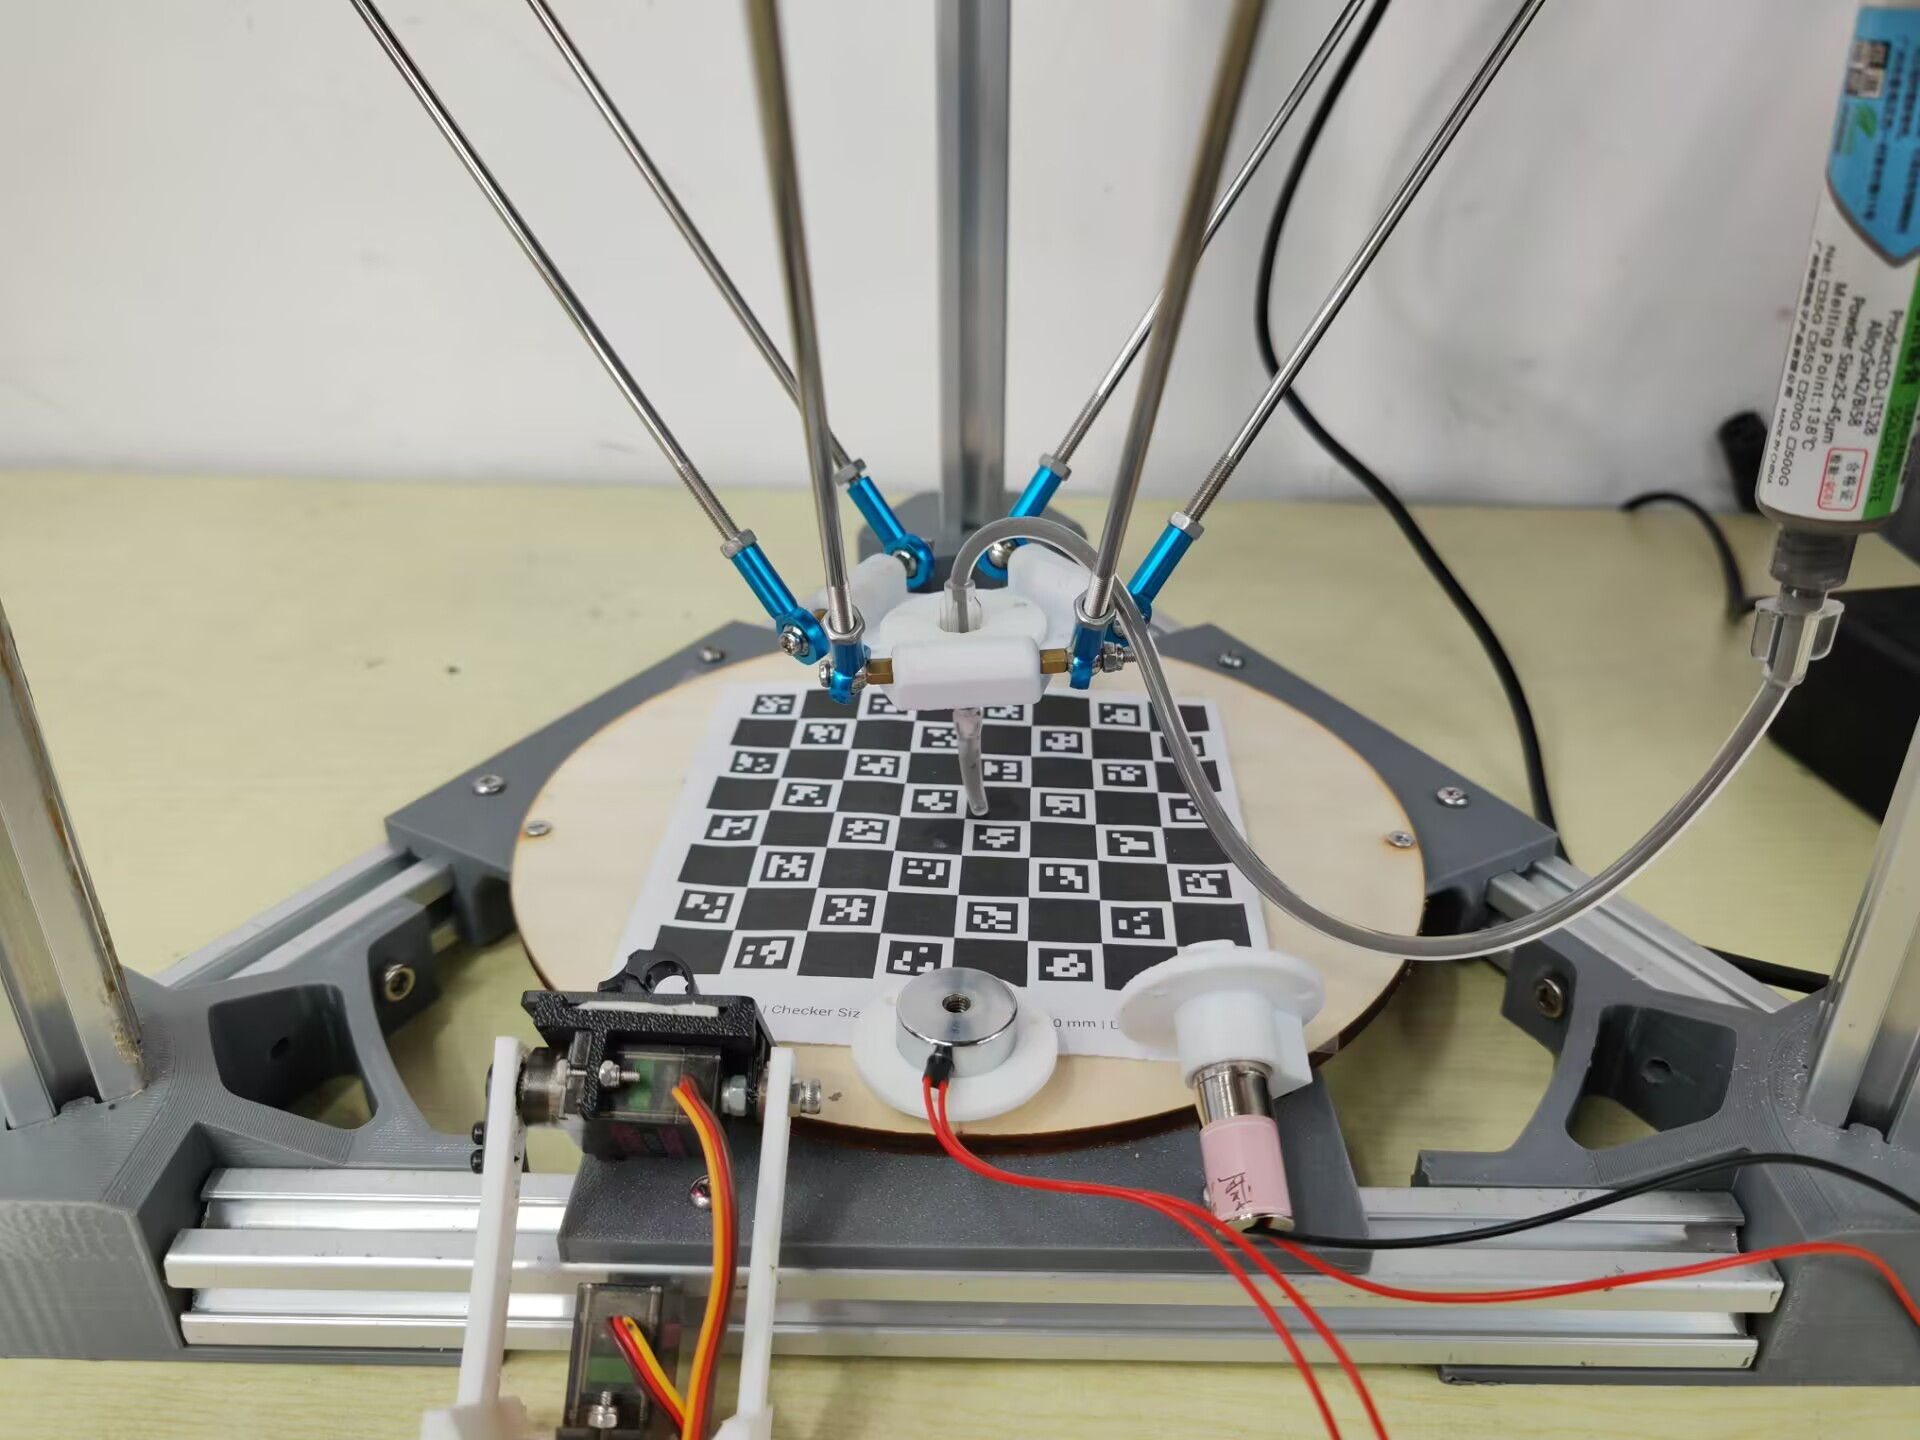
\includegraphics[width=\linewidth,keepaspectratio]{assets/img/工具头.jpg}
    \caption{多种工具头实物图}
    \label{fig:tools}
  \end{minipage}
\end{figure}

\subsubsection{电路成果}
\begin{figure}[htbp]
  \centering
  \begin{minipage}[t]{0.48\textwidth}
    \centering
    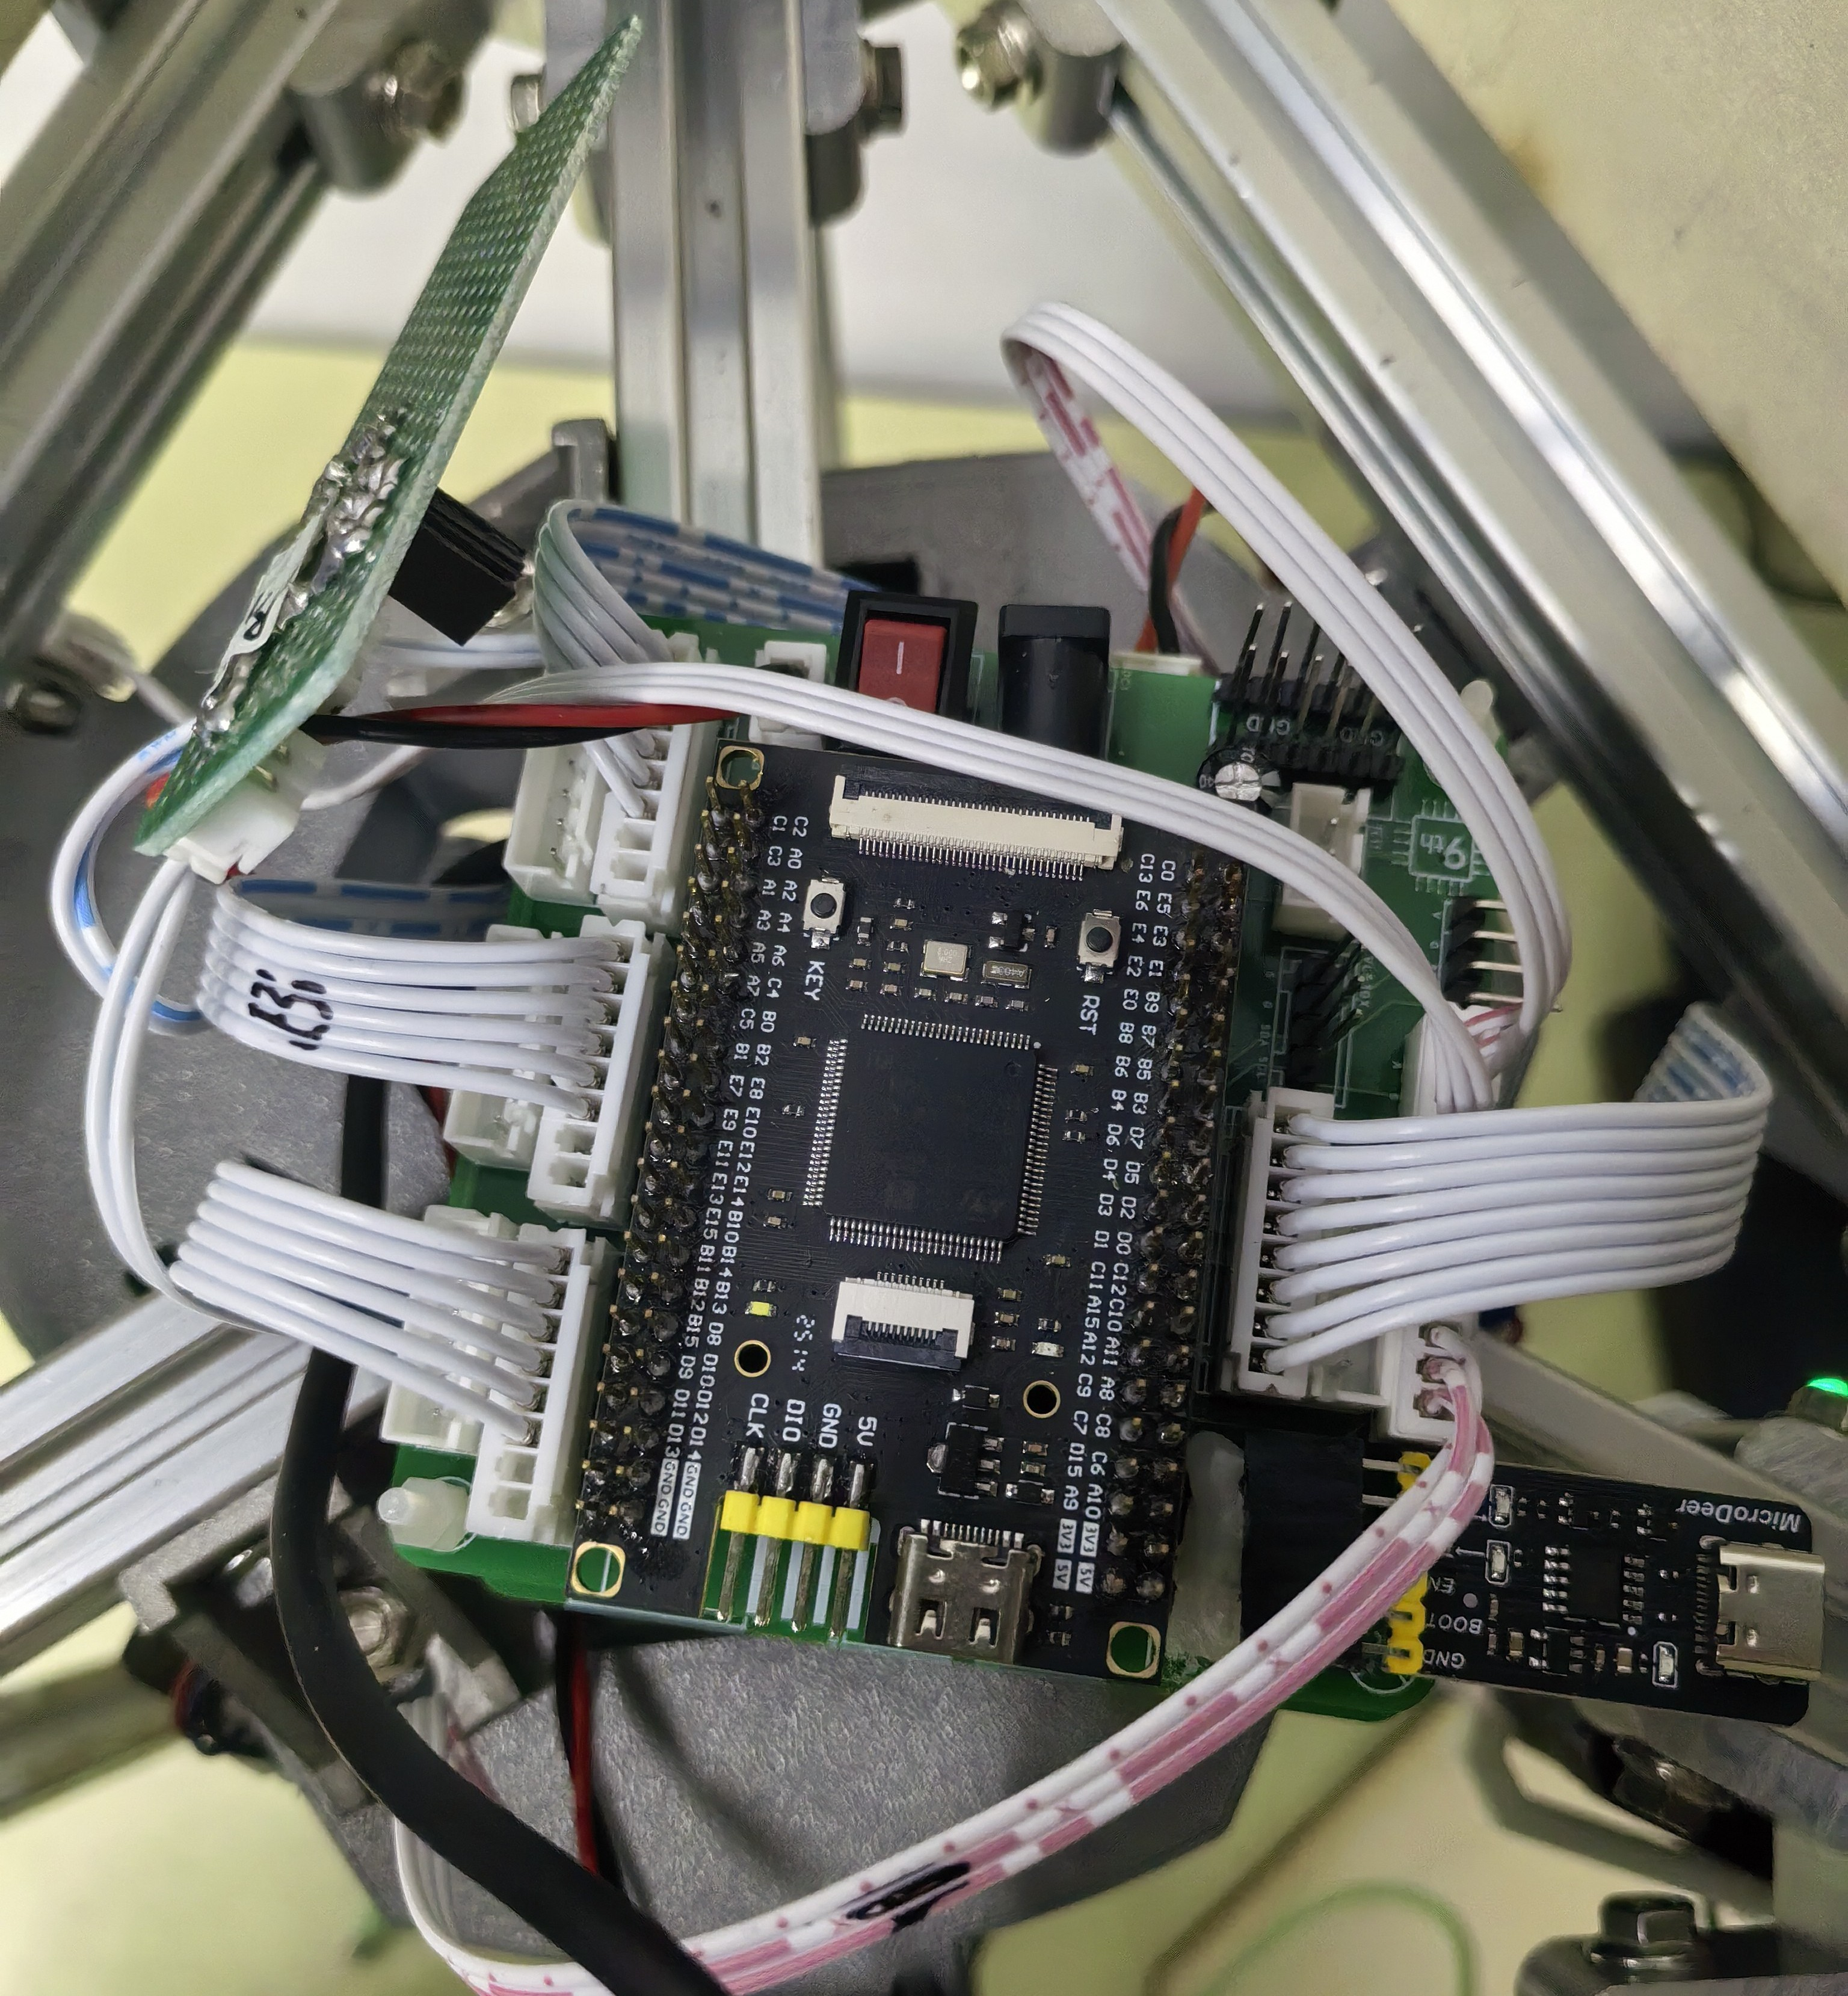
\includegraphics[width=\linewidth,keepaspectratio]{assets/img/电路板.jpg}
    \caption{电路板实物图}
    \label{fig:circuit}
  \end{minipage}
  \hfill
  \begin{minipage}[t]{0.48\textwidth}
    \centering
    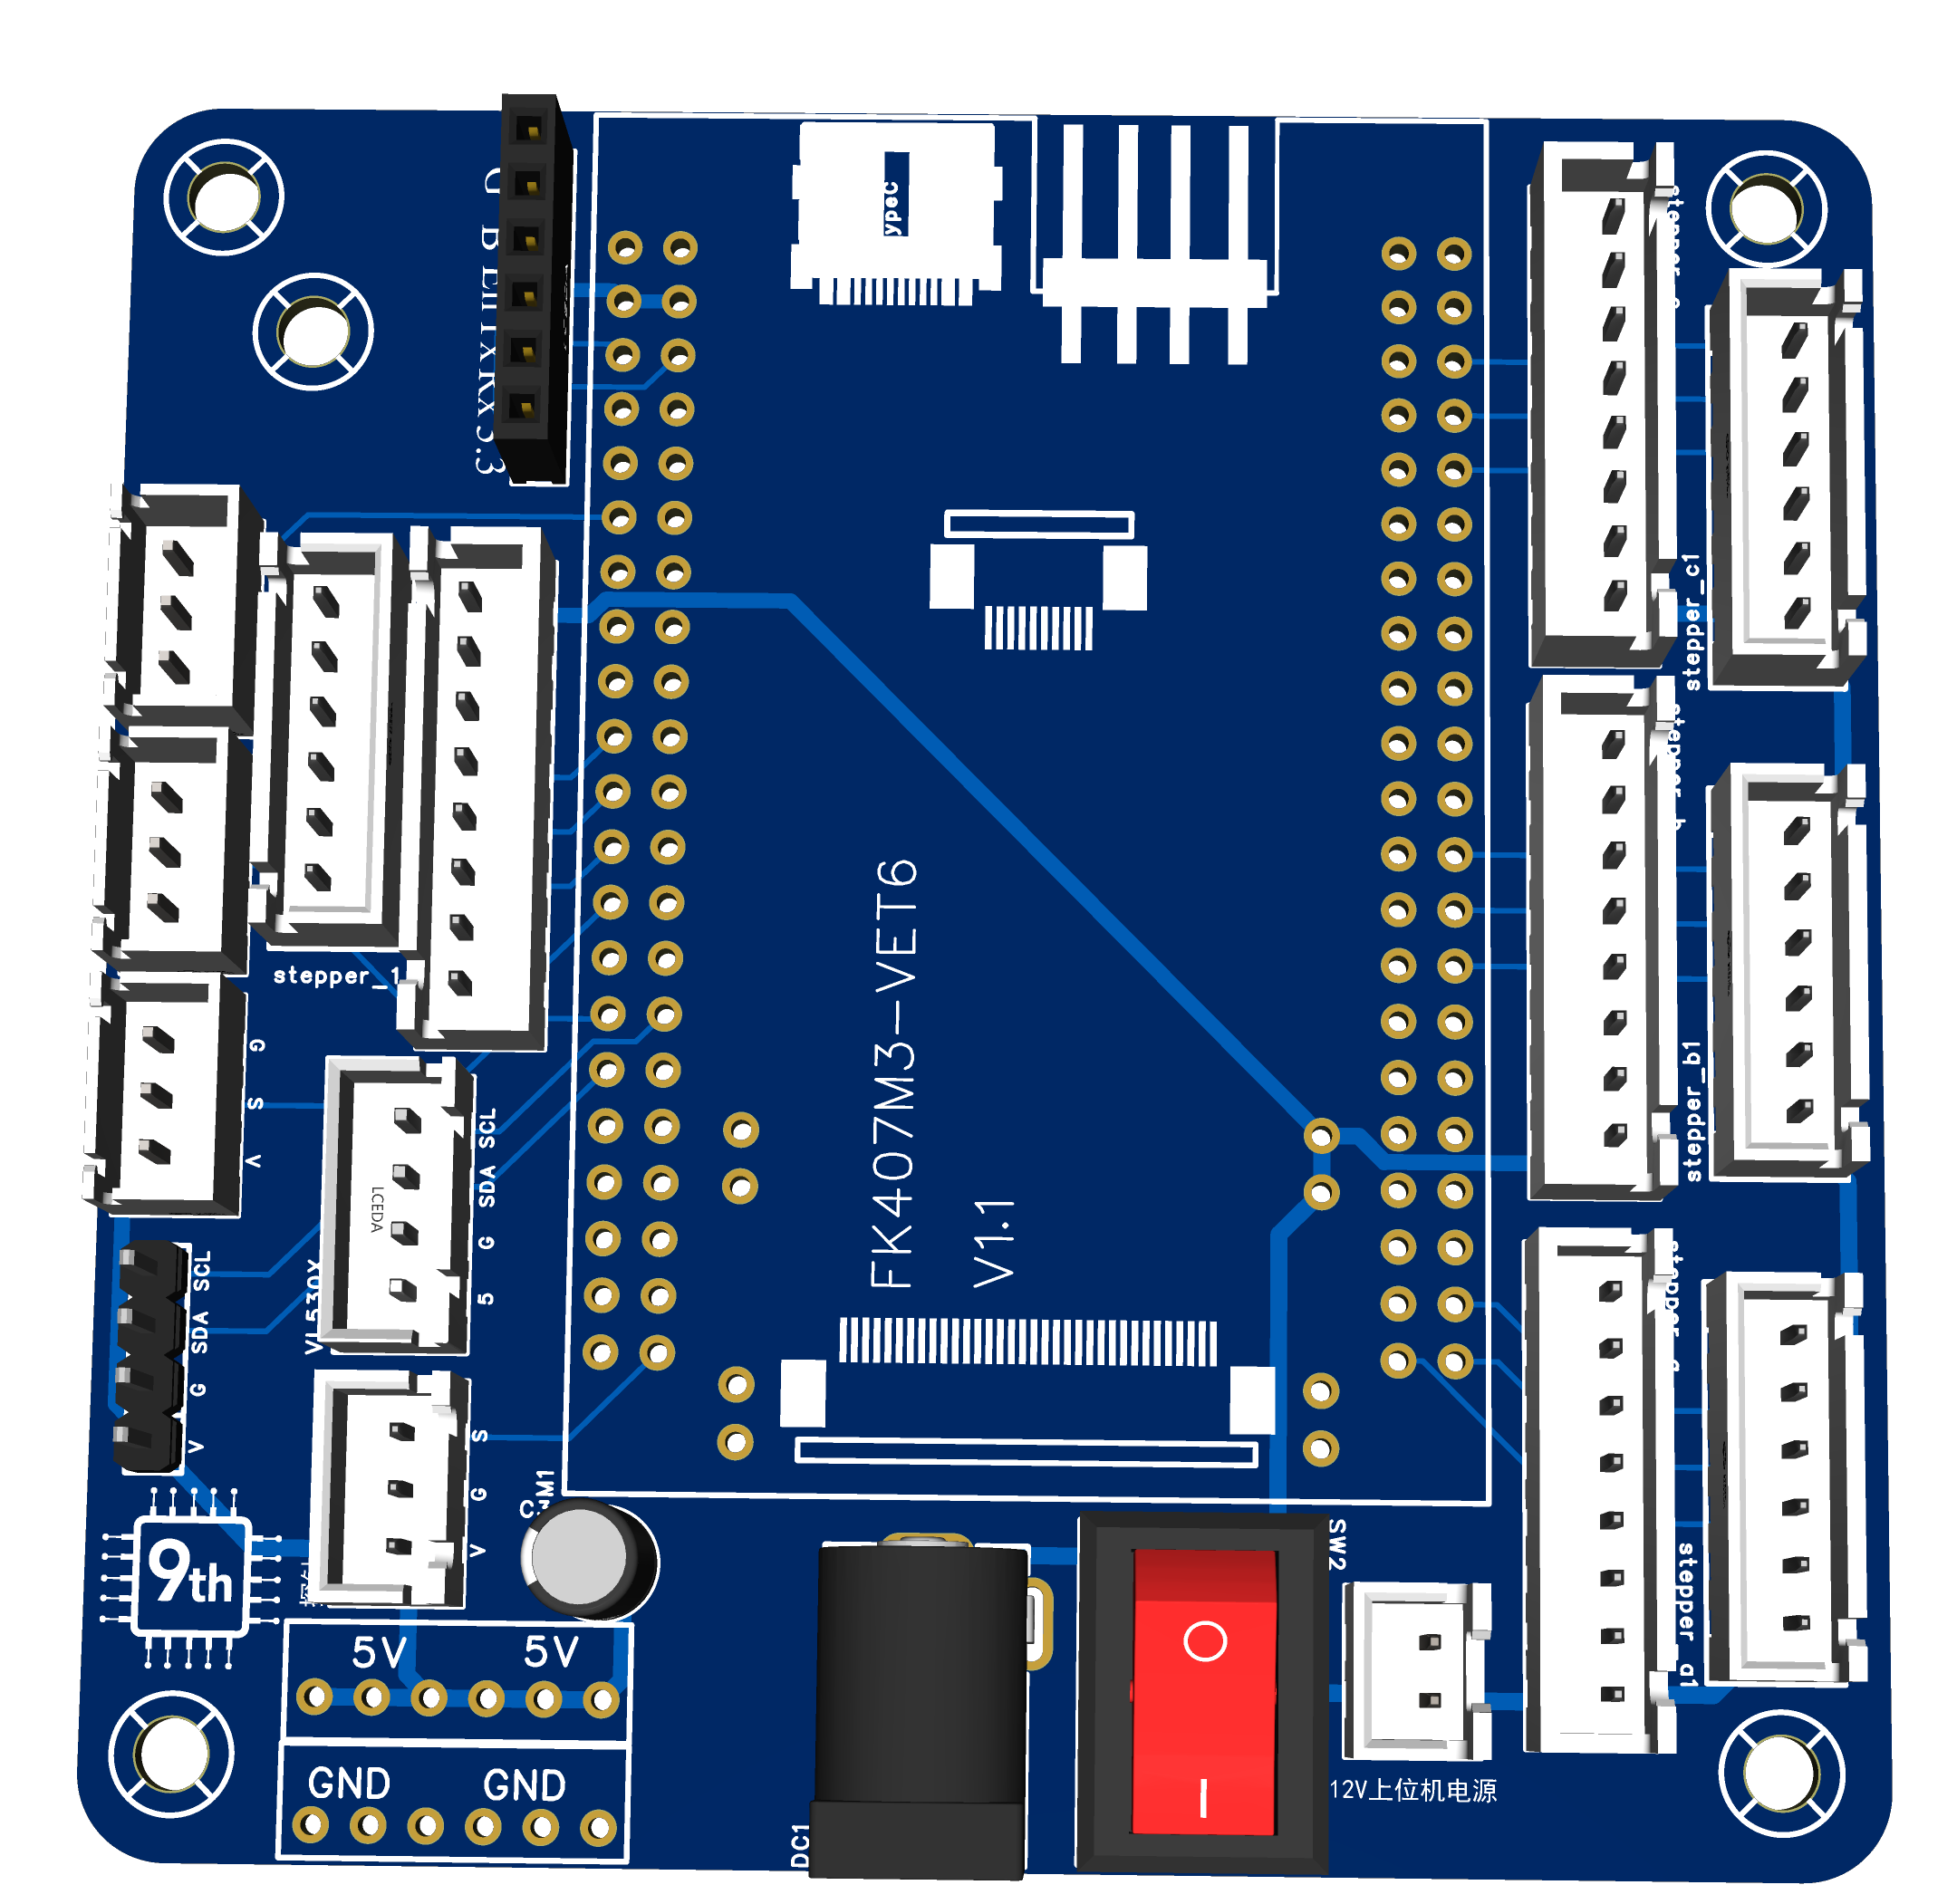
\includegraphics[width=\linewidth,keepaspectratio]{assets/img/PCB.png}
    \caption{PCB 3D 渲染图}
    \label{fig:PCB}
  \end{minipage}
\end{figure}

\subsubsection{软件成果}
桌面端软件界面如图~\ref{fig:control_panel}、图~\ref{fig:param_panel}、图~\ref{fig:curve_panel}、图~\ref{fig:photo_panel}、图~\ref{fig:calibration_panel} 和图~\ref{fig:trajectory_panel} 所示；本机触控屏界面如图~\ref{fig:main_panel} 和图~\ref{fig:running_panel} 所示。
桌面端软件图标如图\ref{fig:icon}所示：
\begin{figure}[htbp]
  \centering
  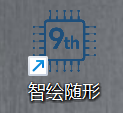
\includegraphics[width=0.4\textwidth,keepaspectratio]{assets/img/icon.png}
  \caption{桌面端软件图标}
  \label{fig:icon}
\end{figure}

\subsection{特性成果}

本作品围绕“曲面作业时末端轨迹能否准确落到目标坐标”进行了视觉标定与运动精度验证。测试时，上位机控制 Delta 机构依次运动到预设网格点，通过相机识别 ChArUco/AprilTag 标定板\cite{garrido2014aruco,olson2011apriltag}得到实际视觉坐标，再将视觉坐标转换到机械坐标系，与 G-code 指令目标位置进行比较。误差统计覆盖 $X=-40\sim40$\,mm、$Y=-20\sim25$\,mm、$Z=55/65/75$\,mm 的三层空间采样，共采集 150 组数据，其中 144 组有效。

从标定结果可见，相机内参平均重投影误差为 0.215\,px，说明角点/标志点检测具有较好的图像测量稳定性。在未进行坐标补偿时，末端 XY 平面 RMS 误差为 3.10\,mm，最大 XY 误差为 4.82\,mm；经过坐标拟合后，系统采用 XY 仿射补偿和 Z 向偏移修正，将补偿后验证 RMS XY 误差降至 0.41\,mm，最大 XY 误差降至 1.04\,mm，RMS XY 误差降低约 86.9\%。三层高度下的补偿后 RMS XY 误差分别为 0.486\,mm、0.348\,mm 和 0.364\,mm，说明补偿参数在测试高度范围内具有较好一致性。

为进一步验证补偿模型在非标定高度平面上的适用性，系统还在未参与 Stage 4 坐标拟合的 $Z=30/40$\,mm 平面进行了留出采样验证。该组测试沿用由 $Z=55/65/75$\,mm 标定数据生成的补偿参数，不重新拟合坐标变换；两层均覆盖同一 $X/Y$ 工作范围，每层 25 个网格点并重复 2 次，共得到 100 组有效样本。结果显示，非标定平面上的综合 RMS XY 误差为 0.93\,mm，最大 XY 误差为 1.88\,mm，其中 $Z=30$\,mm 层 RMS XY 误差为 1.009\,mm，$Z=40$\,mm 层为 0.835\,mm。与标定高度内的 0.41\,mm RMS XY 误差相比，非标定平面误差有所增大，但仍保持在约 1\,mm RMS、2\,mm 最大误差范围内，说明当前视觉补偿对标定高度外的平面仍具备可用的 XY 定位泛化能力。该组数据中的平均 Z 偏差约为 -1.84\,mm，提示后续若需要更高的高度方向精度，可进一步引入随 Z 高度变化的补偿模型。

\begin{table}[htbp]
  \centering
  \begin{tabular}{p{0.35\textwidth}p{0.48\textwidth}}
    \toprule
    量化项目 & 测试结果 \\
    \midrule
    相机内参平均重投影误差 & 0.215\,px \\
    有效运动误差样本 & 144 组，覆盖 $X=-40\sim40$\,mm、$Y=-20\sim25$\,mm、$Z=55/65/75$\,mm \\
    标定补偿前 XY 误差 & RMS = 3.10\,mm，最大 = 4.82\,mm \\
    标定补偿后 XY 误差 & RMS = 0.41\,mm，最大 = 1.04\,mm \\
    XY 精度提升幅度 & RMS 误差降低约 86.9\%，最大误差降低约 78.5\% \\
    分层 RMS XY 误差 & 55\,mm 层为 0.486\,mm，65\,mm 层为 0.348\,mm，75\,mm 层为 0.364\,mm \\
    Z 向偏差情况 & 平均 Z 偏差由 +0.879\,mm 修正为 -0.287\,mm，补偿后平均绝对误差约 1.10\,mm \\
    非标定 Z 平面验证 & $Z=30/40$\,mm，100 组有效样本；RMS XY = 0.93\,mm，最大 XY = 1.88\,mm \\
    非标定平面 RMS XY 误差 & 30\,mm 层为 1.009\,mm，40\,mm 层为 0.835\,mm \\
    非标定平面 Z 向偏差 & 平均 Z 偏差约 -1.84\,mm，Z 向平均绝对误差约 2.04\,mm \\
    \bottomrule
  \end{tabular}
  \caption{视觉标定与运动精度验证结果}
  \label{tab:visual-motion-accuracy}
\end{table}

图 \ref{fig:visual_calibration_evidence} 给出了视觉标定过程中的 ChArUco 检测叠加图和补偿后的误差网格。图中标定板角点和编号能够被稳定识别，误差网格中目标点与视觉测得点基本重合，说明视觉坐标到机械坐标的映射可用于实际轨迹校准。图 \ref{fig:visual_coordinate_fit_summary} 进一步展示了坐标拟合前后的残差变化，红色残差为初始误差，蓝色残差为拟合补偿后的误差；三层高度下残差向量明显缩短，与表 \ref{tab:visual-motion-accuracy} 中的误差下降结果一致。图 \ref{fig:visual_holdout_error_grid} 给出了 $Z=30/40$\,mm 非标定平面的留出验证结果，用于说明补偿模型在未参与标定高度上的实际定位表现。

\begin{figure}[htbp]
  \centering
  \begin{minipage}[t]{0.42\textwidth}
    \centering
    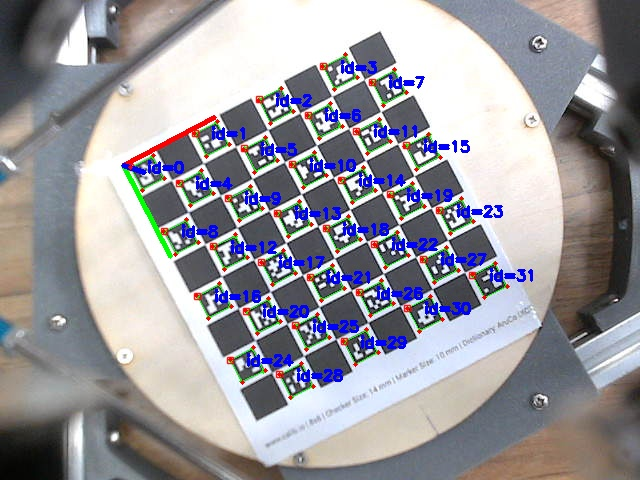
\includegraphics[width=\linewidth,keepaspectratio]{assets/img/visual_charuco_overlay.jpg}\\[0.2em]
    {\small （a）ChArUco 外参标定叠加图}
  \end{minipage}
  \hfill
  \begin{minipage}[t]{0.54\textwidth}
    \centering
    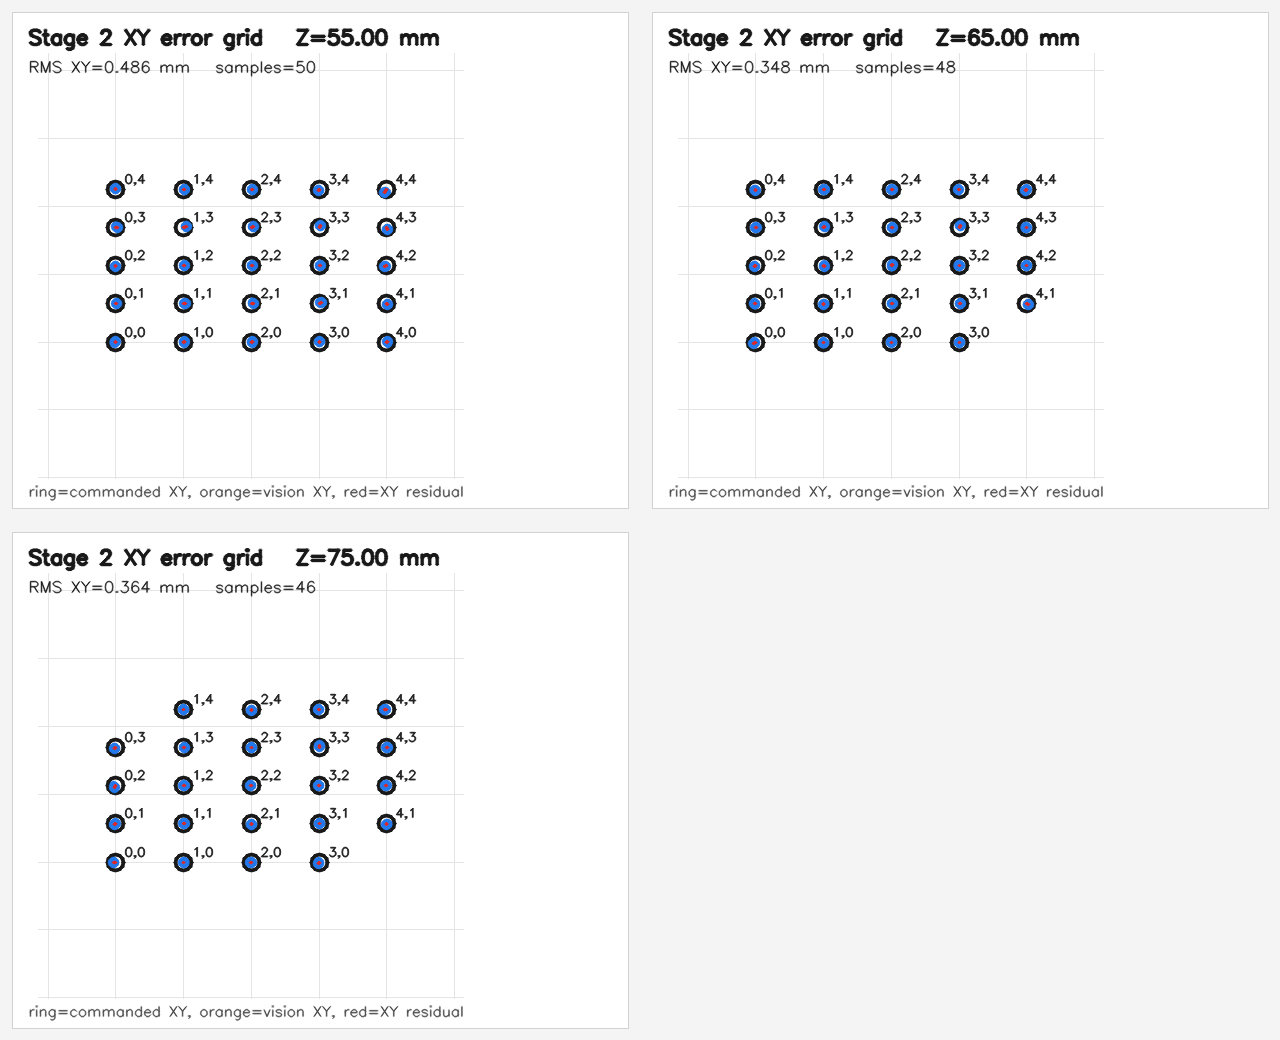
\includegraphics[width=\linewidth,keepaspectratio]{assets/img/visual_validation_error_grid.png}\\[0.2em]
    {\small （b）补偿后 XY 误差网格}
  \end{minipage}
  \caption{视觉标定结果与补偿后误差验证图}
  \label{fig:visual_calibration_evidence}
\end{figure}

\begin{figure}[htbp]
  \centering
  \begin{minipage}[t]{0.48\textwidth}
    \centering
    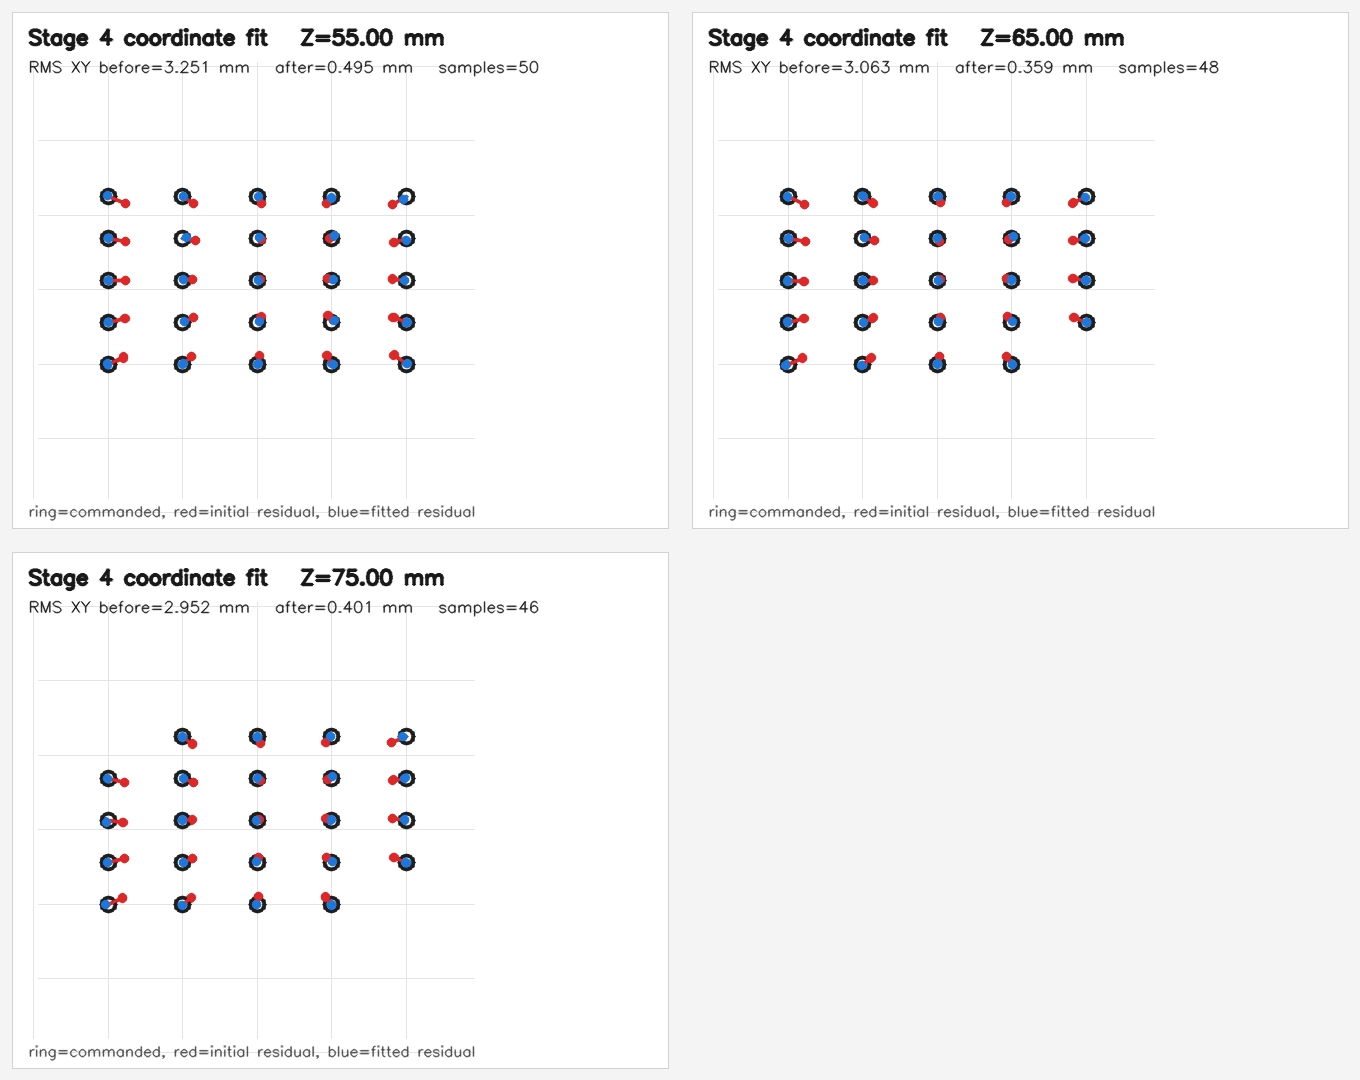
\includegraphics[width=\linewidth,keepaspectratio]{assets/img/visual_coordinate_fit_summary.png}
    \caption{坐标拟合前后残差对比}
    \label{fig:visual_coordinate_fit_summary}
  \end{minipage}
  \hfill
  \begin{minipage}[t]{0.48\textwidth}
    \centering
    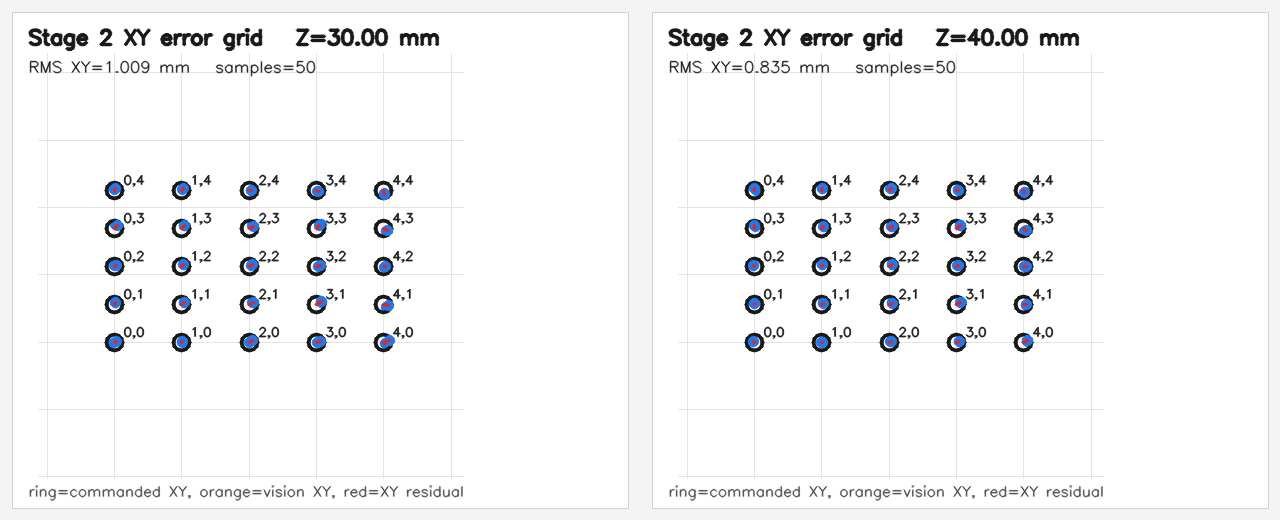
\includegraphics[width=\linewidth,keepaspectratio]{assets/img/visual_holdout_error_grid.png}
    \caption{非标定 Z 平面留出误差采样验证}
    \label{fig:visual_holdout_error_grid}
  \end{minipage}
\end{figure}

综合上述测试结果，系统已经形成“视觉采集--坐标标定--误差采样--补偿验证”的闭环调试流程。该流程使平台能够将毫米级初始装配误差压缩到亚毫米级 XY 定位误差范围内，为曲面恒距喷涂、导电材料喷印和精细路径复现提供了可量化的运动精度基础。

\partheading{第四部分}{总结}

\subsection{可扩展之处}
本作品目前已经完成曲面恒距轨迹生成、视觉标定补偿和多末端执行验证，后续仍可从末端、机构和算法三方面继续扩展。末端方面，可进一步优化喷头结构，增加流量闭环、雾化控制或多材料切换能力，使其适应导电油墨、涂料、胶体等不同介质。机构方面，可在 Delta 动平台末端增加两自由度舵机云台，使喷头法向能够随曲面姿态调整，从“恒距”进一步扩展到“恒距恒角度”作业。算法方面，可引入随 Z 高度变化的补偿模型，并结合在线视觉反馈进行二次修正，以提升复杂曲面和更大工作范围下的稳定性。

\subsection{心得体会}
本项目的研发过程让我们体会到，机器人系统的难点并不只在某一个模块，而在机械、电子、控制和软件之间的整体配合。Delta 机构响应快、末端轻，但装配误差、连杆长度误差和手动测量误差会直接反映到末端轨迹上。早期调试时，我们主要依靠尺量和单点校准，虽然能够让机构运动起来，但在曲面路径复现时仍会出现毫米级偏差，说明仅靠理论运动学模型\cite{hadfield2020delta}难以满足实际作业需求。

在感知方案上，我们最初尝试使用 VL53L0X 激光测距传感器获取高度信息，但受量程、反射率和安装角度影响，数据稳定性不足，难以支撑精细喷印。后续改为单目视觉标定与坐标补偿方案，通过 ChArUco/AprilTag 标定板采集实际位置，再建立视觉坐标与机械坐标之间的补偿关系\cite{zhang2000calibration,garrido2014aruco,olson2011apriltag}，XY 定位误差明显下降。这个过程也让我们认识到，精度提升往往不是单纯更换一个器件，而是建立“测量--分析--补偿--验证”的闭环。

通过本次设计，我们完成了从机构搭建、驱动调试、上位机开发到轨迹验证的完整流程，也积累了曲面作业平台的工程经验。后续如果继续完善喷头、姿态自由度和在线反馈机制，该平台有望进一步用于曲面喷涂、柔性电子制造和教学科研验证等场景。

\partheading{第五部分}{参考文献}

\begin{thebibliography}{99}
\bibitem{clavel1988delta}
Clavel R. DELTA, a fast robot with parallel geometry[C]//Proceedings of the 18th International Symposium on Industrial Robots. 1988.

\bibitem{hadfield2020delta}
Hadfield H, Wei Y, Lasenby J. The forward and inverse kinematics of a Delta robot[R]. University of Cambridge Repository, 2020. \url{https://www.repository.cam.ac.uk/items/b080ea69-d294-4f7b-99c2-39cc64415f57}.

\bibitem{zhang2000calibration}
Zhang Z. A flexible new technique for camera calibration[J]. IEEE Transactions on Pattern Analysis and Machine Intelligence, 2000, 22(11): 1330--1334. DOI: \url{https://doi.org/10.1109/34.888718}.

\bibitem{garrido2014aruco}
Garrido-Jurado S, Munoz-Salinas R, Madrid-Cuevas F J, Medina-Carnicer R. Automatic generation and detection of highly reliable fiducial markers under occlusion[J]. Pattern Recognition, 2014, 47(6): 2280--2292. DOI: \url{https://doi.org/10.1016/j.patcog.2014.01.005}.

\bibitem{olson2011apriltag}
Olson E. AprilTag: A robust and flexible visual fiducial system[C]//2011 IEEE International Conference on Robotics and Automation. 2011: 3400--3407. DOI: \url{https://doi.org/10.1109/ICRA.2011.5979561}.

\bibitem{atkar2005coverage}
Atkar P N, Greenfield A, Conner D C, Choset H, Rizzi A A. Uniform coverage of automotive surface patches[J]. The International Journal of Robotics Research, 2005, 24(11): 883--898. DOI: \url{https://doi.org/10.1177/0278364905059067}.

\bibitem{lewis2006diw}
Lewis J A. Direct ink writing of 3D functional materials[J]. Advanced Functional Materials, 2006, 16(17): 2193--2204. DOI: \url{https://doi.org/10.1002/adfm.200600434}.

\bibitem{muth2014embedded}
Muth J T, Vogt D M, Truby R L, et al. Embedded 3D printing of strain sensors within highly stretchable elastomers[J]. Advanced Materials, 2014, 26(36): 6307--6312. DOI: \url{https://doi.org/10.1002/adma.201400334}.

\bibitem{valentine2017soft}
Valentine A D, Busbee T A, Boley J W, et al. Hybrid 3D printing of soft electronics[J]. Advanced Materials, 2017, 29(40): 1703817. DOI: \url{https://doi.org/10.1002/adma.201703817}.
\end{thebibliography}

\end{document}
